% Options for packages loaded elsewhere
\PassOptionsToPackage{unicode}{hyperref}
\PassOptionsToPackage{hyphens}{url}
%
\documentclass[
]{book}
\usepackage{lmodern}
\usepackage{amssymb,amsmath}
\usepackage{ifxetex,ifluatex}
\ifnum 0\ifxetex 1\fi\ifluatex 1\fi=0 % if pdftex
  \usepackage[T1]{fontenc}
  \usepackage[utf8]{inputenc}
  \usepackage{textcomp} % provide euro and other symbols
\else % if luatex or xetex
  \usepackage{unicode-math}
  \defaultfontfeatures{Scale=MatchLowercase}
  \defaultfontfeatures[\rmfamily]{Ligatures=TeX,Scale=1}
\fi
% Use upquote if available, for straight quotes in verbatim environments
\IfFileExists{upquote.sty}{\usepackage{upquote}}{}
\IfFileExists{microtype.sty}{% use microtype if available
  \usepackage[]{microtype}
  \UseMicrotypeSet[protrusion]{basicmath} % disable protrusion for tt fonts
}{}
\makeatletter
\@ifundefined{KOMAClassName}{% if non-KOMA class
  \IfFileExists{parskip.sty}{%
    \usepackage{parskip}
  }{% else
    \setlength{\parindent}{0pt}
    \setlength{\parskip}{6pt plus 2pt minus 1pt}}
}{% if KOMA class
  \KOMAoptions{parskip=half}}
\makeatother
\usepackage{xcolor}
\IfFileExists{xurl.sty}{\usepackage{xurl}}{} % add URL line breaks if available
\IfFileExists{bookmark.sty}{\usepackage{bookmark}}{\usepackage{hyperref}}
\hypersetup{
  pdftitle={Supplementary Materials: Code \& Results},
  pdfauthor={Trémolière B \& Gosling CJ},
  hidelinks,
  pdfcreator={LaTeX via pandoc}}
\urlstyle{same} % disable monospaced font for URLs
\usepackage{color}
\usepackage{fancyvrb}
\newcommand{\VerbBar}{|}
\newcommand{\VERB}{\Verb[commandchars=\\\{\}]}
\DefineVerbatimEnvironment{Highlighting}{Verbatim}{commandchars=\\\{\}}
% Add ',fontsize=\small' for more characters per line
\usepackage{framed}
\definecolor{shadecolor}{RGB}{248,248,248}
\newenvironment{Shaded}{\begin{snugshade}}{\end{snugshade}}
\newcommand{\AlertTok}[1]{\textcolor[rgb]{0.94,0.16,0.16}{#1}}
\newcommand{\AnnotationTok}[1]{\textcolor[rgb]{0.56,0.35,0.01}{\textbf{\textit{#1}}}}
\newcommand{\AttributeTok}[1]{\textcolor[rgb]{0.77,0.63,0.00}{#1}}
\newcommand{\BaseNTok}[1]{\textcolor[rgb]{0.00,0.00,0.81}{#1}}
\newcommand{\BuiltInTok}[1]{#1}
\newcommand{\CharTok}[1]{\textcolor[rgb]{0.31,0.60,0.02}{#1}}
\newcommand{\CommentTok}[1]{\textcolor[rgb]{0.56,0.35,0.01}{\textit{#1}}}
\newcommand{\CommentVarTok}[1]{\textcolor[rgb]{0.56,0.35,0.01}{\textbf{\textit{#1}}}}
\newcommand{\ConstantTok}[1]{\textcolor[rgb]{0.00,0.00,0.00}{#1}}
\newcommand{\ControlFlowTok}[1]{\textcolor[rgb]{0.13,0.29,0.53}{\textbf{#1}}}
\newcommand{\DataTypeTok}[1]{\textcolor[rgb]{0.13,0.29,0.53}{#1}}
\newcommand{\DecValTok}[1]{\textcolor[rgb]{0.00,0.00,0.81}{#1}}
\newcommand{\DocumentationTok}[1]{\textcolor[rgb]{0.56,0.35,0.01}{\textbf{\textit{#1}}}}
\newcommand{\ErrorTok}[1]{\textcolor[rgb]{0.64,0.00,0.00}{\textbf{#1}}}
\newcommand{\ExtensionTok}[1]{#1}
\newcommand{\FloatTok}[1]{\textcolor[rgb]{0.00,0.00,0.81}{#1}}
\newcommand{\FunctionTok}[1]{\textcolor[rgb]{0.00,0.00,0.00}{#1}}
\newcommand{\ImportTok}[1]{#1}
\newcommand{\InformationTok}[1]{\textcolor[rgb]{0.56,0.35,0.01}{\textbf{\textit{#1}}}}
\newcommand{\KeywordTok}[1]{\textcolor[rgb]{0.13,0.29,0.53}{\textbf{#1}}}
\newcommand{\NormalTok}[1]{#1}
\newcommand{\OperatorTok}[1]{\textcolor[rgb]{0.81,0.36,0.00}{\textbf{#1}}}
\newcommand{\OtherTok}[1]{\textcolor[rgb]{0.56,0.35,0.01}{#1}}
\newcommand{\PreprocessorTok}[1]{\textcolor[rgb]{0.56,0.35,0.01}{\textit{#1}}}
\newcommand{\RegionMarkerTok}[1]{#1}
\newcommand{\SpecialCharTok}[1]{\textcolor[rgb]{0.00,0.00,0.00}{#1}}
\newcommand{\SpecialStringTok}[1]{\textcolor[rgb]{0.31,0.60,0.02}{#1}}
\newcommand{\StringTok}[1]{\textcolor[rgb]{0.31,0.60,0.02}{#1}}
\newcommand{\VariableTok}[1]{\textcolor[rgb]{0.00,0.00,0.00}{#1}}
\newcommand{\VerbatimStringTok}[1]{\textcolor[rgb]{0.31,0.60,0.02}{#1}}
\newcommand{\WarningTok}[1]{\textcolor[rgb]{0.56,0.35,0.01}{\textbf{\textit{#1}}}}
\usepackage{longtable,booktabs}
% Correct order of tables after \paragraph or \subparagraph
\usepackage{etoolbox}
\makeatletter
\patchcmd\longtable{\par}{\if@noskipsec\mbox{}\fi\par}{}{}
\makeatother
% Allow footnotes in longtable head/foot
\IfFileExists{footnotehyper.sty}{\usepackage{footnotehyper}}{\usepackage{footnote}}
\makesavenoteenv{longtable}
\usepackage{graphicx,grffile}
\makeatletter
\def\maxwidth{\ifdim\Gin@nat@width>\linewidth\linewidth\else\Gin@nat@width\fi}
\def\maxheight{\ifdim\Gin@nat@height>\textheight\textheight\else\Gin@nat@height\fi}
\makeatother
% Scale images if necessary, so that they will not overflow the page
% margins by default, and it is still possible to overwrite the defaults
% using explicit options in \includegraphics[width, height, ...]{}
\setkeys{Gin}{width=\maxwidth,height=\maxheight,keepaspectratio}
% Set default figure placement to htbp
\makeatletter
\def\fps@figure{htbp}
\makeatother
\setlength{\emergencystretch}{3em} % prevent overfull lines
\providecommand{\tightlist}{%
  \setlength{\itemsep}{0pt}\setlength{\parskip}{0pt}}
\setcounter{secnumdepth}{5}
\usepackage{booktabs}
\usepackage{amsmath}
\usepackage{booktabs}
\usepackage{caption}
\usepackage{longtable}
\usepackage[]{natbib}
\bibliographystyle{apalike}

\title{Supplementary Materials: Code \& Results}
\author{Trémolière B \& Gosling CJ}
\date{2020-07-12}

\begin{document}
\maketitle

{
\setcounter{tocdepth}{1}
\tableofcontents
}
\hypertarget{introduction}{%
\chapter*{Introduction}\label{introduction}}
\addcontentsline{toc}{chapter}{Introduction}

This document shares the code underlying the results reported in Trémolière \& Gosling (2020).
Raw data are available in : \url{https://osf.io/}.
Any question about this supplementary materials should be sent at \href{mailto:mail@mail.fr}{\nolinkurl{mail@mail.fr}}.

To reproduce the described analyses, these packages should be installed and loaded

\textbf{Packages required}

\begin{Shaded}
\begin{Highlighting}[]
\KeywordTok{library}\NormalTok{(knitr);}\KeywordTok{library}\NormalTok{(geepack); }\KeywordTok{library}\NormalTok{(gt); }\KeywordTok{library}\NormalTok{(ggplot2); }\KeywordTok{library}\NormalTok{(tidyr); }\KeywordTok{library}\NormalTok{(dplyr);}\KeywordTok{library}\NormalTok{(car);}\KeywordTok{library}\NormalTok{(lavaan); }\KeywordTok{library}\NormalTok{(robumeta); }\KeywordTok{library}\NormalTok{(metafor)}
\end{Highlighting}
\end{Shaded}

\begin{Shaded}
\begin{Highlighting}[]
\NormalTok{knitr}\OperatorTok{::}\KeywordTok{kable}\NormalTok{(}
  \KeywordTok{head}\NormalTok{(iris, }\DecValTok{20}\NormalTok{), }\DataTypeTok{caption =} \StringTok{'Here is a nice table!'}\NormalTok{,}
  \DataTypeTok{booktabs =} \OtherTok{TRUE}
\NormalTok{)}
\end{Highlighting}
\end{Shaded}

\begin{table}

\caption{\label{tab:nice-tab}Here is a nice table!}
\centering
\begin{tabular}[t]{rrrrl}
\toprule
Sepal.Length & Sepal.Width & Petal.Length & Petal.Width & Species\\
\midrule
5.1 & 3.5 & 1.4 & 0.2 & setosa\\
4.9 & 3.0 & 1.4 & 0.2 & setosa\\
4.7 & 3.2 & 1.3 & 0.2 & setosa\\
4.6 & 3.1 & 1.5 & 0.2 & setosa\\
5.0 & 3.6 & 1.4 & 0.2 & setosa\\
\addlinespace
5.4 & 3.9 & 1.7 & 0.4 & setosa\\
4.6 & 3.4 & 1.4 & 0.3 & setosa\\
5.0 & 3.4 & 1.5 & 0.2 & setosa\\
4.4 & 2.9 & 1.4 & 0.2 & setosa\\
4.9 & 3.1 & 1.5 & 0.1 & setosa\\
\addlinespace
5.4 & 3.7 & 1.5 & 0.2 & setosa\\
4.8 & 3.4 & 1.6 & 0.2 & setosa\\
4.8 & 3.0 & 1.4 & 0.1 & setosa\\
4.3 & 3.0 & 1.1 & 0.1 & setosa\\
5.8 & 4.0 & 1.2 & 0.2 & setosa\\
\addlinespace
5.7 & 4.4 & 1.5 & 0.4 & setosa\\
5.4 & 3.9 & 1.3 & 0.4 & setosa\\
5.1 & 3.5 & 1.4 & 0.3 & setosa\\
5.7 & 3.8 & 1.7 & 0.3 & setosa\\
5.1 & 3.8 & 1.5 & 0.3 & setosa\\
\bottomrule
\end{tabular}
\end{table}

\hypertarget{study-1}{%
\chapter{Study 1}\label{study-1}}

To reproduce the described analyses, these packages should be installed and loaded

\textbf{Packages required}

\begin{Shaded}
\begin{Highlighting}[]
\KeywordTok{library}\NormalTok{(knitr);}\KeywordTok{library}\NormalTok{(geepack); }\KeywordTok{library}\NormalTok{(gt); }\KeywordTok{library}\NormalTok{(ggplot2); }\KeywordTok{library}\NormalTok{(tidyr); }\KeywordTok{library}\NormalTok{(dplyr);}
\end{Highlighting}
\end{Shaded}

\textbf{Load raw datasets}

\begin{Shaded}
\begin{Highlighting}[]
\NormalTok{Data_Study1_JEPG<-}\KeywordTok{read.delim}\NormalTok{(}\StringTok{"C:/Users/coren/Documents/JEPgeneral/SupplementaryCode/Data/Data-Study1-JEPG.txt"}\NormalTok{)}
\end{Highlighting}
\end{Shaded}

\hypertarget{filter-raw-data-based-upon-inclusion-criteria-missing-data}{%
\section{Filter raw data based upon inclusion criteria \& missing data}\label{filter-raw-data-based-upon-inclusion-criteria-missing-data}}

\begin{Shaded}
\begin{Highlighting}[]
\NormalTok{Data_Study1_Raw<-}\StringTok{ }\NormalTok{Data_Study1_JEPG }\OperatorTok\StringTok{ }
\StringTok{  }\NormalTok{dplyr}\OperatorTok{::}\KeywordTok{mutate}\NormalTok{(}
   \DataTypeTok{CCA=}\KeywordTok{case_when}\NormalTok{(}
      \KeywordTok{is.na}\NormalTok{(Moral_TOT) }\OperatorTok{|}\StringTok{ }\KeywordTok{is.na}\NormalTok{(SleepQualCro) }\OperatorTok{|}\StringTok{ }\KeywordTok{is.na}\NormalTok{(SleepQualAcu) }\OperatorTok{|}\StringTok{ }\KeywordTok{is.na}\NormalTok{(SleepQuantCro) }\OperatorTok{|}\StringTok{ }
\StringTok{        }\KeywordTok{is.na}\NormalTok{(SleepQuantAcu) }\OperatorTok{~}\DecValTok{0}\NormalTok{, }
      \OperatorTok{!}\KeywordTok{is.na}\NormalTok{(Moral_TOT) }\OperatorTok{|}\StringTok{ }\OperatorTok{!}\KeywordTok{is.na}\NormalTok{(SleepQualCro) }\OperatorTok{&}\StringTok{ }\OperatorTok{!}\KeywordTok{is.na}\NormalTok{(SleepQualAcu) }\OperatorTok{&}\StringTok{ }\OperatorTok{!}\KeywordTok{is.na}\NormalTok{(SleepQuantCro) }\OperatorTok{&}
\StringTok{        }\OperatorTok{!}\KeywordTok{is.na}\NormalTok{(SleepQuantAcu) }\OperatorTok{~}\DecValTok{1}\NormalTok{),}
\CommentTok{#Detect age outside targetted range   }
    \DataTypeTok{Age_correct=}\KeywordTok{case_when}\NormalTok{(}
\NormalTok{      Age}\OperatorTok{>=}\DecValTok{18} \OperatorTok{&}\StringTok{ }\NormalTok{Age}\OperatorTok{<=}\DecValTok{50} \OperatorTok{~}\StringTok{ }\DecValTok{1}\NormalTok{,}
\NormalTok{      Age}\OperatorTok{<}\DecValTok{18} \OperatorTok{|}\StringTok{ }\NormalTok{Age}\OperatorTok{>}\DecValTok{50} \OperatorTok{~}\StringTok{ }\DecValTok{0}\NormalTok{),}
\CommentTok{#Detect participants failing at attention check}
    \DataTypeTok{Attention_check=}\KeywordTok{case_when}\NormalTok{(}
\NormalTok{      Tromp }\OperatorTok{==}\StringTok{ }\DecValTok{2}  \OperatorTok{~}\StringTok{ }\DecValTok{1}\NormalTok{,}
\NormalTok{      Tromp }\OperatorTok{!=}\StringTok{ }\DecValTok{2} \OperatorTok{~}\StringTok{ }\DecValTok{0}\NormalTok{))}
\end{Highlighting}
\end{Shaded}

\textbf{Filtering participants not fullfiling these 3 criteria}

\begin{Shaded}
\begin{Highlighting}[]
\NormalTok{Data_Study1_Wide<-}\StringTok{ }\KeywordTok{subset}\NormalTok{(Data_Study1_Raw, Age_correct}\OperatorTok{==}\DecValTok{1} \OperatorTok{&}\StringTok{ }\NormalTok{Data_Study1_Raw}\OperatorTok{$}\NormalTok{Attention_check }\OperatorTok{==}\StringTok{ }\DecValTok{1} \OperatorTok{&}\StringTok{ }\NormalTok{CCA}\OperatorTok{==}\DecValTok{1}\NormalTok{)}
\end{Highlighting}
\end{Shaded}

\hypertarget{data-transformation}{%
\section{Data transformation}\label{data-transformation}}

\textbf{Transform the data in the long format and insert a trial identifier}

\begin{Shaded}
\begin{Highlighting}[]
\NormalTok{Data_Study1_Long<-Data_Study1_Wide }\OperatorTok\StringTok{ }
\StringTok{  }\KeywordTok{pivot_longer}\NormalTok{(}
    \KeywordTok{c}\NormalTok{(}
       \StringTok{"Submarine_1"}\NormalTok{, }
       \StringTok{"Trespassers_1"}\NormalTok{, }
       \StringTok{"Hostages_1"}\NormalTok{, }
       \StringTok{"Liferaft_1"}\NormalTok{, }
       \StringTok{"PlaneCrash_1"}\NormalTok{, }
       \StringTok{"PrisWar_1"}\NormalTok{, }
       \StringTok{"Spelunkers_1"}\NormalTok{, }
       \StringTok{"Soldier_1"}\NormalTok{, }
       \StringTok{"Surgery_1"}\NormalTok{, }
       \StringTok{"Footbridge_1"}\NormalTok{, }
       \StringTok{"Cryingbaby_1"}\NormalTok{), }
    \DataTypeTok{names_to =} \StringTok{"Scenario"}\NormalTok{, }\DataTypeTok{values_to =} \StringTok{"Moral"}\NormalTok{)}

\NormalTok{Data_Study1_Long}\OperatorTok{$}\NormalTok{Trial<-}\KeywordTok{rep}\NormalTok{(}\DecValTok{1}\OperatorTok{:}\DecValTok{11}\NormalTok{, }\DataTypeTok{times=}\KeywordTok{length}\NormalTok{(Data_Study1_Wide}\OperatorTok{$}\NormalTok{Age))}
\end{Highlighting}
\end{Shaded}

\hypertarget{data-analysis}{%
\section{Data analysis}\label{data-analysis}}

\textbf{Run Generalized Estimating Equations (GEE) for each sleep variable (IV) on moral judgments (DV)}

\begin{Shaded}
\begin{Highlighting}[]
\NormalTok{GEE_SleepQualCroS1<-}\KeywordTok{geeglm}\NormalTok{(Moral}\OperatorTok{~}\NormalTok{SleepQualCro, }\DataTypeTok{family=}\NormalTok{gaussian, }\DataTypeTok{id=}\NormalTok{ResponseId, }\DataTypeTok{corstr=}\StringTok{"exchangeable"}\NormalTok{, Data_Study1_Long)}
\NormalTok{GEE_SleepQualAcuS1<-}\KeywordTok{geeglm}\NormalTok{(Moral}\OperatorTok{~}\NormalTok{SleepQualAcu, }\DataTypeTok{family=}\NormalTok{gaussian, }\DataTypeTok{id=}\NormalTok{ResponseId, }\DataTypeTok{corstr=}\StringTok{"exchangeable"}\NormalTok{, Data_Study1_Long)}
\NormalTok{GEE_SleepQuantCroS1<-}\KeywordTok{geeglm}\NormalTok{(Moral}\OperatorTok{~}\NormalTok{SleepQuantCro, }\DataTypeTok{family=}\NormalTok{gaussian, }\DataTypeTok{id=}\NormalTok{ResponseId, }\DataTypeTok{corstr=}\StringTok{"exchangeable"}\NormalTok{, Data_Study1_Long)}
\NormalTok{GEE_SleepQuantAcuS1<-}\KeywordTok{geeglm}\NormalTok{(Moral}\OperatorTok{~}\NormalTok{SleepQuantAcu, }\DataTypeTok{family=}\NormalTok{gaussian, }\DataTypeTok{id=}\NormalTok{ResponseId, }\DataTypeTok{corstr=}\StringTok{"exchangeable"}\NormalTok{, Data_Study1_Long)}
\end{Highlighting}
\end{Shaded}

\textbf{Extract coefficients (unstandardized slopes, standard errors and p-values) from GEE models }

\begin{Shaded}
\begin{Highlighting}[]
\CommentTok{#Chronic Sleep Quality}
\NormalTok{bGEEQualCroS1<-}\KeywordTok{round}\NormalTok{(}\KeywordTok{summary}\NormalTok{(GEE_SleepQualCroS1)}\OperatorTok{$}\NormalTok{coefficients[}\DecValTok{2}\NormalTok{,}\DecValTok{1}\NormalTok{], }\DataTypeTok{digit=}\DecValTok{2}\NormalTok{)}
\NormalTok{SEGEEQualCroS1<-}\StringTok{ }\KeywordTok{round}\NormalTok{(}\KeywordTok{summary}\NormalTok{(GEE_SleepQualCroS1)}\OperatorTok{$}\NormalTok{coefficients[}\DecValTok{2}\NormalTok{,}\DecValTok{2}\NormalTok{] , }\DataTypeTok{digit=}\DecValTok{2}\NormalTok{)}
\NormalTok{pGEEQualCroS1<-}\StringTok{ }\KeywordTok{round}\NormalTok{(}\KeywordTok{ifelse}\NormalTok{(}\KeywordTok{summary}\NormalTok{(GEE_SleepQualCroS1)}\OperatorTok{$}\NormalTok{coefficients[}\DecValTok{2}\NormalTok{,}\DecValTok{4}\NormalTok{]}\OperatorTok{*}\DecValTok{4}\OperatorTok{<}\NormalTok{.}\DecValTok{99}\NormalTok{, }\KeywordTok{summary}\NormalTok{(GEE_SleepQualCroS1)}\OperatorTok{$}\NormalTok{coefficients[}\DecValTok{2}\NormalTok{,}\DecValTok{4}\NormalTok{]}\OperatorTok{*}\DecValTok{4}\NormalTok{, }\FloatTok{.99}\NormalTok{), }\DataTypeTok{digit=}\DecValTok{2}\NormalTok{)}

\CommentTok{#Acute Sleep Quality}
\NormalTok{bGEEQualAcuS1<-}\StringTok{ }\KeywordTok{round}\NormalTok{(}\KeywordTok{summary}\NormalTok{(GEE_SleepQualAcuS1)}\OperatorTok{$}\NormalTok{coefficients[}\DecValTok{2}\NormalTok{,}\DecValTok{1}\NormalTok{] , }\DataTypeTok{digit=}\DecValTok{2}\NormalTok{)}
\NormalTok{SEGEEQualAcuS1 <-}\StringTok{ }\KeywordTok{round}\NormalTok{(}\KeywordTok{summary}\NormalTok{(GEE_SleepQualAcuS1)}\OperatorTok{$}\NormalTok{coefficients[}\DecValTok{2}\NormalTok{,}\DecValTok{2}\NormalTok{] , }\DataTypeTok{digit=}\DecValTok{2}\NormalTok{)}
\NormalTok{pGEEQualAcuS1<-}\StringTok{ }\KeywordTok{round}\NormalTok{(}\KeywordTok{ifelse}\NormalTok{(}\KeywordTok{summary}\NormalTok{(GEE_SleepQualAcuS1)}\OperatorTok{$}\NormalTok{coefficients[}\DecValTok{2}\NormalTok{,}\DecValTok{4}\NormalTok{]}\OperatorTok{*}\DecValTok{4}\OperatorTok{<}\NormalTok{.}\DecValTok{99}\NormalTok{, }\KeywordTok{summary}\NormalTok{(GEE_SleepQualAcuS1)}\OperatorTok{$}\NormalTok{coefficients[}\DecValTok{2}\NormalTok{,}\DecValTok{4}\NormalTok{]}\OperatorTok{*}\DecValTok{4}\NormalTok{, }\FloatTok{.99}\NormalTok{), }\DataTypeTok{digit=}\DecValTok{2}\NormalTok{)}

\CommentTok{#Chronic Sleep Quantity}
\NormalTok{bGEEQuantCroS1<-}\StringTok{ }\KeywordTok{round}\NormalTok{(}\KeywordTok{summary}\NormalTok{(GEE_SleepQuantCroS1)}\OperatorTok{$}\NormalTok{coefficients[}\DecValTok{2}\NormalTok{,}\DecValTok{1}\NormalTok{] , }\DataTypeTok{digit=}\DecValTok{2}\NormalTok{)}
\NormalTok{SEGEEQuantCroS1 <-}\StringTok{ }\KeywordTok{round}\NormalTok{(}\KeywordTok{summary}\NormalTok{(GEE_SleepQuantCroS1)}\OperatorTok{$}\NormalTok{coefficients[}\DecValTok{2}\NormalTok{,}\DecValTok{2}\NormalTok{] , }\DataTypeTok{digit=}\DecValTok{2}\NormalTok{)}
\NormalTok{pGEEQuantCroS1<-}\StringTok{ }\KeywordTok{round}\NormalTok{(}\KeywordTok{ifelse}\NormalTok{(}\KeywordTok{summary}\NormalTok{(GEE_SleepQuantCroS1)}\OperatorTok{$}\NormalTok{coefficients[}\DecValTok{2}\NormalTok{,}\DecValTok{4}\NormalTok{]}\OperatorTok{*}\DecValTok{4}\OperatorTok{<}\NormalTok{.}\DecValTok{99}\NormalTok{, }\KeywordTok{summary}\NormalTok{(GEE_SleepQuantCroS1)}\OperatorTok{$}\NormalTok{coefficients[}\DecValTok{2}\NormalTok{,}\DecValTok{4}\NormalTok{]}\OperatorTok{*}\DecValTok{4}\NormalTok{, }\FloatTok{.99}\NormalTok{), }\DataTypeTok{digit=}\DecValTok{2}\NormalTok{)}

\CommentTok{#Acute Sleep Quantity}
\NormalTok{bGEEQuantAcuS1<-}\StringTok{ }\KeywordTok{round}\NormalTok{(}\KeywordTok{summary}\NormalTok{(GEE_SleepQuantAcuS1)}\OperatorTok{$}\NormalTok{coefficients[}\DecValTok{2}\NormalTok{,}\DecValTok{1}\NormalTok{] , }\DataTypeTok{digit=}\DecValTok{2}\NormalTok{)}
\NormalTok{SEGEEQuantAcuS1 <-}\StringTok{ }\KeywordTok{round}\NormalTok{(}\KeywordTok{summary}\NormalTok{(GEE_SleepQuantAcuS1)}\OperatorTok{$}\NormalTok{coefficients[}\DecValTok{2}\NormalTok{,}\DecValTok{2}\NormalTok{] , }\DataTypeTok{digit=}\DecValTok{2}\NormalTok{)}
\NormalTok{pGEEQuantAcuS1<-}\StringTok{ }\KeywordTok{round}\NormalTok{(}\KeywordTok{ifelse}\NormalTok{(}\KeywordTok{summary}\NormalTok{(GEE_SleepQuantAcuS1)}\OperatorTok{$}\NormalTok{coefficients[}\DecValTok{2}\NormalTok{,}\DecValTok{4}\NormalTok{]}\OperatorTok{*}\DecValTok{4}\OperatorTok{<}\NormalTok{.}\DecValTok{99}\NormalTok{, }\KeywordTok{summary}\NormalTok{(GEE_SleepQuantAcuS1)}\OperatorTok{$}\NormalTok{coefficients[}\DecValTok{2}\NormalTok{,}\DecValTok{4}\NormalTok{]}\OperatorTok{*}\DecValTok{4}\NormalTok{, }\FloatTok{.99}\NormalTok{), }\DataTypeTok{digit=}\DecValTok{2}\NormalTok{)}
\end{Highlighting}
\end{Shaded}

\textbf{Put results in a table}

\begin{Shaded}
\begin{Highlighting}[]
\NormalTok{SleepMarker<-}\KeywordTok{c}\NormalTok{(}\StringTok{"Quality Chronic"}\NormalTok{,}\StringTok{"Quality Acute"}\NormalTok{,}\StringTok{"Quantity Chronic"}\NormalTok{,}\StringTok{"Quantity Acute"}\NormalTok{)}
\NormalTok{bGEES1<-}\KeywordTok{c}\NormalTok{(bGEEQualCroS1,bGEEQualAcuS1,bGEEQuantCroS1,bGEEQuantAcuS1)}
\NormalTok{SEGEES1<-}\KeywordTok{c}\NormalTok{(SEGEEQualCroS1,SEGEEQualAcuS1,SEGEEQuantCroS1,SEGEEQuantAcuS1)}
\NormalTok{pvalGEES1<-}\KeywordTok{c}\NormalTok{(pGEEQualCroS1,pGEEQualAcuS1,pGEEQuantCroS1,pGEEQuantAcuS1)}
\NormalTok{NS1<-}\KeywordTok{c}\NormalTok{(}\KeywordTok{length}\NormalTok{(GEE_SleepQualCroS1}\OperatorTok{$}\NormalTok{fitted.values)}\OperatorTok{/}\DecValTok{11}\NormalTok{,}
     \KeywordTok{length}\NormalTok{(GEE_SleepQualAcuS1}\OperatorTok{$}\NormalTok{fitted.values)}\OperatorTok{/}\DecValTok{11}\NormalTok{,}
     \KeywordTok{length}\NormalTok{(GEE_SleepQuantCroS1}\OperatorTok{$}\NormalTok{fitted.values)}\OperatorTok{/}\DecValTok{11}\NormalTok{,}
     \KeywordTok{length}\NormalTok{(GEE_SleepQuantAcuS1}\OperatorTok{$}\NormalTok{fitted.values)}\OperatorTok{/}\DecValTok{11}\NormalTok{)}
\NormalTok{ResultsStudy1<-}\KeywordTok{data.frame}\NormalTok{(}\StringTok{"Sleep Indicator"}\NormalTok{=SleepMarker, }\StringTok{"Unstandardized Slope"}\NormalTok{=bGEES1, }\StringTok{"Standard Errors"}\NormalTok{=SEGEES1, }\StringTok{"p values"}\NormalTok{=pvalGEES1, }\StringTok{"N"}\NormalTok{=NS1)}
\KeywordTok{gt}\NormalTok{(ResultsStudy1)}
\end{Highlighting}
\end{Shaded}

\captionsetup[table]{labelformat=empty,skip=1pt}
\begin{longtable}{crrrr}
\toprule
Sleep.Indicator & Unstandardized.Slope & Standard.Errors & p.values & N \\ 
\midrule
Quality Chronic & 0.03 & 0.11 & 0.99 & 122 \\ 
Quality Acute & 0.11 & 0.10 & 0.99 & 122 \\ 
Quantity Chronic & 0.00 & 0.19 & 0.99 & 122 \\ 
Quantity Acute & 0.14 & 0.17 & 0.99 & 122 \\ 
\bottomrule
\end{longtable}

\hypertarget{plot-aggregated-results}{%
\section{Plot aggregated results}\label{plot-aggregated-results}}

\textbf{Create datasets to display GEE summary on the plots}

\begin{Shaded}
\begin{Highlighting}[]
\NormalTok{ResumGEEQualCroS1<-}\StringTok{ }\KeywordTok{paste0}\NormalTok{(}\StringTok{"b="}\NormalTok{,bGEEQualCroS1,}\StringTok{", "}\NormalTok{, }\StringTok{"SE="}\NormalTok{,SEGEEQualCroS1,}\StringTok{", "}\NormalTok{,}\StringTok{"p="}\NormalTok{,pGEEQualCroS1)}
\NormalTok{ResumGEEQualAcuS1<-}\StringTok{ }\KeywordTok{paste0}\NormalTok{(}\StringTok{"b="}\NormalTok{,bGEEQualAcuS1,}\StringTok{", "}\NormalTok{, }\StringTok{"SE="}\NormalTok{,SEGEEQualAcuS1,}\StringTok{", "}\NormalTok{,}\StringTok{"p="}\NormalTok{,pGEEQualAcuS1)}
\NormalTok{ResumGEEQuantCroS1<-}\StringTok{ }\KeywordTok{paste0}\NormalTok{(}\StringTok{"b="}\NormalTok{,bGEEQuantCroS1,}\StringTok{", "}\NormalTok{, }\StringTok{"SE="}\NormalTok{,SEGEEQuantCroS1,}\StringTok{", "}\NormalTok{,}\StringTok{"p="}\NormalTok{,pGEEQuantCroS1)}
\NormalTok{ResumGEEQuantAcuS1<-}\StringTok{ }\KeywordTok{paste0}\NormalTok{(}\StringTok{"b="}\NormalTok{,bGEEQuantAcuS1,}\StringTok{", "}\NormalTok{, }\StringTok{"SE="}\NormalTok{,SEGEEQuantAcuS1,}\StringTok{", "}\NormalTok{,}\StringTok{"p="}\NormalTok{,pGEEQuantAcuS1)}

\NormalTok{annotationQualCroS1 <-}\StringTok{ }\KeywordTok{data.frame}\NormalTok{(}\DataTypeTok{x =} \FloatTok{5.5}\NormalTok{, }\DataTypeTok{y =} \DecValTok{100}\NormalTok{,  }\DataTypeTok{label =}\NormalTok{ ResumGEEQualCroS1)}
\NormalTok{annotationQualAcuS1 <-}\StringTok{ }\KeywordTok{data.frame}\NormalTok{(}\DataTypeTok{x =} \FloatTok{5.5}\NormalTok{, }\DataTypeTok{y =} \DecValTok{100}\NormalTok{,  }\DataTypeTok{label =}\NormalTok{ ResumGEEQualAcuS1)}
\NormalTok{annotationQuantCroS1 <-}\StringTok{ }\KeywordTok{data.frame}\NormalTok{(}\DataTypeTok{x =} \FloatTok{5.5}\NormalTok{, }\DataTypeTok{y =} \DecValTok{100}\NormalTok{,  }\DataTypeTok{label =}\NormalTok{ ResumGEEQuantCroS1)}
\NormalTok{annotationQuantAcuS1 <-}\StringTok{ }\KeywordTok{data.frame}\NormalTok{(}\DataTypeTok{x =} \FloatTok{5.5}\NormalTok{, }\DataTypeTok{y =} \DecValTok{100}\NormalTok{,  }\DataTypeTok{label =}\NormalTok{ ResumGEEQuantAcuS1)}
\NormalTok{annotationS1<-}\KeywordTok{cbind}\NormalTok{(}
  \KeywordTok{rbind}\NormalTok{(annotationQualCroS1, }
\NormalTok{        annotationQualAcuS1, }
\NormalTok{        annotationQuantCroS1, }
\NormalTok{        annotationQuantAcuS1),}
  \DataTypeTok{SleepType=}\KeywordTok{c}\NormalTok{(}
        \StringTok{"Quality of Chronic Sleep"}\NormalTok{, }
        \StringTok{"Quality of Acute Sleep"}\NormalTok{, }
        \StringTok{"Quantity of Chronic Sleep"}\NormalTok{, }
        \StringTok{"Quantity of Acute Sleep"}\NormalTok{))}
\end{Highlighting}
\end{Shaded}

\textbf{Prepare data for plots}

\begin{Shaded}
\begin{Highlighting}[]
\NormalTok{Data_PlotS1<-}\StringTok{ }\NormalTok{Data_Study1_Wide }\OperatorTok
\StringTok{  }\KeywordTok{pivot_longer}\NormalTok{(}
    \DataTypeTok{cols=}\KeywordTok{c}\NormalTok{(SleepQualCro, SleepQualAcu, SleepQuantCro, SleepQuantAcu),}
    \DataTypeTok{names_to=}\StringTok{"SleepType"}\NormalTok{) }\OperatorTok
\StringTok{  }\KeywordTok{rename}\NormalTok{(}\StringTok{"SleepValue"}\NormalTok{=value) }\OperatorTok
\StringTok{  }\KeywordTok{mutate}\NormalTok{(}
    \DataTypeTok{SleepLength=}\KeywordTok{case_when}\NormalTok{(}
\NormalTok{      SleepType}\OperatorTok{==}\StringTok{"SleepQualCro"} \OperatorTok{|}\StringTok{ }\NormalTok{SleepType}\OperatorTok{==}\StringTok{"SleepQuantCro"}\OperatorTok{~}\StringTok{"Chronic"}\NormalTok{,}
\NormalTok{      SleepType}\OperatorTok{==}\StringTok{"SleepQualAcu"} \OperatorTok{|}\StringTok{ }\NormalTok{SleepType}\OperatorTok{==}\StringTok{"SleepQuantAcu"}\OperatorTok{~}\StringTok{"Acute"}\NormalTok{),}
    \DataTypeTok{SleepQuanthist=}\KeywordTok{case_when}\NormalTok{(}
\NormalTok{      SleepType}\OperatorTok{==}\StringTok{"SleepQualCro"} \OperatorTok{|}\StringTok{ }\NormalTok{SleepType}\OperatorTok{==}\StringTok{"SleepQualAcu"}\OperatorTok{~}\StringTok{"Sleep Quality"}\NormalTok{,}
\NormalTok{      SleepType}\OperatorTok{==}\StringTok{"SleepQuantCro"} \OperatorTok{|}\StringTok{ }\NormalTok{SleepType}\OperatorTok{==}\StringTok{"SleepQuantAcu"}\OperatorTok{~}\StringTok{"Sleep Quantity"}\NormalTok{))}

\NormalTok{Data_PlotS1}\OperatorTok{$}\NormalTok{SleepType<-dplyr}\OperatorTok{::}\KeywordTok{recode}\NormalTok{(Data_PlotS1}\OperatorTok{$}\NormalTok{SleepType, }
        \StringTok{"SleepQualCro"}\NormalTok{ =}\StringTok{ "Quality of Chronic Sleep"}\NormalTok{,}
        \StringTok{"SleepQualAcu"}\NormalTok{ =}\StringTok{ "Quality of Acute Sleep"}\NormalTok{,}
        \StringTok{"SleepQuantCro"}\NormalTok{ =}\StringTok{ "Quantity of Chronic Sleep"}\NormalTok{,}
        \StringTok{"SleepQuantAcu"}\NormalTok{ =}\StringTok{ "Quantity of Acute Sleep"}\NormalTok{)}
\end{Highlighting}
\end{Shaded}

\textbf{Plot distribution of each sleep indicator}

\begin{Shaded}
\begin{Highlighting}[]
\NormalTok{DistQualityS1<-}\KeywordTok{ggplot}\NormalTok{(Data_PlotS1, }\KeywordTok{aes}\NormalTok{(}\DataTypeTok{x=}\NormalTok{SleepValue, }\DataTypeTok{fill=}\NormalTok{SleepLength)) }\OperatorTok{+}\StringTok{ }
\StringTok{  }\KeywordTok{geom_density}\NormalTok{(}\DataTypeTok{alpha=}\FloatTok{0.5}\NormalTok{, }\DataTypeTok{size=}\FloatTok{0.5}\NormalTok{,}\DataTypeTok{adjust =} \DecValTok{2}\NormalTok{) }\OperatorTok{+}\StringTok{ }
\StringTok{  }\KeywordTok{scale_fill_manual}\NormalTok{(}\DataTypeTok{values=}\KeywordTok{c}\NormalTok{(}\StringTok{"#193B94"}\NormalTok{, }\StringTok{"#BDCAEE"}\NormalTok{, }\StringTok{"#193B94"}\NormalTok{, }\StringTok{"#BDCAEE"}\NormalTok{)) }\OperatorTok{+}
\StringTok{  }\KeywordTok{theme_bw}\NormalTok{() }\OperatorTok{+}\StringTok{ }
\StringTok{  }\KeywordTok{ylab}\NormalTok{(}\StringTok{"Density"}\NormalTok{) }\OperatorTok{+}\StringTok{ }\KeywordTok{xlab}\NormalTok{(}\StringTok{""}\NormalTok{) }\OperatorTok{+}
\StringTok{  }\KeywordTok{facet_wrap}\NormalTok{(}\OperatorTok{~}\NormalTok{SleepQuanthist, }\DataTypeTok{scale=}\StringTok{"free_x"}\NormalTok{) }\OperatorTok{+}\StringTok{ }
\StringTok{  }\KeywordTok{guides}\NormalTok{(}\DataTypeTok{fill=}\KeywordTok{guide_legend}\NormalTok{(}\StringTok{"Sleep Length"}\NormalTok{)) }\OperatorTok{+}
\StringTok{  }\KeywordTok{theme}\NormalTok{(}
    \DataTypeTok{axis.title.y =} \KeywordTok{element_text}\NormalTok{(}\DataTypeTok{size =} \DecValTok{11}\NormalTok{, }\DataTypeTok{hjust =} \FloatTok{0.5}\NormalTok{, }\DataTypeTok{face=}\StringTok{"bold"}\NormalTok{),}
    \DataTypeTok{axis.title.x =} \KeywordTok{element_text}\NormalTok{(}\DataTypeTok{face=}\StringTok{"bold"}\NormalTok{, }\DataTypeTok{size =} \DecValTok{11}\NormalTok{, }\DataTypeTok{hjust =} \FloatTok{0.5}\NormalTok{),}
    \DataTypeTok{legend.position=}\StringTok{"top"}\NormalTok{,}
    \DataTypeTok{legend.title =} \KeywordTok{element_text}\NormalTok{(}\DataTypeTok{colour=}\StringTok{"black"}\NormalTok{, }\DataTypeTok{size=}\DecValTok{10}\NormalTok{, }\DataTypeTok{face=}\StringTok{"bold"}\NormalTok{)) }
\NormalTok{DistQualityS1}
\end{Highlighting}
\end{Shaded}

\includegraphics{SupplementaryCode_files/figure-latex/unnamed-chunk-12-1.pdf}

\textbf{N in each sleep quantity category}

\begin{Shaded}
\begin{Highlighting}[]
\NormalTok{Dist.Quantity.ChronicS1<-Data_Study1_Wide }\OperatorTok\StringTok{ }
\StringTok{    }\NormalTok{dplyr}\OperatorTok{::}\KeywordTok{group_by}\NormalTok{(SleepQuantCro) }\OperatorTok\StringTok{ }
\StringTok{      }\KeywordTok{summarise}\NormalTok{(}
        \DataTypeTok{N=}\KeywordTok{n}\NormalTok{()) }\OperatorTok\StringTok{ }
\StringTok{          }\KeywordTok{spread}\NormalTok{(SleepQuantCro, N) }\OperatorTok\StringTok{ }
\StringTok{  }\KeywordTok{as.data.frame}\NormalTok{()}
\KeywordTok{row.names}\NormalTok{(Dist.Quantity.ChronicS1)<-}\StringTok{"Quantity Chronic"}

\NormalTok{Dist.Quantity.AcuteS1<-Data_Study1_Wide }\OperatorTok\StringTok{ }
\StringTok{    }\NormalTok{dplyr}\OperatorTok{::}\KeywordTok{group_by}\NormalTok{(SleepQuantAcu) }\OperatorTok\StringTok{ }
\StringTok{      }\KeywordTok{summarise}\NormalTok{(}
        \DataTypeTok{N=}\KeywordTok{n}\NormalTok{()) }\OperatorTok\StringTok{ }
\StringTok{          }\KeywordTok{spread}\NormalTok{(SleepQuantAcu, N) }\OperatorTok\StringTok{ }
\StringTok{  }\KeywordTok{as.data.frame}\NormalTok{()}
\KeywordTok{row.names}\NormalTok{(Dist.Quantity.AcuteS1)<-}\StringTok{"Quantity Acute"}

\KeywordTok{bind_rows}\NormalTok{(Dist.Quantity.AcuteS1, Dist.Quantity.ChronicS1)}
\end{Highlighting}
\end{Shaded}

\begin{verbatim}
##                  2  3 4  5  6  7  8 9
## Quantity Acute   1  2 8 17 28 34 23 9
## Quantity Chronic 1 NA 5 16 30 35 27 8
\end{verbatim}

\textbf{Scatterplots}

\begin{Shaded}
\begin{Highlighting}[]
\KeywordTok{ggplot}\NormalTok{(Data_PlotS1, }\KeywordTok{aes}\NormalTok{(}\DataTypeTok{x=}\NormalTok{SleepValue, }\DataTypeTok{y=}\NormalTok{Moral_TOT)) }\OperatorTok{+}\StringTok{ }
\StringTok{       }\KeywordTok{geom_jitter}\NormalTok{(}\DataTypeTok{alpha=}\FloatTok{0.6}\NormalTok{, }\DataTypeTok{color=}\StringTok{"#545454"}\NormalTok{, }\DataTypeTok{size=}\FloatTok{1.2}\NormalTok{) }\OperatorTok{+}\StringTok{ }
\StringTok{       }\KeywordTok{geom_smooth}\NormalTok{(}\DataTypeTok{method=}\StringTok{"lm"}\NormalTok{) }\OperatorTok{+}
\StringTok{       }\KeywordTok{facet_wrap}\NormalTok{(}\OperatorTok{~}\NormalTok{SleepType, }\DataTypeTok{nrow =} \DecValTok{2}\NormalTok{, }\DataTypeTok{ncol =} \DecValTok{2}\NormalTok{, }\DataTypeTok{scales=}\StringTok{"free_x"}\NormalTok{) }\OperatorTok{+}
\StringTok{       }\KeywordTok{theme_bw}\NormalTok{() }\OperatorTok{+}\StringTok{ }\KeywordTok{ylab}\NormalTok{(}\StringTok{"Utilitirianism"}\NormalTok{) }\OperatorTok{+}\StringTok{ }\KeywordTok{xlab}\NormalTok{(}\StringTok{""}\NormalTok{) }\OperatorTok{+}\StringTok{ }
\StringTok{       }\KeywordTok{theme}\NormalTok{(}\DataTypeTok{axis.title.y =} \KeywordTok{element_text}\NormalTok{(}\DataTypeTok{size =} \DecValTok{11}\NormalTok{, }\DataTypeTok{hjust =} \FloatTok{0.5}\NormalTok{, }\DataTypeTok{face=}\StringTok{"bold"}\NormalTok{), }
             \DataTypeTok{axis.title.x =} \KeywordTok{element_text}\NormalTok{(}\DataTypeTok{face=}\StringTok{"bold"}\NormalTok{, }\DataTypeTok{size =} \DecValTok{11}\NormalTok{, }\DataTypeTok{hjust =} \FloatTok{0.5}\NormalTok{)) }\OperatorTok{+}
\StringTok{       }\KeywordTok{guides}\NormalTok{(}\DataTypeTok{size=}\OtherTok{FALSE}\NormalTok{, }\DataTypeTok{colour=}\OtherTok{FALSE}\NormalTok{, }\DataTypeTok{fill=}\OtherTok{FALSE}\NormalTok{) }\OperatorTok{+}\StringTok{ }
\StringTok{       }\KeywordTok{geom_label}\NormalTok{(}\DataTypeTok{data=}\NormalTok{annotationS1, }\KeywordTok{aes}\NormalTok{( }\DataTypeTok{x=}\NormalTok{x, }\DataTypeTok{y=}\NormalTok{y, }\DataTypeTok{label=}\NormalTok{label), }
                  \DataTypeTok{color=}\StringTok{"black"}\NormalTok{,  }\DataTypeTok{size=}\FloatTok{3.5}\NormalTok{ , }\DataTypeTok{angle=}\DecValTok{45}\NormalTok{, }\DataTypeTok{alpha=}\DecValTok{7}\OperatorTok{/}\DecValTok{10}\NormalTok{, }\DataTypeTok{inherit.aes =} \OtherTok{FALSE}\NormalTok{)}
\end{Highlighting}
\end{Shaded}

\includegraphics{SupplementaryCode_files/figure-latex/unnamed-chunk-14-1.pdf}

\hypertarget{study2}{%
\chapter{Study2}\label{study2}}

\textbf{Load raw datasets}

\begin{Shaded}
\begin{Highlighting}[]
\NormalTok{Data_Study2_JEPG<-}\KeywordTok{read.delim}\NormalTok{(}\StringTok{"C:/Users/coren/Documents/JEPgeneral/SupplementaryCode/Data/Data-Study2-JEPG.txt"}\NormalTok{)}
\end{Highlighting}
\end{Shaded}

\hypertarget{filter-raw-data-based-upon-inclusion-criteria}{%
\section{Filter raw data based upon inclusion criteria}\label{filter-raw-data-based-upon-inclusion-criteria}}

\begin{Shaded}
\begin{Highlighting}[]
\NormalTok{Data_Study2_Raw<-}\StringTok{ }\NormalTok{Data_Study2_JEPG }\OperatorTok\StringTok{ }
\StringTok{  }\KeywordTok{mutate}\NormalTok{(}
\CommentTok{#Check for missing Data}
   \DataTypeTok{CCA=}\KeywordTok{case_when}\NormalTok{(}
      \KeywordTok{is.na}\NormalTok{(Moral_TOT) }\OperatorTok{|}\StringTok{ }\KeywordTok{is.na}\NormalTok{(SleepQualCro) }\OperatorTok{|}\StringTok{ }\KeywordTok{is.na}\NormalTok{(SleepQualAcu) }\OperatorTok{|}\StringTok{ }\KeywordTok{is.na}\NormalTok{(SleepQuantCro) }\OperatorTok{|}\StringTok{ }
\StringTok{        }\KeywordTok{is.na}\NormalTok{(SleepQuantAcu) }\OperatorTok{~}\DecValTok{0}\NormalTok{, }
      \OperatorTok{!}\KeywordTok{is.na}\NormalTok{(Moral_TOT) }\OperatorTok{|}\StringTok{ }\OperatorTok{!}\KeywordTok{is.na}\NormalTok{(SleepQualCro) }\OperatorTok{&}\StringTok{ }\OperatorTok{!}\KeywordTok{is.na}\NormalTok{(SleepQualAcu) }\OperatorTok{&}\StringTok{ }\OperatorTok{!}\KeywordTok{is.na}\NormalTok{(SleepQuantCro) }\OperatorTok{&}
\StringTok{        }\OperatorTok{!}\KeywordTok{is.na}\NormalTok{(SleepQuantAcu) }\OperatorTok{~}\DecValTok{1}\NormalTok{),}
\CommentTok{#Detect age outside targetted range   }
    \DataTypeTok{Age_correct=}\KeywordTok{case_when}\NormalTok{(}
\NormalTok{      Age}\OperatorTok{>=}\DecValTok{18} \OperatorTok{&}\StringTok{ }\NormalTok{Age}\OperatorTok{<=}\DecValTok{50} \OperatorTok{~}\StringTok{ }\DecValTok{1}\NormalTok{,}
\NormalTok{      Age}\OperatorTok{<}\DecValTok{18} \OperatorTok{|}\StringTok{ }\NormalTok{Age}\OperatorTok{>}\DecValTok{50} \OperatorTok{~}\StringTok{ }\DecValTok{0}\NormalTok{),}
\CommentTok{#Detect participants failing at attention check}
    \DataTypeTok{Attention_check=}\KeywordTok{case_when}\NormalTok{(}
\NormalTok{      Tromp }\OperatorTok{==}\StringTok{ }\DecValTok{2}  \OperatorTok{~}\StringTok{ }\DecValTok{1}\NormalTok{,}
\NormalTok{      Tromp }\OperatorTok{!=}\StringTok{ }\DecValTok{2} \OperatorTok{~}\StringTok{ }\DecValTok{0}\NormalTok{))}
\end{Highlighting}
\end{Shaded}

\textbf{Filtering participants not fullfiling these 3 criteria}

\begin{Shaded}
\begin{Highlighting}[]
\NormalTok{Data_Study2_Wide<-}\StringTok{ }\KeywordTok{subset}\NormalTok{(Data_Study2_Raw, Age_correct}\OperatorTok{==}\DecValTok{1} \OperatorTok{&}\StringTok{ }\NormalTok{Data_Study2_Raw}\OperatorTok{$}\NormalTok{Attention_check }\OperatorTok{==}\StringTok{ }\DecValTok{1} \OperatorTok{&}\StringTok{ }\NormalTok{CCA}\OperatorTok{==}\DecValTok{1}\NormalTok{)}
\end{Highlighting}
\end{Shaded}

\hypertarget{data-analysis-1}{%
\section{Data analysis}\label{data-analysis-1}}

\textbf{Run linear regressions for each sleep variable (IV) on endorsement of moral principles (DV)}

\begin{Shaded}
\begin{Highlighting}[]
\NormalTok{QualCroLMS2<-}\KeywordTok{lm}\NormalTok{(Moral_TOT}\OperatorTok{~}\NormalTok{SleepQualCro, Data_Study2_Wide)}
\NormalTok{QualAcuLMS2<-}\KeywordTok{lm}\NormalTok{(Moral_TOT}\OperatorTok{~}\NormalTok{SleepQualAcu,Data_Study2_Wide)}
\NormalTok{QuantCroLMS2<-}\KeywordTok{lm}\NormalTok{(Moral_TOT}\OperatorTok{~}\NormalTok{SleepQuantCro, Data_Study2_Wide)}
\NormalTok{QuantAcuLMS2<-}\KeywordTok{lm}\NormalTok{(Moral_TOT}\OperatorTok{~}\NormalTok{SleepQuantAcu, Data_Study2_Wide)}
\end{Highlighting}
\end{Shaded}

\textbf{Extract coefficients (unstandardized slopes, standard errors and p-values) from linear regression models }

\begin{Shaded}
\begin{Highlighting}[]
\CommentTok{#Chronic Sleep Quality}
\NormalTok{bQualCroS2<-}\KeywordTok{round}\NormalTok{(}\KeywordTok{summary}\NormalTok{(QualCroLMS2)}\OperatorTok{$}\NormalTok{coefficients[}\DecValTok{2}\NormalTok{,}\DecValTok{1}\NormalTok{], }\DataTypeTok{digit=}\DecValTok{2}\NormalTok{)}
\NormalTok{SEQualCroS2<-}\StringTok{ }\KeywordTok{round}\NormalTok{(}\KeywordTok{summary}\NormalTok{(QualCroLMS2)}\OperatorTok{$}\NormalTok{coefficients[}\DecValTok{2}\NormalTok{,}\DecValTok{2}\NormalTok{] , }\DataTypeTok{digit=}\DecValTok{2}\NormalTok{)}
\NormalTok{pQualCroS2<-}\StringTok{ }\KeywordTok{round}\NormalTok{(}\KeywordTok{ifelse}\NormalTok{(}\KeywordTok{summary}\NormalTok{(QualCroLMS2)}\OperatorTok{$}\NormalTok{coefficients[}\DecValTok{2}\NormalTok{,}\DecValTok{4}\NormalTok{]}\OperatorTok{*}\DecValTok{4}\OperatorTok{<}\NormalTok{.}\DecValTok{99}\NormalTok{, }\KeywordTok{summary}\NormalTok{(QualCroLMS2)}\OperatorTok{$}\NormalTok{coefficients[}\DecValTok{2}\NormalTok{,}\DecValTok{4}\NormalTok{]}\OperatorTok{*}\DecValTok{4}\NormalTok{, }\FloatTok{.99}\NormalTok{), }\DataTypeTok{digit=}\DecValTok{2}\NormalTok{)}

\CommentTok{#Acute Sleep Quality}
\NormalTok{bQualAcuS2<-}\StringTok{ }\KeywordTok{round}\NormalTok{(}\KeywordTok{summary}\NormalTok{(QualAcuLMS2)}\OperatorTok{$}\NormalTok{coefficients[}\DecValTok{2}\NormalTok{,}\DecValTok{1}\NormalTok{] , }\DataTypeTok{digit=}\DecValTok{2}\NormalTok{)}
\NormalTok{SEQualAcuS2 <-}\StringTok{ }\KeywordTok{round}\NormalTok{(}\KeywordTok{summary}\NormalTok{(QualAcuLMS2)}\OperatorTok{$}\NormalTok{coefficients[}\DecValTok{2}\NormalTok{,}\DecValTok{2}\NormalTok{] , }\DataTypeTok{digit=}\DecValTok{2}\NormalTok{)}
\NormalTok{pQualAcuS2<-}\StringTok{ }\KeywordTok{round}\NormalTok{(}\KeywordTok{ifelse}\NormalTok{(}\KeywordTok{summary}\NormalTok{(QualAcuLMS2)}\OperatorTok{$}\NormalTok{coefficients[}\DecValTok{2}\NormalTok{,}\DecValTok{4}\NormalTok{]}\OperatorTok{*}\DecValTok{4}\OperatorTok{<}\NormalTok{.}\DecValTok{99}\NormalTok{, }\KeywordTok{summary}\NormalTok{(QualAcuLMS2)}\OperatorTok{$}\NormalTok{coefficients[}\DecValTok{2}\NormalTok{,}\DecValTok{4}\NormalTok{]}\OperatorTok{*}\DecValTok{4}\NormalTok{, }\FloatTok{.99}\NormalTok{), }\DataTypeTok{digit=}\DecValTok{2}\NormalTok{)}

\CommentTok{#Chronic Sleep Quantity}
\NormalTok{bQuantCroS2<-}\StringTok{ }\KeywordTok{round}\NormalTok{(}\KeywordTok{summary}\NormalTok{(QuantCroLMS2)}\OperatorTok{$}\NormalTok{coefficients[}\DecValTok{2}\NormalTok{,}\DecValTok{1}\NormalTok{] , }\DataTypeTok{digit=}\DecValTok{2}\NormalTok{)}
\NormalTok{SEQuantCroS2 <-}\StringTok{ }\KeywordTok{round}\NormalTok{(}\KeywordTok{summary}\NormalTok{(QuantCroLMS2)}\OperatorTok{$}\NormalTok{coefficients[}\DecValTok{2}\NormalTok{,}\DecValTok{2}\NormalTok{] , }\DataTypeTok{digit=}\DecValTok{2}\NormalTok{)}
\NormalTok{pQuantCroS2<-}\StringTok{ }\KeywordTok{round}\NormalTok{(}\KeywordTok{ifelse}\NormalTok{(}\KeywordTok{summary}\NormalTok{(QuantCroLMS2)}\OperatorTok{$}\NormalTok{coefficients[}\DecValTok{2}\NormalTok{,}\DecValTok{4}\NormalTok{]}\OperatorTok{*}\DecValTok{4}\OperatorTok{<}\NormalTok{.}\DecValTok{99}\NormalTok{, }\KeywordTok{summary}\NormalTok{(QuantCroLMS2)}\OperatorTok{$}\NormalTok{coefficients[}\DecValTok{2}\NormalTok{,}\DecValTok{4}\NormalTok{]}\OperatorTok{*}\DecValTok{4}\NormalTok{, }\FloatTok{.99}\NormalTok{), }\DataTypeTok{digit=}\DecValTok{2}\NormalTok{)}

\CommentTok{#Acute Sleep Quantity}
\NormalTok{bQuantAcuS2<-}\StringTok{ }\KeywordTok{round}\NormalTok{(}\KeywordTok{summary}\NormalTok{(QuantAcuLMS2)}\OperatorTok{$}\NormalTok{coefficients[}\DecValTok{2}\NormalTok{,}\DecValTok{1}\NormalTok{] , }\DataTypeTok{digit=}\DecValTok{2}\NormalTok{)}
\NormalTok{SEQuantAcuS2 <-}\StringTok{ }\KeywordTok{round}\NormalTok{(}\KeywordTok{summary}\NormalTok{(QuantAcuLMS2)}\OperatorTok{$}\NormalTok{coefficients[}\DecValTok{2}\NormalTok{,}\DecValTok{2}\NormalTok{] , }\DataTypeTok{digit=}\DecValTok{2}\NormalTok{)}
\NormalTok{pQuantAcuS2<-}\StringTok{ }\KeywordTok{round}\NormalTok{(}\KeywordTok{ifelse}\NormalTok{(}\KeywordTok{summary}\NormalTok{(QuantAcuLMS2)}\OperatorTok{$}\NormalTok{coefficients[}\DecValTok{2}\NormalTok{,}\DecValTok{4}\NormalTok{]}\OperatorTok{*}\DecValTok{4}\OperatorTok{<}\NormalTok{.}\DecValTok{99}\NormalTok{, }\KeywordTok{summary}\NormalTok{(QuantAcuLMS2)}\OperatorTok{$}\NormalTok{coefficients[}\DecValTok{2}\NormalTok{,}\DecValTok{4}\NormalTok{]}\OperatorTok{*}\DecValTok{4}\NormalTok{, }\FloatTok{.99}\NormalTok{), }\DataTypeTok{digit=}\DecValTok{2}\NormalTok{)}
\end{Highlighting}
\end{Shaded}

\textbf{Put results in a table}

\begin{Shaded}
\begin{Highlighting}[]
\NormalTok{SleepMarker<-}\KeywordTok{c}\NormalTok{(}\StringTok{"Quality Chronic"}\NormalTok{,}\StringTok{"Quality Acute"}\NormalTok{,}\StringTok{"Quantity Chronic"}\NormalTok{,}\StringTok{"Quantity Acute"}\NormalTok{)}
\NormalTok{bS2<-}\KeywordTok{c}\NormalTok{(bQualCroS2,bQualAcuS2,bQuantCroS2,bQuantAcuS2)}
\NormalTok{SES2<-}\KeywordTok{c}\NormalTok{(SEQualCroS2,SEQualAcuS2,SEQuantCroS2,SEQuantAcuS2)}
\NormalTok{pvalS2<-}\KeywordTok{c}\NormalTok{(pQualCroS2,pQualAcuS2,pQuantCroS2,pQuantAcuS2)}
\NormalTok{NS2<-}\KeywordTok{c}\NormalTok{(}\KeywordTok{length}\NormalTok{(QualCroLMS2}\OperatorTok{$}\NormalTok{fitted.values),}
     \KeywordTok{length}\NormalTok{(QualAcuLMS2}\OperatorTok{$}\NormalTok{fitted.values),}
     \KeywordTok{length}\NormalTok{(QuantCroLMS2}\OperatorTok{$}\NormalTok{fitted.values),}
     \KeywordTok{length}\NormalTok{(QuantAcuLMS2}\OperatorTok{$}\NormalTok{fitted.values))}
\NormalTok{ResultsStudy2<-}\KeywordTok{data.frame}\NormalTok{(}\StringTok{"Sleep Indicator"}\NormalTok{=SleepMarker, }\StringTok{"Unstandardized Slope"}\NormalTok{=bS2, }\StringTok{"Standard Errors"}\NormalTok{=SES2, }\StringTok{"p values"}\NormalTok{=pvalS2, }\StringTok{"N"}\NormalTok{=NS2)}
\KeywordTok{gt}\NormalTok{(ResultsStudy2)}
\end{Highlighting}
\end{Shaded}

\captionsetup[table]{labelformat=empty,skip=1pt}
\begin{longtable}{crrrc}
\toprule
Sleep.Indicator & Unstandardized.Slope & Standard.Errors & p.values & N \\ 
\midrule
Quality Chronic & 0.11 & 0.19 & 0.99 & 106 \\ 
Quality Acute & 0.16 & 0.19 & 0.99 & 106 \\ 
Quantity Chronic & 0.21 & 0.36 & 0.99 & 106 \\ 
Quantity Acute & 0.11 & 0.30 & 0.99 & 106 \\ 
\bottomrule
\end{longtable}

\textbf{Create datasets to display regression summary on the plots}

\begin{Shaded}
\begin{Highlighting}[]
\NormalTok{ResumQualCroS2<-}\StringTok{ }\KeywordTok{paste0}\NormalTok{(}\StringTok{"b="}\NormalTok{,bQualCroS2,}\StringTok{", "}\NormalTok{, }\StringTok{"SE="}\NormalTok{,SEQualCroS2,}\StringTok{", "}\NormalTok{,}\StringTok{"p="}\NormalTok{,pQualCroS2)}
\NormalTok{ResumQualAcuS2<-}\StringTok{ }\KeywordTok{paste0}\NormalTok{(}\StringTok{"b="}\NormalTok{,bQualAcuS2,}\StringTok{", "}\NormalTok{, }\StringTok{"SE="}\NormalTok{,SEQualAcuS2,}\StringTok{", "}\NormalTok{,}\StringTok{"p="}\NormalTok{,pQualAcuS2)}
\NormalTok{ResumQuantCroS2<-}\StringTok{ }\KeywordTok{paste0}\NormalTok{(}\StringTok{"b="}\NormalTok{,bQuantCroS2,}\StringTok{", "}\NormalTok{, }\StringTok{"SE="}\NormalTok{,SEQuantCroS2,}\StringTok{", "}\NormalTok{,}\StringTok{"p="}\NormalTok{,pQuantCroS2)}
\NormalTok{ResumQuantAcuS2<-}\StringTok{ }\KeywordTok{paste0}\NormalTok{(}\StringTok{"b="}\NormalTok{,bQuantAcuS2,}\StringTok{", "}\NormalTok{, }\StringTok{"SE="}\NormalTok{,SEQuantAcuS2,}\StringTok{", "}\NormalTok{,}\StringTok{"p="}\NormalTok{,pQuantAcuS2)}

\NormalTok{annotationQualCroS2 <-}\StringTok{ }\KeywordTok{data.frame}\NormalTok{(}\DataTypeTok{x =} \DecValTok{5}\NormalTok{, }\DataTypeTok{y =} \DecValTok{45}\NormalTok{,  }\DataTypeTok{label =}\NormalTok{ ResumQualCroS2)}
\NormalTok{annotationQualAcuS2 <-}\StringTok{ }\KeywordTok{data.frame}\NormalTok{(}\DataTypeTok{x =} \DecValTok{5}\NormalTok{, }\DataTypeTok{y =} \DecValTok{45}\NormalTok{,  }\DataTypeTok{label =}\NormalTok{ ResumQualAcuS2)}
\NormalTok{annotationQuantCroS2 <-}\StringTok{ }\KeywordTok{data.frame}\NormalTok{(}\DataTypeTok{x =}\DecValTok{5}\NormalTok{, }\DataTypeTok{y =} \DecValTok{45}\NormalTok{,  }\DataTypeTok{label =}\NormalTok{ ResumQuantCroS2)}
\NormalTok{annotationQuantAcuS2 <-}\StringTok{ }\KeywordTok{data.frame}\NormalTok{(}\DataTypeTok{x =} \DecValTok{5}\NormalTok{, }\DataTypeTok{y =} \DecValTok{45}\NormalTok{,  }\DataTypeTok{label =}\NormalTok{ ResumQuantAcuS2)}

\NormalTok{annotationS2<-}\KeywordTok{cbind}\NormalTok{(}
  \KeywordTok{rbind}\NormalTok{(annotationQualCroS2, }
\NormalTok{        annotationQualAcuS2, }
\NormalTok{        annotationQuantCroS2, }
\NormalTok{        annotationQuantAcuS2),}
  \DataTypeTok{SleepType=}\KeywordTok{c}\NormalTok{(}
        \StringTok{"Quality of Chronic Sleep"}\NormalTok{, }
        \StringTok{"Quality of Acute Sleep"}\NormalTok{, }
        \StringTok{"Quantity of Chronic Sleep"}\NormalTok{, }
        \StringTok{"Quantity of Acute Sleep"}\NormalTok{))}
\end{Highlighting}
\end{Shaded}

\textbf{Prepare data for plots}

\begin{Shaded}
\begin{Highlighting}[]
\NormalTok{Data_PlotS2<-}\StringTok{ }\NormalTok{Data_Study2_Wide }\OperatorTok
\StringTok{  }\KeywordTok{pivot_longer}\NormalTok{(}
    \DataTypeTok{cols=}\KeywordTok{c}\NormalTok{(SleepQualCro, SleepQualAcu, SleepQuantCro, SleepQuantAcu),}
    \DataTypeTok{names_to=}\StringTok{"SleepType"}\NormalTok{) }\OperatorTok
\StringTok{  }\KeywordTok{rename}\NormalTok{(}\StringTok{"SleepValue"}\NormalTok{=value) }\OperatorTok
\StringTok{  }\KeywordTok{mutate}\NormalTok{(}
    \DataTypeTok{SleepLength=}\KeywordTok{case_when}\NormalTok{(}
\NormalTok{      SleepType}\OperatorTok{==}\StringTok{"SleepQualCro"} \OperatorTok{|}\StringTok{ }\NormalTok{SleepType}\OperatorTok{==}\StringTok{"SleepQuantCro"}\OperatorTok{~}\StringTok{"Chronic"}\NormalTok{,}
\NormalTok{      SleepType}\OperatorTok{==}\StringTok{"SleepQualAcu"} \OperatorTok{|}\StringTok{ }\NormalTok{SleepType}\OperatorTok{==}\StringTok{"SleepQuantAcu"}\OperatorTok{~}\StringTok{"Acute"}\NormalTok{),}
    \DataTypeTok{SleepQuanthist=}\KeywordTok{case_when}\NormalTok{(}
\NormalTok{      SleepType}\OperatorTok{==}\StringTok{"SleepQualCro"} \OperatorTok{|}\StringTok{ }\NormalTok{SleepType}\OperatorTok{==}\StringTok{"SleepQualAcu"}\OperatorTok{~}\StringTok{"Sleep Quality"}\NormalTok{,}
\NormalTok{      SleepType}\OperatorTok{==}\StringTok{"SleepQuantCro"} \OperatorTok{|}\StringTok{ }\NormalTok{SleepType}\OperatorTok{==}\StringTok{"SleepQuantAcu"}\OperatorTok{~}\StringTok{"Sleep Quantity"}\NormalTok{))}

\NormalTok{Data_PlotS2}\OperatorTok{$}\NormalTok{SleepType<-dplyr}\OperatorTok{::}\KeywordTok{recode}\NormalTok{(Data_PlotS2}\OperatorTok{$}\NormalTok{SleepType, }
        \StringTok{"SleepQualCro"}\NormalTok{ =}\StringTok{ "Quality of Chronic Sleep"}\NormalTok{,}
        \StringTok{"SleepQualAcu"}\NormalTok{ =}\StringTok{ "Quality of Acute Sleep"}\NormalTok{,}
        \StringTok{"SleepQuantCro"}\NormalTok{ =}\StringTok{ "Quantity of Chronic Sleep"}\NormalTok{,}
        \StringTok{"SleepQuantAcu"}\NormalTok{ =}\StringTok{ "Quantity of Acute Sleep"}\NormalTok{)}
\end{Highlighting}
\end{Shaded}

\textbf{Plot distribution of each sleep indicator}

\begin{Shaded}
\begin{Highlighting}[]
\NormalTok{DistQualityS2<-}\KeywordTok{ggplot}\NormalTok{(Data_PlotS2, }\KeywordTok{aes}\NormalTok{(}\DataTypeTok{x=}\NormalTok{SleepValue, }\DataTypeTok{fill=}\KeywordTok{factor}\NormalTok{(SleepLength))) }\OperatorTok{+}\StringTok{ }
\StringTok{  }\KeywordTok{geom_density}\NormalTok{(}\DataTypeTok{alpha=}\FloatTok{0.5}\NormalTok{, }\DataTypeTok{size=}\FloatTok{0.5}\NormalTok{,}\DataTypeTok{adjust =} \DecValTok{2}\NormalTok{) }\OperatorTok{+}\StringTok{ }
\StringTok{  }\KeywordTok{scale_fill_manual}\NormalTok{(}\DataTypeTok{values=}\KeywordTok{c}\NormalTok{(}\StringTok{"#193B94"}\NormalTok{, }\StringTok{"#BDCAEE"}\NormalTok{, }\StringTok{"#193B94"}\NormalTok{, }\StringTok{"#BDCAEE"}\NormalTok{)) }\OperatorTok{+}
\StringTok{  }\KeywordTok{theme_bw}\NormalTok{() }\OperatorTok{+}\StringTok{ }
\StringTok{  }\KeywordTok{ylab}\NormalTok{(}\StringTok{"Density"}\NormalTok{) }\OperatorTok{+}\StringTok{ }\KeywordTok{xlab}\NormalTok{(}\StringTok{""}\NormalTok{) }\OperatorTok{+}
\StringTok{  }\KeywordTok{facet_wrap}\NormalTok{(}\OperatorTok{~}\KeywordTok{factor}\NormalTok{(SleepQuanthist), }\DataTypeTok{scale=}\StringTok{"free_x"}\NormalTok{) }\OperatorTok{+}\StringTok{ }
\StringTok{  }\KeywordTok{guides}\NormalTok{(}\DataTypeTok{fill=}\KeywordTok{guide_legend}\NormalTok{(}\StringTok{"Sleep Length"}\NormalTok{)) }\OperatorTok{+}
\StringTok{  }\KeywordTok{theme}\NormalTok{(}
    \DataTypeTok{axis.title.y =} \KeywordTok{element_text}\NormalTok{(}\DataTypeTok{size =} \DecValTok{11}\NormalTok{, }\DataTypeTok{hjust =} \FloatTok{0.5}\NormalTok{, }\DataTypeTok{face=}\StringTok{"bold"}\NormalTok{),}
    \DataTypeTok{axis.title.x =} \KeywordTok{element_text}\NormalTok{(}\DataTypeTok{face=}\StringTok{"bold"}\NormalTok{, }\DataTypeTok{size =} \DecValTok{11}\NormalTok{, }\DataTypeTok{hjust =} \FloatTok{0.5}\NormalTok{),}
    \DataTypeTok{legend.position=}\StringTok{"top"}\NormalTok{,}
    \DataTypeTok{legend.title =} \KeywordTok{element_text}\NormalTok{(}\DataTypeTok{colour=}\StringTok{"black"}\NormalTok{, }\DataTypeTok{size=}\DecValTok{10}\NormalTok{, }\DataTypeTok{face=}\StringTok{"bold"}\NormalTok{)) }
\NormalTok{DistQualityS2}
\end{Highlighting}
\end{Shaded}

\includegraphics{SupplementaryCode_files/figure-latex/unnamed-chunk-23-1.pdf}
\textbf{N in each sleep quantity category}

\begin{Shaded}
\begin{Highlighting}[]
\NormalTok{Dist.Quantity.ChronicS2<-Data_Study2_Wide }\OperatorTok\StringTok{ }
\StringTok{    }\NormalTok{dplyr}\OperatorTok{::}\KeywordTok{group_by}\NormalTok{(SleepQuantCro) }\OperatorTok\StringTok{ }
\StringTok{      }\KeywordTok{summarise}\NormalTok{(}
        \DataTypeTok{N=}\KeywordTok{n}\NormalTok{()) }\OperatorTok\StringTok{ }
\StringTok{          }\KeywordTok{spread}\NormalTok{(SleepQuantCro, N) }\OperatorTok\StringTok{ }
\StringTok{  }\KeywordTok{as.data.frame}\NormalTok{()}
\KeywordTok{row.names}\NormalTok{(Dist.Quantity.ChronicS2)<-}\StringTok{"Quantity Chronic"}

\NormalTok{Dist.Quantity.AcuteS2<-Data_Study2_Wide }\OperatorTok\StringTok{ }
\StringTok{    }\NormalTok{dplyr}\OperatorTok{::}\KeywordTok{group_by}\NormalTok{(SleepQuantAcu) }\OperatorTok\StringTok{ }
\StringTok{      }\KeywordTok{summarise}\NormalTok{(}
        \DataTypeTok{N=}\KeywordTok{n}\NormalTok{()) }\OperatorTok\StringTok{ }
\StringTok{          }\KeywordTok{spread}\NormalTok{(SleepQuantAcu, N) }\OperatorTok\StringTok{ }
\StringTok{  }\KeywordTok{as.data.frame}\NormalTok{()}
\KeywordTok{row.names}\NormalTok{(Dist.Quantity.AcuteS2)<-}\StringTok{"Quantity Acute"}

\KeywordTok{bind_rows}\NormalTok{(Dist.Quantity.AcuteS2, Dist.Quantity.ChronicS2)}
\end{Highlighting}
\end{Shaded}

\begin{verbatim}
##                  0  2 4 5  6  7  8 9
## Quantity Acute   1  1 5 5 25 32 31 6
## Quantity Chronic 1 NA 1 5 27 31 40 1
\end{verbatim}

\textbf{Scatterplots}

\begin{Shaded}
\begin{Highlighting}[]
\KeywordTok{ggplot}\NormalTok{(Data_PlotS2, }\KeywordTok{aes}\NormalTok{(}\DataTypeTok{x=}\NormalTok{SleepValue, }\DataTypeTok{y=}\NormalTok{Moral_TOT)) }\OperatorTok{+}\StringTok{ }
\StringTok{       }\KeywordTok{geom_jitter}\NormalTok{(}\DataTypeTok{alpha=}\FloatTok{0.6}\NormalTok{, }\DataTypeTok{color=}\StringTok{"#545454"}\NormalTok{, }\DataTypeTok{size=}\FloatTok{1.2}\NormalTok{) }\OperatorTok{+}\StringTok{ }
\StringTok{       }\CommentTok{# geom_line(aes(y= fit), colour="#0019D0", size=1.2) + }
\StringTok{       }\CommentTok{# geom_ribbon( aes(ymin = lwr, ymax = upr), fill = "#697BFC", alpha = .3)+}
\StringTok{       }\KeywordTok{geom_smooth}\NormalTok{(}\DataTypeTok{method=}\StringTok{"lm"}\NormalTok{)}\OperatorTok{+}
\StringTok{       }\KeywordTok{facet_wrap}\NormalTok{(}\OperatorTok{~}\KeywordTok{factor}\NormalTok{(SleepType), }\DataTypeTok{scales=}\StringTok{"free_x"}\NormalTok{) }\OperatorTok{+}
\StringTok{       }\KeywordTok{theme_bw}\NormalTok{() }\OperatorTok{+}\StringTok{ }\KeywordTok{ylab}\NormalTok{(}\StringTok{"Utilitirianism"}\NormalTok{) }\OperatorTok{+}\StringTok{ }\KeywordTok{xlab}\NormalTok{(}\StringTok{""}\NormalTok{) }\OperatorTok{+}\StringTok{ }
\StringTok{       }\KeywordTok{theme}\NormalTok{(}\DataTypeTok{axis.title.y =} \KeywordTok{element_text}\NormalTok{(}\DataTypeTok{size =} \DecValTok{11}\NormalTok{, }\DataTypeTok{hjust =} \FloatTok{0.5}\NormalTok{, }\DataTypeTok{face=}\StringTok{"bold"}\NormalTok{), }
             \DataTypeTok{axis.title.x =} \KeywordTok{element_text}\NormalTok{(}\DataTypeTok{face=}\StringTok{"bold"}\NormalTok{, }\DataTypeTok{size =} \DecValTok{11}\NormalTok{, }\DataTypeTok{hjust =} \FloatTok{0.5}\NormalTok{)) }\OperatorTok{+}
\StringTok{       }\KeywordTok{guides}\NormalTok{(}\DataTypeTok{size=}\OtherTok{FALSE}\NormalTok{, }\DataTypeTok{colour=}\OtherTok{FALSE}\NormalTok{, }\DataTypeTok{fill=}\OtherTok{FALSE}\NormalTok{) }\OperatorTok{+}\StringTok{ }
\StringTok{       }\KeywordTok{geom_label}\NormalTok{(}\DataTypeTok{data=}\NormalTok{annotationS2, }\KeywordTok{aes}\NormalTok{( }\DataTypeTok{x=}\NormalTok{x, }\DataTypeTok{y=}\NormalTok{y, }\DataTypeTok{label=}\NormalTok{label), }
                  \DataTypeTok{color=}\StringTok{"black"}\NormalTok{,  }\DataTypeTok{size=}\FloatTok{3.5}\NormalTok{ , }\DataTypeTok{angle=}\DecValTok{45}\NormalTok{, }\DataTypeTok{alpha=}\DecValTok{7}\OperatorTok{/}\DecValTok{10}\NormalTok{, }\DataTypeTok{inherit.aes =} \OtherTok{FALSE}\NormalTok{)}
\end{Highlighting}
\end{Shaded}

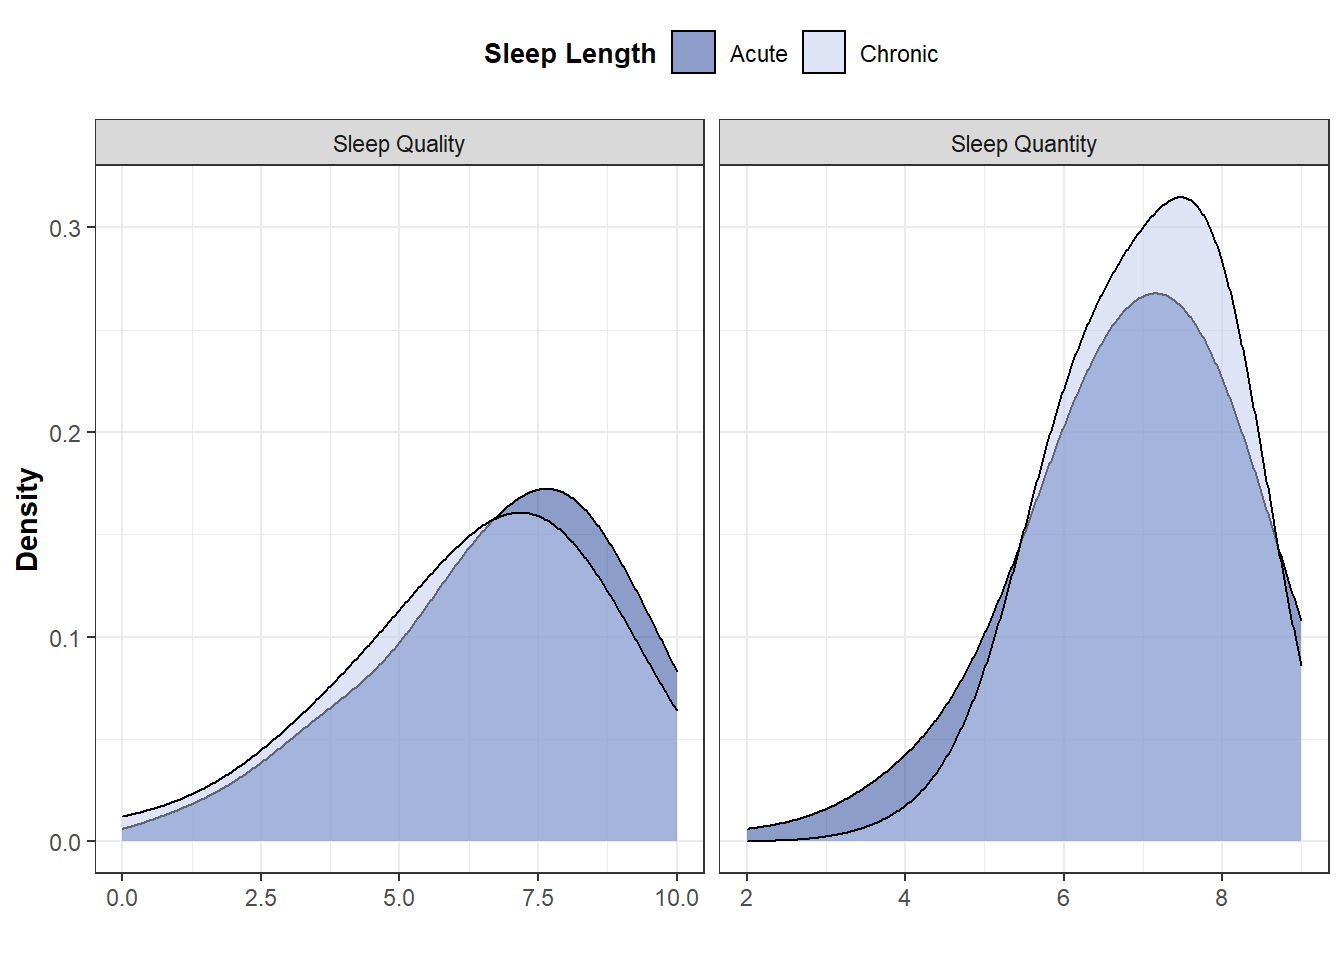
\includegraphics{SupplementaryCode_files/figure-latex/unnamed-chunk-25-1.pdf}

\hypertarget{study-3}{%
\chapter{Study 3}\label{study-3}}

\textbf{Load raw datasets}

\begin{Shaded}
\begin{Highlighting}[]
\NormalTok{Data_Study3_JEPG<-}\KeywordTok{read.delim}\NormalTok{(}\StringTok{"C:/Users/coren/Documents/JEPgeneral/SupplementaryCode/Data/Data-Study3-JEPG.txt"}\NormalTok{)}
\end{Highlighting}
\end{Shaded}

\hypertarget{filter-raw-data-based-upon-inclusion-criteria-1}{%
\section{Filter raw data based upon inclusion criteria}\label{filter-raw-data-based-upon-inclusion-criteria-1}}

\begin{Shaded}
\begin{Highlighting}[]
\NormalTok{Data_Study3_Raw<-}\StringTok{ }\NormalTok{Data_Study3_JEPG }\OperatorTok\StringTok{ }
\StringTok{  }\KeywordTok{mutate}\NormalTok{(}
\CommentTok{#Check for missing Data}
   \DataTypeTok{CCA=}\KeywordTok{case_when}\NormalTok{(}
      \KeywordTok{is.na}\NormalTok{(Moral_TOT) }\OperatorTok{|}\StringTok{ }\KeywordTok{is.na}\NormalTok{(SleepQualCro) }\OperatorTok{|}\StringTok{ }\KeywordTok{is.na}\NormalTok{(SleepQualAcu) }\OperatorTok{|}\StringTok{ }\KeywordTok{is.na}\NormalTok{(SleepQuantCro) }\OperatorTok{|}\StringTok{ }
\StringTok{        }\KeywordTok{is.na}\NormalTok{(SleepQuantAcu) }\OperatorTok{~}\DecValTok{0}\NormalTok{, }
      \OperatorTok{!}\KeywordTok{is.na}\NormalTok{(Moral_TOT) }\OperatorTok{|}\StringTok{ }\OperatorTok{!}\KeywordTok{is.na}\NormalTok{(SleepQualCro) }\OperatorTok{&}\StringTok{ }\OperatorTok{!}\KeywordTok{is.na}\NormalTok{(SleepQualAcu) }\OperatorTok{&}\StringTok{ }\OperatorTok{!}\KeywordTok{is.na}\NormalTok{(SleepQuantCro) }\OperatorTok{&}
\StringTok{        }\OperatorTok{!}\KeywordTok{is.na}\NormalTok{(SleepQuantAcu) }\OperatorTok{~}\DecValTok{1}\NormalTok{),}
\CommentTok{#Detect age outside targetted range   }
    \DataTypeTok{Age_correct=}\KeywordTok{case_when}\NormalTok{(}
\NormalTok{      Age}\OperatorTok{>=}\DecValTok{18} \OperatorTok{&}\StringTok{ }\NormalTok{Age}\OperatorTok{<=}\DecValTok{50} \OperatorTok{~}\StringTok{ }\DecValTok{1}\NormalTok{,}
\NormalTok{      Age}\OperatorTok{<}\DecValTok{18} \OperatorTok{|}\StringTok{ }\NormalTok{Age}\OperatorTok{>}\DecValTok{50} \OperatorTok{~}\StringTok{ }\DecValTok{0}\NormalTok{))}
\end{Highlighting}
\end{Shaded}

\textbf{Filtering participants not fullfiling these 3 criteria}

\begin{Shaded}
\begin{Highlighting}[]
\NormalTok{Data_Study3_Wide<-}\StringTok{ }\KeywordTok{subset}\NormalTok{(Data_Study3_Raw, Age_correct}\OperatorTok{==}\DecValTok{1} \OperatorTok{&}\StringTok{ }\NormalTok{CCA}\OperatorTok{==}\DecValTok{1}\NormalTok{)}
\end{Highlighting}
\end{Shaded}

\hypertarget{data-analysis-2}{%
\section{Data analysis}\label{data-analysis-2}}

\textbf{Run linear regressions for each sleep variable (IV) on endorsement of moral principles (DV)}

\begin{Shaded}
\begin{Highlighting}[]
\NormalTok{QualCroLMS3<-}\KeywordTok{lm}\NormalTok{(Moral_TOT}\OperatorTok{~}\NormalTok{SleepQualCro, Data_Study3_Wide)}
\NormalTok{QualAcuLMS3<-}\KeywordTok{lm}\NormalTok{(Moral_TOT}\OperatorTok{~}\NormalTok{SleepQualAcu,Data_Study3_Wide)}
\NormalTok{QuantCroLMS3<-}\KeywordTok{lm}\NormalTok{(Moral_TOT}\OperatorTok{~}\NormalTok{SleepQuantCro, Data_Study3_Wide)}
\NormalTok{QuantAcuLMS3<-}\KeywordTok{lm}\NormalTok{(Moral_TOT}\OperatorTok{~}\NormalTok{SleepQuantAcu, Data_Study3_Wide)}
\end{Highlighting}
\end{Shaded}

\textbf{Extract coefficients (unstandardized slopes, standard errors and p-values) from linear regression models }

\begin{Shaded}
\begin{Highlighting}[]
\CommentTok{#Chronic Sleep Quality}
\NormalTok{bQualCroS3<-}\KeywordTok{round}\NormalTok{(}\KeywordTok{summary}\NormalTok{(QualCroLMS3)}\OperatorTok{$}\NormalTok{coefficients[}\DecValTok{2}\NormalTok{,}\DecValTok{1}\NormalTok{], }\DataTypeTok{digit=}\DecValTok{2}\NormalTok{)}
\NormalTok{SEQualCroS3<-}\StringTok{ }\KeywordTok{round}\NormalTok{(}\KeywordTok{summary}\NormalTok{(QualCroLMS3)}\OperatorTok{$}\NormalTok{coefficients[}\DecValTok{2}\NormalTok{,}\DecValTok{2}\NormalTok{] , }\DataTypeTok{digit=}\DecValTok{2}\NormalTok{)}
\NormalTok{pQualCroS3<-}\StringTok{ }\KeywordTok{round}\NormalTok{(}\KeywordTok{ifelse}\NormalTok{(}\KeywordTok{summary}\NormalTok{(QualCroLMS3)}\OperatorTok{$}\NormalTok{coefficients[}\DecValTok{2}\NormalTok{,}\DecValTok{4}\NormalTok{]}\OperatorTok{*}\DecValTok{4}\OperatorTok{<}\NormalTok{.}\DecValTok{99}\NormalTok{, }\KeywordTok{summary}\NormalTok{(QualCroLMS3)}\OperatorTok{$}\NormalTok{coefficients[}\DecValTok{2}\NormalTok{,}\DecValTok{4}\NormalTok{]}\OperatorTok{*}\DecValTok{4}\NormalTok{, }\FloatTok{.99}\NormalTok{), }\DataTypeTok{digit=}\DecValTok{2}\NormalTok{)}

\CommentTok{#Acute Sleep Quality}
\NormalTok{bQualAcuS3<-}\StringTok{ }\KeywordTok{round}\NormalTok{(}\KeywordTok{summary}\NormalTok{(QualAcuLMS3)}\OperatorTok{$}\NormalTok{coefficients[}\DecValTok{2}\NormalTok{,}\DecValTok{1}\NormalTok{] , }\DataTypeTok{digit=}\DecValTok{2}\NormalTok{)}
\NormalTok{SEQualAcuS3 <-}\StringTok{ }\KeywordTok{round}\NormalTok{(}\KeywordTok{summary}\NormalTok{(QualAcuLMS3)}\OperatorTok{$}\NormalTok{coefficients[}\DecValTok{2}\NormalTok{,}\DecValTok{2}\NormalTok{] , }\DataTypeTok{digit=}\DecValTok{2}\NormalTok{)}
\NormalTok{pQualAcuS3<-}\StringTok{ }\KeywordTok{round}\NormalTok{(}\KeywordTok{ifelse}\NormalTok{(}\KeywordTok{summary}\NormalTok{(QualAcuLMS3)}\OperatorTok{$}\NormalTok{coefficients[}\DecValTok{2}\NormalTok{,}\DecValTok{4}\NormalTok{]}\OperatorTok{*}\DecValTok{4}\OperatorTok{<}\NormalTok{.}\DecValTok{99}\NormalTok{, }\KeywordTok{summary}\NormalTok{(QualAcuLMS3)}\OperatorTok{$}\NormalTok{coefficients[}\DecValTok{2}\NormalTok{,}\DecValTok{4}\NormalTok{]}\OperatorTok{*}\DecValTok{4}\NormalTok{, }\FloatTok{.99}\NormalTok{), }\DataTypeTok{digit=}\DecValTok{2}\NormalTok{)}

\CommentTok{#Chronic Sleep Quantity}
\NormalTok{bQuantCroS3<-}\StringTok{ }\KeywordTok{round}\NormalTok{(}\KeywordTok{summary}\NormalTok{(QuantCroLMS3)}\OperatorTok{$}\NormalTok{coefficients[}\DecValTok{2}\NormalTok{,}\DecValTok{1}\NormalTok{] , }\DataTypeTok{digit=}\DecValTok{2}\NormalTok{)}
\NormalTok{SEQuantCroS3 <-}\StringTok{ }\KeywordTok{round}\NormalTok{(}\KeywordTok{summary}\NormalTok{(QuantCroLMS3)}\OperatorTok{$}\NormalTok{coefficients[}\DecValTok{2}\NormalTok{,}\DecValTok{2}\NormalTok{] , }\DataTypeTok{digit=}\DecValTok{2}\NormalTok{)}
\NormalTok{pQuantCroS3<-}\StringTok{ }\KeywordTok{round}\NormalTok{(}\KeywordTok{ifelse}\NormalTok{(}\KeywordTok{summary}\NormalTok{(QuantCroLMS3)}\OperatorTok{$}\NormalTok{coefficients[}\DecValTok{2}\NormalTok{,}\DecValTok{4}\NormalTok{]}\OperatorTok{*}\DecValTok{4}\OperatorTok{<}\NormalTok{.}\DecValTok{99}\NormalTok{, }\KeywordTok{summary}\NormalTok{(QuantCroLMS3)}\OperatorTok{$}\NormalTok{coefficients[}\DecValTok{2}\NormalTok{,}\DecValTok{4}\NormalTok{]}\OperatorTok{*}\DecValTok{4}\NormalTok{, }\FloatTok{.99}\NormalTok{), }\DataTypeTok{digit=}\DecValTok{2}\NormalTok{)}

\CommentTok{#Acute Sleep Quantity}
\NormalTok{bQuantAcuS3<-}\StringTok{ }\KeywordTok{round}\NormalTok{(}\KeywordTok{summary}\NormalTok{(QuantAcuLMS3)}\OperatorTok{$}\NormalTok{coefficients[}\DecValTok{2}\NormalTok{,}\DecValTok{1}\NormalTok{] , }\DataTypeTok{digit=}\DecValTok{2}\NormalTok{)}
\NormalTok{SEQuantAcuS3 <-}\StringTok{ }\KeywordTok{round}\NormalTok{(}\KeywordTok{summary}\NormalTok{(QuantAcuLMS3)}\OperatorTok{$}\NormalTok{coefficients[}\DecValTok{2}\NormalTok{,}\DecValTok{2}\NormalTok{] , }\DataTypeTok{digit=}\DecValTok{2}\NormalTok{)}
\NormalTok{pQuantAcuS3<-}\StringTok{ }\KeywordTok{round}\NormalTok{(}\KeywordTok{ifelse}\NormalTok{(}\KeywordTok{summary}\NormalTok{(QuantAcuLMS3)}\OperatorTok{$}\NormalTok{coefficients[}\DecValTok{2}\NormalTok{,}\DecValTok{4}\NormalTok{]}\OperatorTok{*}\DecValTok{4}\OperatorTok{<}\NormalTok{.}\DecValTok{99}\NormalTok{, }\KeywordTok{summary}\NormalTok{(QuantAcuLMS3)}\OperatorTok{$}\NormalTok{coefficients[}\DecValTok{2}\NormalTok{,}\DecValTok{4}\NormalTok{]}\OperatorTok{*}\DecValTok{4}\NormalTok{, }\FloatTok{.99}\NormalTok{), }\DataTypeTok{digit=}\DecValTok{2}\NormalTok{)}
\end{Highlighting}
\end{Shaded}

\textbf{Put results in a table}

\begin{Shaded}
\begin{Highlighting}[]
\NormalTok{SleepMarker<-}\KeywordTok{c}\NormalTok{(}\StringTok{"Quality Chronic"}\NormalTok{,}\StringTok{"Quality Acute"}\NormalTok{,}\StringTok{"Quantity Chronic"}\NormalTok{,}\StringTok{"Quantity Acute"}\NormalTok{)}
\NormalTok{bS3<-}\KeywordTok{c}\NormalTok{(bQualCroS3,bQualAcuS3,bQuantCroS3,bQuantAcuS3)}
\NormalTok{SES3<-}\KeywordTok{c}\NormalTok{(SEQualCroS3,SEQualAcuS3,SEQuantCroS3,SEQuantAcuS3)}
\NormalTok{pvalS3<-}\KeywordTok{c}\NormalTok{(pQualCroS3,pQualAcuS3,pQuantCroS3,pQuantAcuS3)}
\NormalTok{NS3<-}\KeywordTok{c}\NormalTok{(}\KeywordTok{length}\NormalTok{(QualCroLMS3}\OperatorTok{$}\NormalTok{fitted.values),}
     \KeywordTok{length}\NormalTok{(QualAcuLMS3}\OperatorTok{$}\NormalTok{fitted.values),}
     \KeywordTok{length}\NormalTok{(QuantCroLMS3}\OperatorTok{$}\NormalTok{fitted.values),}
     \KeywordTok{length}\NormalTok{(QuantAcuLMS3}\OperatorTok{$}\NormalTok{fitted.values))}
\NormalTok{ResultsStudy3<-}\KeywordTok{data.frame}\NormalTok{(}\StringTok{"Sleep Indicator"}\NormalTok{=SleepMarker, }\StringTok{"Unstandardized Slope"}\NormalTok{=bS3, }\StringTok{"Standard Errors"}\NormalTok{=SES3, }\StringTok{"p values"}\NormalTok{=pvalS3, }\StringTok{"N"}\NormalTok{=NS3)}
\KeywordTok{gt}\NormalTok{(ResultsStudy3)}
\end{Highlighting}
\end{Shaded}

\captionsetup[table]{labelformat=empty,skip=1pt}
\begin{longtable}{crrrc}
\toprule
Sleep.Indicator & Unstandardized.Slope & Standard.Errors & p.values & N \\ 
\midrule
Quality Chronic & 0.24 & 0.25 & 0.99 & 55 \\ 
Quality Acute & 0.09 & 0.23 & 0.99 & 55 \\ 
Quantity Chronic & 0.07 & 0.27 & 0.99 & 55 \\ 
Quantity Acute & -0.07 & 0.25 & 0.99 & 55 \\ 
\bottomrule
\end{longtable}

\textbf{Create datasets to display regression summary on the plots}

\begin{Shaded}
\begin{Highlighting}[]
\NormalTok{ResumQualCroS3<-}\StringTok{ }\KeywordTok{paste0}\NormalTok{(}\StringTok{"b="}\NormalTok{,bQualCroS3,}\StringTok{", "}\NormalTok{, }\StringTok{"SE="}\NormalTok{,SEQualCroS3,}\StringTok{", "}\NormalTok{,}\StringTok{"p="}\NormalTok{,pQualCroS3)}
\NormalTok{ResumQualAcuS3<-}\StringTok{ }\KeywordTok{paste0}\NormalTok{(}\StringTok{"b="}\NormalTok{,bQualAcuS3,}\StringTok{", "}\NormalTok{, }\StringTok{"SE="}\NormalTok{,SEQualAcuS3,}\StringTok{", "}\NormalTok{,}\StringTok{"p="}\NormalTok{,pQualAcuS3)}
\NormalTok{ResumQuantCroS3<-}\StringTok{ }\KeywordTok{paste0}\NormalTok{(}\StringTok{"b="}\NormalTok{,bQuantCroS3,}\StringTok{", "}\NormalTok{, }\StringTok{"SE="}\NormalTok{,SEQuantCroS3,}\StringTok{", "}\NormalTok{,}\StringTok{"p="}\NormalTok{,pQuantCroS3)}
\NormalTok{ResumQuantAcuS3<-}\StringTok{ }\KeywordTok{paste0}\NormalTok{(}\StringTok{"b="}\NormalTok{,bQuantAcuS3,}\StringTok{", "}\NormalTok{, }\StringTok{"SE="}\NormalTok{,SEQuantAcuS3,}\StringTok{", "}\NormalTok{,}\StringTok{"p="}\NormalTok{,pQuantAcuS3)}

\NormalTok{annotationQualCroS3 <-}\StringTok{ }\KeywordTok{data.frame}\NormalTok{(}\DataTypeTok{x =} \DecValTok{5}\NormalTok{, }\DataTypeTok{y =} \DecValTok{43}\NormalTok{,  }\DataTypeTok{label =}\NormalTok{ ResumQualCroS3)}
\NormalTok{annotationQualAcuS3 <-}\StringTok{ }\KeywordTok{data.frame}\NormalTok{(}\DataTypeTok{x =} \DecValTok{5}\NormalTok{, }\DataTypeTok{y =} \DecValTok{43}\NormalTok{,  }\DataTypeTok{label =}\NormalTok{ ResumQualAcuS3)}
\NormalTok{annotationQuantCroS3 <-}\StringTok{ }\KeywordTok{data.frame}\NormalTok{(}\DataTypeTok{x =}\DecValTok{5}\NormalTok{, }\DataTypeTok{y =} \DecValTok{43}\NormalTok{,  }\DataTypeTok{label =}\NormalTok{ ResumQuantCroS3)}
\NormalTok{annotationQuantAcuS3 <-}\StringTok{ }\KeywordTok{data.frame}\NormalTok{(}\DataTypeTok{x =} \DecValTok{5}\NormalTok{, }\DataTypeTok{y =} \DecValTok{43}\NormalTok{,  }\DataTypeTok{label =}\NormalTok{ ResumQuantAcuS3)}

\NormalTok{annotationS3<-}\KeywordTok{cbind}\NormalTok{(}
  \KeywordTok{rbind}\NormalTok{(annotationQualCroS3, }
\NormalTok{        annotationQualAcuS3, }
\NormalTok{        annotationQuantCroS3, }
\NormalTok{        annotationQuantAcuS3),}
  \DataTypeTok{SleepType=}\KeywordTok{c}\NormalTok{(}
        \StringTok{"Quality of Chronic Sleep"}\NormalTok{, }
        \StringTok{"Quality of Acute Sleep"}\NormalTok{, }
        \StringTok{"Quantity of Chronic Sleep"}\NormalTok{, }
        \StringTok{"Quantity of Acute Sleep"}\NormalTok{))}
\end{Highlighting}
\end{Shaded}

\textbf{Prepare data for plots}

\begin{Shaded}
\begin{Highlighting}[]
\NormalTok{Data_PlotS3<-}\StringTok{ }\NormalTok{Data_Study3_Wide }\OperatorTok
\StringTok{  }\KeywordTok{pivot_longer}\NormalTok{(}
    \DataTypeTok{cols=}\KeywordTok{c}\NormalTok{(SleepQualCro, SleepQualAcu, SleepQuantCro, SleepQuantAcu),}
    \DataTypeTok{names_to=}\StringTok{"SleepType"}\NormalTok{) }\OperatorTok
\StringTok{  }\KeywordTok{rename}\NormalTok{(}\StringTok{"SleepValue"}\NormalTok{=value) }\OperatorTok
\StringTok{  }\KeywordTok{mutate}\NormalTok{(}
    \DataTypeTok{SleepLength=}\KeywordTok{case_when}\NormalTok{(}
\NormalTok{      SleepType}\OperatorTok{==}\StringTok{"SleepQualCro"} \OperatorTok{|}\StringTok{ }\NormalTok{SleepType}\OperatorTok{==}\StringTok{"SleepQuantCro"}\OperatorTok{~}\StringTok{"Chronic"}\NormalTok{,}
\NormalTok{      SleepType}\OperatorTok{==}\StringTok{"SleepQualAcu"} \OperatorTok{|}\StringTok{ }\NormalTok{SleepType}\OperatorTok{==}\StringTok{"SleepQuantAcu"}\OperatorTok{~}\StringTok{"Acute"}\NormalTok{),}
    \DataTypeTok{SleepQuanthist=}\KeywordTok{case_when}\NormalTok{(}
\NormalTok{      SleepType}\OperatorTok{==}\StringTok{"SleepQualCro"} \OperatorTok{|}\StringTok{ }\NormalTok{SleepType}\OperatorTok{==}\StringTok{"SleepQualAcu"}\OperatorTok{~}\StringTok{"Sleep Quality"}\NormalTok{,}
\NormalTok{      SleepType}\OperatorTok{==}\StringTok{"SleepQuantCro"} \OperatorTok{|}\StringTok{ }\NormalTok{SleepType}\OperatorTok{==}\StringTok{"SleepQuantAcu"}\OperatorTok{~}\StringTok{"Sleep Quantity"}\NormalTok{))}

\NormalTok{Data_PlotS3}\OperatorTok{$}\NormalTok{SleepType<-dplyr}\OperatorTok{::}\KeywordTok{recode}\NormalTok{(Data_PlotS3}\OperatorTok{$}\NormalTok{SleepType, }
        \StringTok{"SleepQualCro"}\NormalTok{ =}\StringTok{ "Quality of Chronic Sleep"}\NormalTok{,}
        \StringTok{"SleepQualAcu"}\NormalTok{ =}\StringTok{ "Quality of Acute Sleep"}\NormalTok{,}
        \StringTok{"SleepQuantCro"}\NormalTok{ =}\StringTok{ "Quantity of Chronic Sleep"}\NormalTok{,}
        \StringTok{"SleepQuantAcu"}\NormalTok{ =}\StringTok{ "Quantity of Acute Sleep"}\NormalTok{)}
\end{Highlighting}
\end{Shaded}

\textbf{Plot distribution of each sleep indicator}

\begin{Shaded}
\begin{Highlighting}[]
\NormalTok{DistQualityS3<-}\KeywordTok{ggplot}\NormalTok{(Data_PlotS3, }\KeywordTok{aes}\NormalTok{(}\DataTypeTok{x=}\NormalTok{SleepValue, }\DataTypeTok{fill=}\KeywordTok{factor}\NormalTok{(SleepLength))) }\OperatorTok{+}\StringTok{ }
\StringTok{  }\KeywordTok{geom_density}\NormalTok{(}\DataTypeTok{alpha=}\FloatTok{0.5}\NormalTok{, }\DataTypeTok{size=}\FloatTok{0.5}\NormalTok{,}\DataTypeTok{adjust =} \DecValTok{2}\NormalTok{) }\OperatorTok{+}\StringTok{ }
\StringTok{  }\KeywordTok{scale_fill_manual}\NormalTok{(}\DataTypeTok{values=}\KeywordTok{c}\NormalTok{(}\StringTok{"#193B94"}\NormalTok{, }\StringTok{"#BDCAEE"}\NormalTok{, }\StringTok{"#193B94"}\NormalTok{, }\StringTok{"#BDCAEE"}\NormalTok{)) }\OperatorTok{+}
\StringTok{  }\KeywordTok{theme_bw}\NormalTok{() }\OperatorTok{+}\StringTok{ }
\StringTok{  }\KeywordTok{ylab}\NormalTok{(}\StringTok{"Density"}\NormalTok{) }\OperatorTok{+}\StringTok{ }\KeywordTok{xlab}\NormalTok{(}\StringTok{""}\NormalTok{) }\OperatorTok{+}
\StringTok{  }\KeywordTok{facet_wrap}\NormalTok{(}\OperatorTok{~}\KeywordTok{factor}\NormalTok{(SleepQuanthist), }\DataTypeTok{scale=}\StringTok{"free_x"}\NormalTok{) }\OperatorTok{+}\StringTok{ }
\StringTok{  }\KeywordTok{guides}\NormalTok{(}\DataTypeTok{fill=}\KeywordTok{guide_legend}\NormalTok{(}\StringTok{"Sleep Length"}\NormalTok{)) }\OperatorTok{+}
\StringTok{  }\KeywordTok{theme}\NormalTok{(}
    \DataTypeTok{axis.title.y =} \KeywordTok{element_text}\NormalTok{(}\DataTypeTok{size =} \DecValTok{11}\NormalTok{, }\DataTypeTok{hjust =} \FloatTok{0.5}\NormalTok{, }\DataTypeTok{face=}\StringTok{"bold"}\NormalTok{),}
    \DataTypeTok{axis.title.x =} \KeywordTok{element_text}\NormalTok{(}\DataTypeTok{face=}\StringTok{"bold"}\NormalTok{, }\DataTypeTok{size =} \DecValTok{11}\NormalTok{, }\DataTypeTok{hjust =} \FloatTok{0.5}\NormalTok{),}
    \DataTypeTok{legend.position=}\StringTok{"top"}\NormalTok{,}
    \DataTypeTok{legend.title =} \KeywordTok{element_text}\NormalTok{(}\DataTypeTok{colour=}\StringTok{"black"}\NormalTok{, }\DataTypeTok{size=}\DecValTok{10}\NormalTok{, }\DataTypeTok{face=}\StringTok{"bold"}\NormalTok{)) }
\NormalTok{DistQualityS3}
\end{Highlighting}
\end{Shaded}

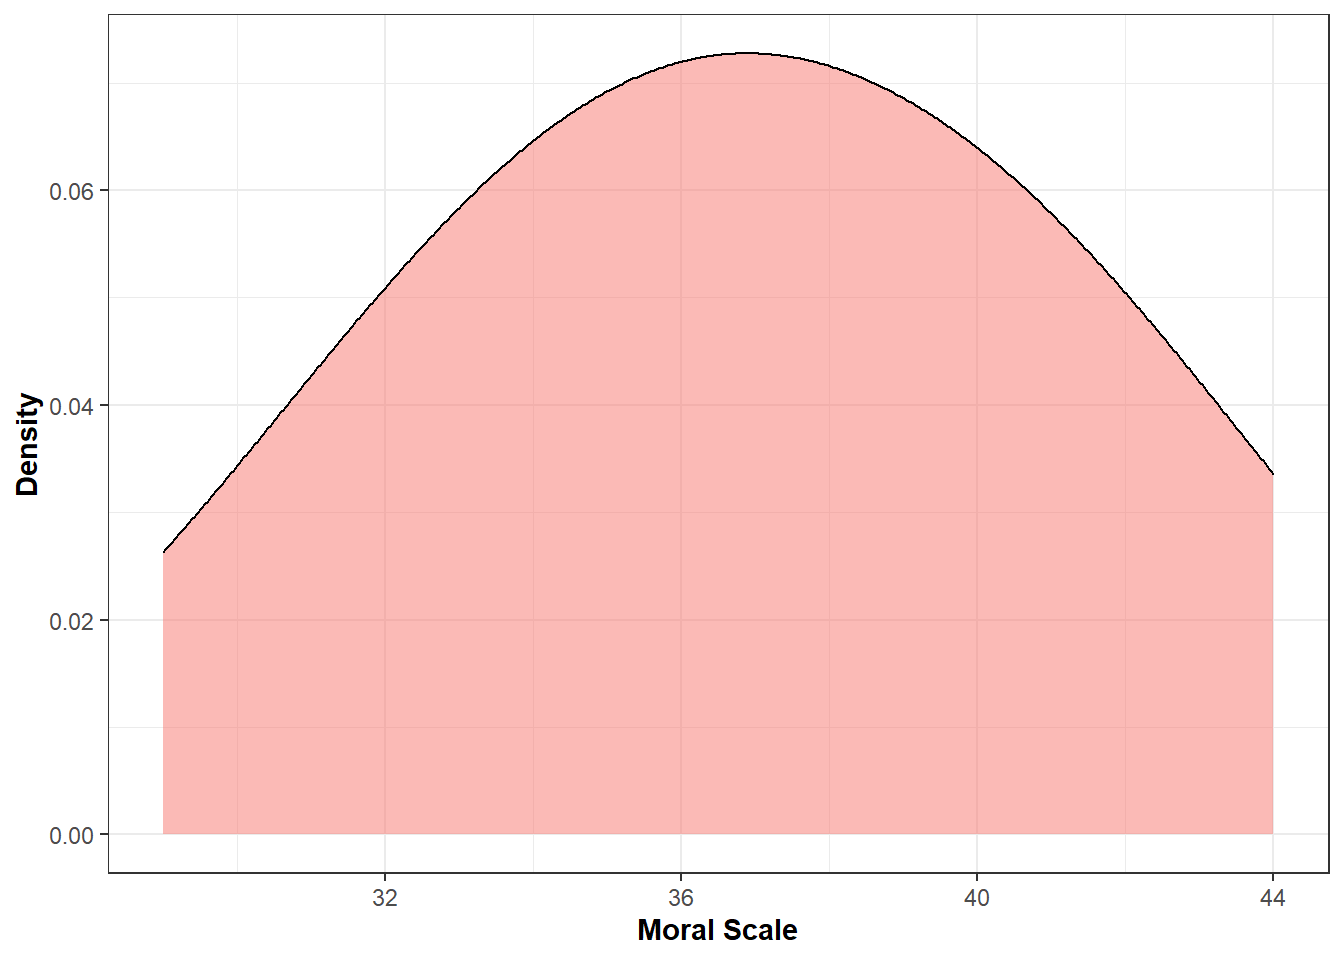
\includegraphics{SupplementaryCode_files/figure-latex/unnamed-chunk-34-1.pdf}

\textbf{N in each sleep quantity category}

\begin{Shaded}
\begin{Highlighting}[]
\NormalTok{Dist.Quantity.ChronicS3<-Data_Study3_Wide }\OperatorTok\StringTok{ }
\StringTok{    }\NormalTok{dplyr}\OperatorTok{::}\KeywordTok{group_by}\NormalTok{(SleepQuantCro) }\OperatorTok\StringTok{ }
\StringTok{      }\KeywordTok{summarise}\NormalTok{(}
        \DataTypeTok{N=}\KeywordTok{n}\NormalTok{()) }\OperatorTok\StringTok{ }
\StringTok{          }\KeywordTok{spread}\NormalTok{(SleepQuantCro, N) }\OperatorTok\StringTok{ }
\StringTok{  }\KeywordTok{as.data.frame}\NormalTok{()}
\KeywordTok{row.names}\NormalTok{(Dist.Quantity.ChronicS3)<-}\StringTok{"Quantity Chronic"}

\NormalTok{Dist.Quantity.AcuteS3<-Data_Study3_Wide }\OperatorTok\StringTok{ }
\StringTok{    }\NormalTok{dplyr}\OperatorTok{::}\KeywordTok{group_by}\NormalTok{(SleepQuantAcu) }\OperatorTok\StringTok{ }
\StringTok{      }\KeywordTok{summarise}\NormalTok{(}
        \DataTypeTok{N=}\KeywordTok{n}\NormalTok{()) }\OperatorTok\StringTok{ }
\StringTok{          }\KeywordTok{spread}\NormalTok{(SleepQuantAcu, N) }\OperatorTok\StringTok{ }
\StringTok{  }\KeywordTok{as.data.frame}\NormalTok{()}
\KeywordTok{row.names}\NormalTok{(Dist.Quantity.AcuteS3)<-}\StringTok{"Quantity Acute"}

\KeywordTok{bind_rows}\NormalTok{(Dist.Quantity.AcuteS3, Dist.Quantity.ChronicS3)}
\end{Highlighting}
\end{Shaded}

\begin{verbatim}
##                  0  2 4 5  6  7  8 9 10 12  1
## Quantity Acute   2  1 2 5 10 14  8 8  4  1 NA
## Quantity Chronic 2 NA 2 5 12 10 13 8  2 NA  1
\end{verbatim}

\textbf{Scatterplots}

\begin{Shaded}
\begin{Highlighting}[]
\KeywordTok{ggplot}\NormalTok{(Data_PlotS3, }\KeywordTok{aes}\NormalTok{(}\DataTypeTok{x=}\NormalTok{SleepValue, }\DataTypeTok{y=}\NormalTok{Moral_TOT)) }\OperatorTok{+}\StringTok{ }
\StringTok{       }\KeywordTok{geom_jitter}\NormalTok{(}\DataTypeTok{alpha=}\FloatTok{0.6}\NormalTok{, }\DataTypeTok{color=}\StringTok{"#545454"}\NormalTok{, }\DataTypeTok{size=}\FloatTok{1.2}\NormalTok{) }\OperatorTok{+}\StringTok{ }
\StringTok{       }\CommentTok{# geom_line(aes(y= fit), colour="#0019D0", size=1.2) + }
\StringTok{       }\CommentTok{# geom_ribbon( aes(ymin = lwr, ymax = upr), fill = "#697BFC", alpha = .3)+}
\StringTok{       }\KeywordTok{geom_smooth}\NormalTok{(}\DataTypeTok{method=}\StringTok{"lm"}\NormalTok{)}\OperatorTok{+}
\StringTok{       }\KeywordTok{facet_wrap}\NormalTok{(}\OperatorTok{~}\KeywordTok{factor}\NormalTok{(SleepType), }\DataTypeTok{scales=}\StringTok{"free_x"}\NormalTok{) }\OperatorTok{+}
\StringTok{       }\KeywordTok{theme_bw}\NormalTok{() }\OperatorTok{+}\StringTok{ }\KeywordTok{ylab}\NormalTok{(}\StringTok{"Utilitirianism"}\NormalTok{) }\OperatorTok{+}\StringTok{ }\KeywordTok{xlab}\NormalTok{(}\StringTok{""}\NormalTok{) }\OperatorTok{+}\StringTok{ }
\StringTok{       }\KeywordTok{theme}\NormalTok{(}\DataTypeTok{axis.title.y =} \KeywordTok{element_text}\NormalTok{(}\DataTypeTok{size =} \DecValTok{11}\NormalTok{, }\DataTypeTok{hjust =} \FloatTok{0.5}\NormalTok{, }\DataTypeTok{face=}\StringTok{"bold"}\NormalTok{), }
             \DataTypeTok{axis.title.x =} \KeywordTok{element_text}\NormalTok{(}\DataTypeTok{face=}\StringTok{"bold"}\NormalTok{, }\DataTypeTok{size =} \DecValTok{11}\NormalTok{, }\DataTypeTok{hjust =} \FloatTok{0.5}\NormalTok{)) }\OperatorTok{+}
\StringTok{       }\KeywordTok{guides}\NormalTok{(}\DataTypeTok{size=}\OtherTok{FALSE}\NormalTok{, }\DataTypeTok{colour=}\OtherTok{FALSE}\NormalTok{, }\DataTypeTok{fill=}\OtherTok{FALSE}\NormalTok{) }\OperatorTok{+}\StringTok{ }
\StringTok{       }\KeywordTok{geom_label}\NormalTok{(}\DataTypeTok{data=}\NormalTok{annotationS3, }\KeywordTok{aes}\NormalTok{( }\DataTypeTok{x=}\NormalTok{x, }\DataTypeTok{y=}\NormalTok{y, }\DataTypeTok{label=}\NormalTok{label), }
                  \DataTypeTok{color=}\StringTok{"black"}\NormalTok{,  }\DataTypeTok{size=}\FloatTok{3.5}\NormalTok{ , }\DataTypeTok{angle=}\DecValTok{45}\NormalTok{, }\DataTypeTok{alpha=}\DecValTok{7}\OperatorTok{/}\DecValTok{10}\NormalTok{, }\DataTypeTok{inherit.aes =} \OtherTok{FALSE}\NormalTok{)}
\end{Highlighting}
\end{Shaded}

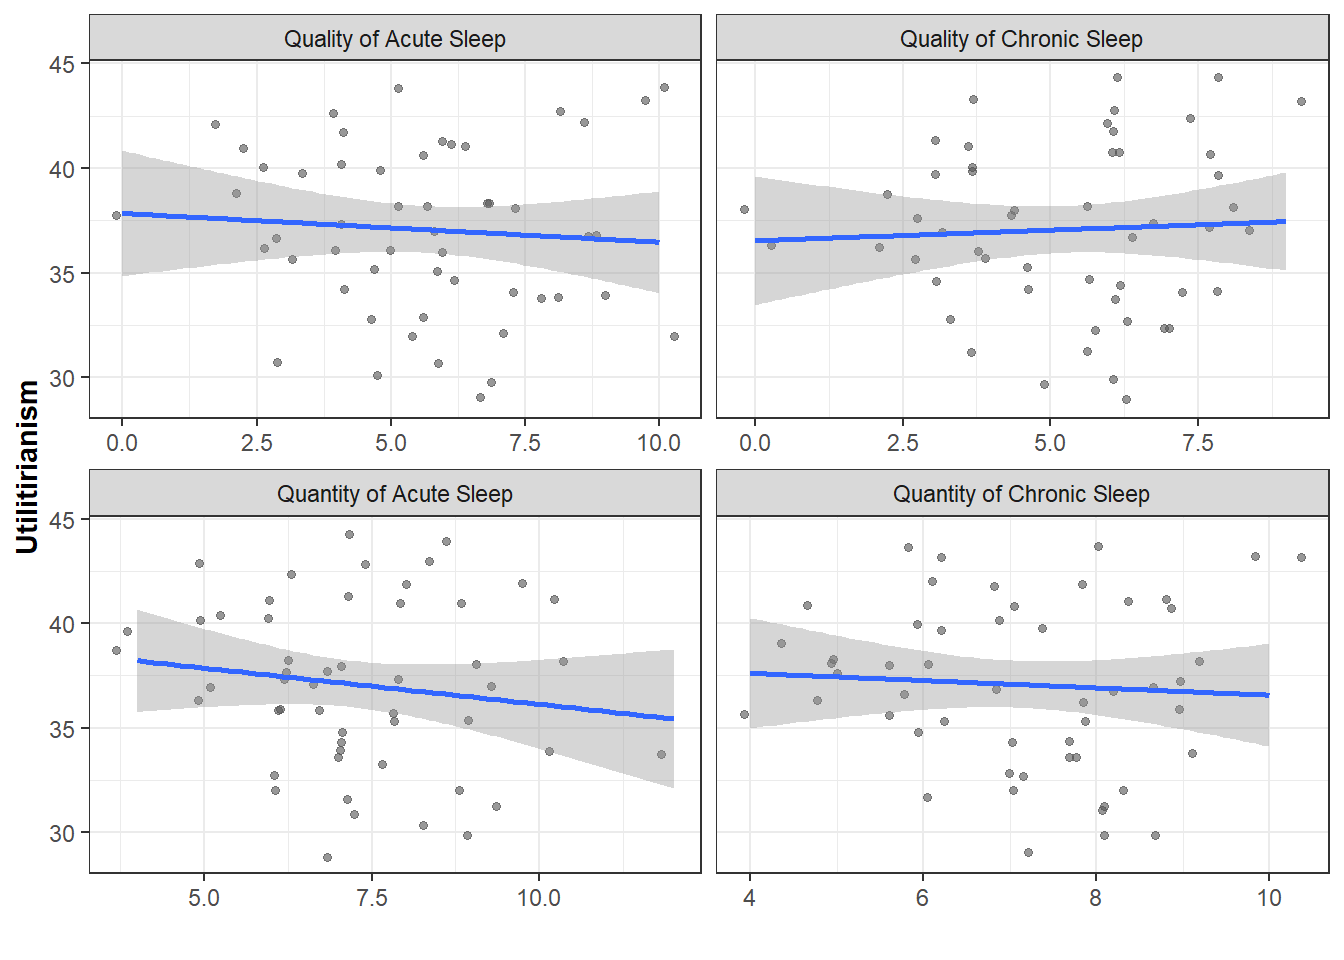
\includegraphics{SupplementaryCode_files/figure-latex/unnamed-chunk-36-1.pdf}

\hypertarget{study-4}{%
\chapter{Study 4}\label{study-4}}

\begin{Shaded}
\begin{Highlighting}[]
\KeywordTok{library}\NormalTok{(knitr);}\KeywordTok{library}\NormalTok{(geepack); }\KeywordTok{library}\NormalTok{(gt); }\KeywordTok{library}\NormalTok{(ggplot2); }\KeywordTok{library}\NormalTok{(readxl);  }\KeywordTok{library}\NormalTok{(tidyr); }\KeywordTok{library}\NormalTok{(dplyr); }\KeywordTok{library}\NormalTok{(rmdformats);  }\KeywordTok{library}\NormalTok{(car);}\KeywordTok{library}\NormalTok{(lavaan)}
\end{Highlighting}
\end{Shaded}

\textbf{Load raw datasets}

\begin{Shaded}
\begin{Highlighting}[]
\NormalTok{Data_Study4_JEPG<-}\KeywordTok{read.delim}\NormalTok{(}\StringTok{"C:/Users/coren/Documents/JEPgeneral/SupplementaryCode/Data/Data-Study4-JEPG.txt"}\NormalTok{)}
\end{Highlighting}
\end{Shaded}

\hypertarget{filter-raw-data-based-upon-inclusion-criteria-missing-data-1}{%
\section{Filter raw data based upon inclusion criteria \& missing data}\label{filter-raw-data-based-upon-inclusion-criteria-missing-data-1}}

\begin{Shaded}
\begin{Highlighting}[]
\NormalTok{Data_Study4_Raw<-}\StringTok{ }\NormalTok{Data_Study4_JEPG }\OperatorTok
\StringTok{  }\KeywordTok{mutate}\NormalTok{(}
\CommentTok{#Check for missing Data}
   \DataTypeTok{CCA=}\KeywordTok{case_when}\NormalTok{(}
      \KeywordTok{is.na}\NormalTok{(Moral_DIL) }\OperatorTok{|}\KeywordTok{is.na}\NormalTok{(Moral_SCA) }\OperatorTok{|}\StringTok{ }\KeywordTok{is.na}\NormalTok{(Moral_CAR) }\OperatorTok{|}\StringTok{ }\KeywordTok{is.na}\NormalTok{(SleepQualCro) }\OperatorTok{|}\StringTok{ }\KeywordTok{is.na}\NormalTok{(SleepQualAcu)  }\OperatorTok{|}\StringTok{ }\KeywordTok{is.na}\NormalTok{(SleepQuantCro) }\OperatorTok{|}\StringTok{ }\KeywordTok{is.na}\NormalTok{(SleepQuantAcu) }\OperatorTok{~}\DecValTok{0}\NormalTok{,}
      \OperatorTok{!}\KeywordTok{is.na}\NormalTok{(Moral_DIL) }\OperatorTok{&}\StringTok{ }\OperatorTok{!}\KeywordTok{is.na}\NormalTok{(Moral_SCA) }\OperatorTok{&}\StringTok{ }\OperatorTok{!}\KeywordTok{is.na}\NormalTok{(Moral_CAR) }\OperatorTok{&}\StringTok{ }\OperatorTok{!}\KeywordTok{is.na}\NormalTok{(SleepQualCro)}
      \OperatorTok{&}\StringTok{ }\OperatorTok{!}\KeywordTok{is.na}\NormalTok{(SleepQualAcu) }\OperatorTok{&}\StringTok{ }\OperatorTok{!}\KeywordTok{is.na}\NormalTok{(SleepQuantCro) }\OperatorTok{&}\StringTok{ }\OperatorTok{!}\KeywordTok{is.na}\NormalTok{(SleepQuantAcu) }\OperatorTok{~}\DecValTok{1}\NormalTok{),}
\CommentTok{#Detect age outside targetted range}
    \DataTypeTok{Age_correct=}\KeywordTok{case_when}\NormalTok{(}
\NormalTok{      Age}\OperatorTok{>=}\DecValTok{18} \OperatorTok{&}\StringTok{ }\NormalTok{Age}\OperatorTok{<=}\DecValTok{50} \OperatorTok{~}\StringTok{ }\DecValTok{1}\NormalTok{,}
\NormalTok{      Age}\OperatorTok{<}\DecValTok{18} \OperatorTok{|}\StringTok{ }\NormalTok{Age}\OperatorTok{>}\DecValTok{50} \OperatorTok{~}\StringTok{ }\DecValTok{0}\NormalTok{),}
\CommentTok{#Detect participants failing at attention check}
    \DataTypeTok{Attention_check=}\KeywordTok{case_when}\NormalTok{(}
\NormalTok{      Tromp }\OperatorTok{==}\StringTok{ }\DecValTok{0}  \OperatorTok{~}\StringTok{ }\DecValTok{1}\NormalTok{,}
\NormalTok{      Tromp }\OperatorTok{==}\StringTok{ }\DecValTok{1} \OperatorTok{~}\StringTok{ }\DecValTok{0}\NormalTok{))}
\end{Highlighting}
\end{Shaded}

\textbf{Filtering participants not fullfiling these 3 criteria}

\begin{Shaded}
\begin{Highlighting}[]
\NormalTok{Data_Study4_Wide<-}\StringTok{ }\KeywordTok{subset}\NormalTok{(Data_Study4_Raw, Data_Study4_Raw}\OperatorTok{$}\NormalTok{CCA}\OperatorTok{==}\DecValTok{1} \OperatorTok{&}\StringTok{ }\NormalTok{Data_Study4_Raw}\OperatorTok{$}\NormalTok{Age_correct}\OperatorTok{==}\DecValTok{1} \OperatorTok{&}\StringTok{ }\NormalTok{Data_Study4_Raw}\OperatorTok{$}\NormalTok{Attention_check}\OperatorTok{==}\DecValTok{1}\NormalTok{)}
\NormalTok{Data_Study4_Wide}\OperatorTok{$}\NormalTok{Moral_DIL.lavaan<-Data_Study4_Wide}\OperatorTok{$}\NormalTok{Moral_DIL}\OperatorTok{/}\DecValTok{11}
\NormalTok{Data_Study4_Wide}\OperatorTok{$}\NormalTok{Moral_SCA.lavaan<-Data_Study4_Wide}\OperatorTok{$}\NormalTok{Moral_SCA}\OperatorTok{/}\DecValTok{13}
\end{Highlighting}
\end{Shaded}

\hypertarget{data-analysis-3}{%
\section{Data analysis}\label{data-analysis-3}}

\textbf{Planned statistical analysis: Run SEM for each sleep variable (IV) on endorsement of moral principles (DV)}

\begin{Shaded}
\begin{Highlighting}[]
\CommentTok{#Primary Analysis}
\NormalTok{Model_QualCroSEMS4<-}
\StringTok{'MoralTOT=~Moral_DIL.lavaan+Moral_SCA.lavaan+Moral_CAR}
\StringTok{MoralTOT~SleepQualCro'}
\NormalTok{fitQualCro<-}\KeywordTok{sem}\NormalTok{(Model_QualCroSEMS4, }\DataTypeTok{data=}\NormalTok{Data_Study4_Wide, }\DataTypeTok{estimator=}\StringTok{"MLR"}\NormalTok{)}

\CommentTok{#Secondary Analyses}
\NormalTok{Model_QualAcuSEMS4<-}
\StringTok{'MoralTOT=~Moral_DIL.lavaan+Moral_SCA.lavaan+Moral_CAR}
\StringTok{MoralTOT~SleepQualAcu'}
\NormalTok{fitQualAcu<-}\KeywordTok{sem}\NormalTok{(Model_QualAcuSEMS4, }\DataTypeTok{data=}\NormalTok{Data_Study4_Wide, }\DataTypeTok{estimator=}\StringTok{"MLR"}\NormalTok{)}


\NormalTok{Model_QuantCroSEMS4<-}
\StringTok{'MoralTOT=~Moral_DIL.lavaan+Moral_SCA.lavaan+Moral_CAR}
\StringTok{MoralTOT~SleepQuantCro'}
\NormalTok{fitQuantCro<-}\KeywordTok{sem}\NormalTok{(Model_QuantCroSEMS4, }\DataTypeTok{data=}\NormalTok{Data_Study4_Wide, }\DataTypeTok{estimator=}\StringTok{"MLR"}\NormalTok{)}


\NormalTok{Model_QuantAcuSEMS4<-}
\StringTok{'MoralTOT=~Moral_DIL.lavaan+Moral_SCA.lavaan+Moral_CAR}
\StringTok{MoralTOT~SleepQuantAcu'}
\NormalTok{fitQuantAcu<-}\KeywordTok{sem}\NormalTok{(Model_QuantAcuSEMS4, }\DataTypeTok{data=}\NormalTok{Data_Study4_Wide, }\DataTypeTok{estimator=}\StringTok{"MLR"}\NormalTok{)}


\KeywordTok{summary}\NormalTok{(fitQualCro)}
\end{Highlighting}
\end{Shaded}

\begin{verbatim}
## lavaan 0.6-6 did NOT end normally after 4707 iterations
## ** WARNING ** Estimates below are most likely unreliable
## 
##   Estimator                                         ML
##   Optimization method                           NLMINB
##   Number of free parameters                          7
##                                                       
##   Number of observations                            99
##                                                       
## Model Test User Model:
##                                                       
##   Test statistic                                    NA
##   Degrees of freedom                                NA
## 
## Parameter Estimates:
## 
##   Standard errors                             Sandwich
##   Information bread                           Observed
##   Observed information based on                Hessian
## 
## Latent Variables:
##                    Estimate  Std.Err  z-value  P(>|z|)
##   MoralTOT =~                                         
##     Moral_DIL.lavn    1.000                           
##     Moral_SCA.lavn   86.921       NA                  
##     Moral_CAR         0.029       NA                  
## 
## Regressions:
##                    Estimate  Std.Err  z-value  P(>|z|)
##   MoralTOT ~                                          
##     SleepQualCro      0.000       NA                  
## 
## Variances:
##                    Estimate  Std.Err  z-value  P(>|z|)
##    .Moral_DIL.lavn    5.503       NA                  
##    .Moral_SCA.lavn  -35.483       NA                  
##    .Moral_CAR         0.034       NA                  
##    .MoralTOT          0.005       NA
\end{verbatim}

\begin{Shaded}
\begin{Highlighting}[]
\KeywordTok{summary}\NormalTok{(fitQualAcu)}
\end{Highlighting}
\end{Shaded}

\begin{verbatim}
## lavaan 0.6-6 ended normally after 50 iterations
## 
##   Estimator                                         ML
##   Optimization method                           NLMINB
##   Number of free parameters                          7
##                                                       
##   Number of observations                            99
##                                                       
## Model Test User Model:
##                                                Standard      Robust
##   Test Statistic                                  0.061       0.056
##   Degrees of freedom                                  2           2
##   P-value (Chi-square)                            0.970       0.972
##   Scaling correction factor                                   1.093
##        Yuan-Bentler correction (Mplus variant)                     
## 
## Parameter Estimates:
## 
##   Standard errors                             Sandwich
##   Information bread                           Observed
##   Observed information based on                Hessian
## 
## Latent Variables:
##                    Estimate  Std.Err  z-value  P(>|z|)
##   MoralTOT =~                                         
##     Moral_DIL.lavn    1.000                           
##     Moral_SCA.lavn    0.691    1.593    0.434    0.665
##     Moral_CAR         0.034    0.015    2.295    0.022
## 
## Regressions:
##                    Estimate  Std.Err  z-value  P(>|z|)
##   MoralTOT ~                                          
##     SleepQualAcu     -0.007    0.030   -0.226    0.821
## 
## Variances:
##                    Estimate  Std.Err  z-value  P(>|z|)
##    .Moral_DIL.lavn    4.934    1.419    3.478    0.001
##    .Moral_SCA.lavn   -0.174    0.618   -0.283    0.778
##    .Moral_CAR         0.034    0.005    7.127    0.000
##    .MoralTOT          0.572    1.366    0.419    0.675
\end{verbatim}

\begin{Shaded}
\begin{Highlighting}[]
\KeywordTok{summary}\NormalTok{(fitQuantCro)}
\end{Highlighting}
\end{Shaded}

\begin{verbatim}
## lavaan 0.6-6 ended normally after 47 iterations
## 
##   Estimator                                         ML
##   Optimization method                           NLMINB
##   Number of free parameters                          7
##                                                       
##   Number of observations                            99
##                                                       
## Model Test User Model:
##                                                Standard      Robust
##   Test Statistic                                  0.027       0.021
##   Degrees of freedom                                  2           2
##   P-value (Chi-square)                            0.987       0.990
##   Scaling correction factor                                   1.281
##        Yuan-Bentler correction (Mplus variant)                     
## 
## Parameter Estimates:
## 
##   Standard errors                             Sandwich
##   Information bread                           Observed
##   Observed information based on                Hessian
## 
## Latent Variables:
##                    Estimate  Std.Err  z-value  P(>|z|)
##   MoralTOT =~                                         
##     Moral_DIL.lavn    1.000                           
##     Moral_SCA.lavn    0.879    2.367    0.371    0.711
##     Moral_CAR         0.034    0.015    2.309    0.021
## 
## Regressions:
##                    Estimate  Std.Err  z-value  P(>|z|)
##   MoralTOT ~                                          
##     SleepQuantCro    -0.036    0.105   -0.343    0.732
## 
## Variances:
##                    Estimate  Std.Err  z-value  P(>|z|)
##    .Moral_DIL.lavn    5.057    1.314    3.848    0.000
##    .Moral_SCA.lavn   -0.249    0.914   -0.272    0.786
##    .Moral_CAR         0.034    0.005    7.340    0.000
##    .MoralTOT          0.449    1.246    0.360    0.719
\end{verbatim}

\begin{Shaded}
\begin{Highlighting}[]
\KeywordTok{summary}\NormalTok{(fitQualCro)}
\end{Highlighting}
\end{Shaded}

\begin{verbatim}
## lavaan 0.6-6 did NOT end normally after 4707 iterations
## ** WARNING ** Estimates below are most likely unreliable
## 
##   Estimator                                         ML
##   Optimization method                           NLMINB
##   Number of free parameters                          7
##                                                       
##   Number of observations                            99
##                                                       
## Model Test User Model:
##                                                       
##   Test statistic                                    NA
##   Degrees of freedom                                NA
## 
## Parameter Estimates:
## 
##   Standard errors                             Sandwich
##   Information bread                           Observed
##   Observed information based on                Hessian
## 
## Latent Variables:
##                    Estimate  Std.Err  z-value  P(>|z|)
##   MoralTOT =~                                         
##     Moral_DIL.lavn    1.000                           
##     Moral_SCA.lavn   86.921       NA                  
##     Moral_CAR         0.029       NA                  
## 
## Regressions:
##                    Estimate  Std.Err  z-value  P(>|z|)
##   MoralTOT ~                                          
##     SleepQualCro      0.000       NA                  
## 
## Variances:
##                    Estimate  Std.Err  z-value  P(>|z|)
##    .Moral_DIL.lavn    5.503       NA                  
##    .Moral_SCA.lavn  -35.483       NA                  
##    .Moral_CAR         0.034       NA                  
##    .MoralTOT          0.005       NA
\end{verbatim}

\textbf{Alternative statistical analysis: using a composite variable as the dependent variable instead of a latent variable}

\begin{Shaded}
\begin{Highlighting}[]
\NormalTok{Data_Study4_Wide}\OperatorTok{$}\NormalTok{MoralZ_DIL<-}\StringTok{ }\KeywordTok{scale}\NormalTok{(Data_Study4_Wide}\OperatorTok{$}\NormalTok{Moral_DIL,}
                                   \DataTypeTok{center =} \OtherTok{TRUE}\NormalTok{, }\DataTypeTok{scale =} \OtherTok{TRUE}\NormalTok{)}

\NormalTok{Data_Study4_Wide}\OperatorTok{$}\NormalTok{MoralZ_SCA<-}\StringTok{ }\KeywordTok{scale}\NormalTok{(Data_Study4_Wide}\OperatorTok{$}\NormalTok{Moral_SCA,}
                                   \DataTypeTok{center =} \OtherTok{TRUE}\NormalTok{, }\DataTypeTok{scale =} \OtherTok{TRUE}\NormalTok{)}

\NormalTok{Data_Study4_Wide}\OperatorTok{$}\NormalTok{MoralZ_CAR<-}\StringTok{ }\KeywordTok{scale}\NormalTok{(Data_Study4_Wide}\OperatorTok{$}\NormalTok{Moral_CAR,}
                                   \DataTypeTok{center =} \OtherTok{TRUE}\NormalTok{, }\DataTypeTok{scale =} \OtherTok{TRUE}\NormalTok{)}

\NormalTok{Data_Study4_Wide}\OperatorTok{$}\NormalTok{MoralZ<-}\KeywordTok{with}\NormalTok{(Data_Study4_Wide, MoralZ_DIL}\OperatorTok{+}\NormalTok{MoralZ_SCA}\OperatorTok{+}\NormalTok{MoralZ_CAR)}
\end{Highlighting}
\end{Shaded}

\begin{Shaded}
\begin{Highlighting}[]
\NormalTok{QualCroLMS4<-}\KeywordTok{lm}\NormalTok{(MoralZ}\OperatorTok{~}\NormalTok{SleepQualCro, Data_Study4_Wide)}
\NormalTok{QualAcuLMS4<-}\KeywordTok{lm}\NormalTok{(MoralZ}\OperatorTok{~}\NormalTok{SleepQualAcu, Data_Study4_Wide)}
\NormalTok{QuantCroLMS4<-}\KeywordTok{lm}\NormalTok{(MoralZ}\OperatorTok{~}\NormalTok{SleepQuantCro,Data_Study4_Wide)}
\NormalTok{QuantAcuLMS4<-}\KeywordTok{lm}\NormalTok{(MoralZ}\OperatorTok{~}\NormalTok{SleepQuantAcu, Data_Study4_Wide)}
\end{Highlighting}
\end{Shaded}

\textbf{Extract coefficients (unstandardized slopes, standard errors and p-values) from linear regression models }

\begin{Shaded}
\begin{Highlighting}[]
\CommentTok{#Chronic Sleep Quality}
\NormalTok{bQualCroS4<-}\KeywordTok{round}\NormalTok{(}\KeywordTok{summary}\NormalTok{(QualCroLMS4)}\OperatorTok{$}\NormalTok{coefficients[}\DecValTok{2}\NormalTok{,}\DecValTok{1}\NormalTok{], }\DataTypeTok{digit=}\DecValTok{2}\NormalTok{)}
\NormalTok{SEQualCroS4<-}\StringTok{ }\KeywordTok{round}\NormalTok{(}\KeywordTok{summary}\NormalTok{(QualCroLMS4)}\OperatorTok{$}\NormalTok{coefficients[}\DecValTok{2}\NormalTok{,}\DecValTok{2}\NormalTok{] , }\DataTypeTok{digit=}\DecValTok{2}\NormalTok{)}
\NormalTok{pQualCroS4<-}\StringTok{ }\KeywordTok{round}\NormalTok{(}\KeywordTok{summary}\NormalTok{(QualCroLMS4)}\OperatorTok{$}\NormalTok{coefficients[}\DecValTok{2}\NormalTok{,}\DecValTok{4}\NormalTok{], }\DataTypeTok{digit=}\DecValTok{2}\NormalTok{)}

\CommentTok{#Acute Sleep Quality}
\NormalTok{bQualAcuS4<-}\StringTok{ }\KeywordTok{round}\NormalTok{(}\KeywordTok{summary}\NormalTok{(QualAcuLMS4)}\OperatorTok{$}\NormalTok{coefficients[}\DecValTok{2}\NormalTok{,}\DecValTok{1}\NormalTok{] , }\DataTypeTok{digit=}\DecValTok{2}\NormalTok{)}
\NormalTok{SEQualAcuS4 <-}\StringTok{ }\KeywordTok{round}\NormalTok{(}\KeywordTok{summary}\NormalTok{(QualAcuLMS4)}\OperatorTok{$}\NormalTok{coefficients[}\DecValTok{2}\NormalTok{,}\DecValTok{2}\NormalTok{] , }\DataTypeTok{digit=}\DecValTok{2}\NormalTok{)}
\NormalTok{pQualAcuS4<-}\StringTok{ }\KeywordTok{round}\NormalTok{(}\KeywordTok{ifelse}\NormalTok{(}\KeywordTok{summary}\NormalTok{(QualAcuLMS4)}\OperatorTok{$}\NormalTok{coefficients[}\DecValTok{2}\NormalTok{,}\DecValTok{4}\NormalTok{]}\OperatorTok{*}\DecValTok{3}\OperatorTok{<}\NormalTok{.}\DecValTok{99}\NormalTok{, }\KeywordTok{summary}\NormalTok{(QualAcuLMS4)}\OperatorTok{$}\NormalTok{coefficients[}\DecValTok{2}\NormalTok{,}\DecValTok{4}\NormalTok{]}\OperatorTok{*}\DecValTok{3}\NormalTok{, }\FloatTok{.99}\NormalTok{), }\DataTypeTok{digit=}\DecValTok{2}\NormalTok{)}

\CommentTok{#Chronic Sleep Quantity}
\NormalTok{bQuantCroS4<-}\StringTok{ }\KeywordTok{round}\NormalTok{(}\KeywordTok{summary}\NormalTok{(QuantCroLMS4)}\OperatorTok{$}\NormalTok{coefficients[}\DecValTok{2}\NormalTok{,}\DecValTok{1}\NormalTok{] , }\DataTypeTok{digit=}\DecValTok{2}\NormalTok{)}
\NormalTok{SEQuantCroS4 <-}\StringTok{ }\KeywordTok{round}\NormalTok{(}\KeywordTok{summary}\NormalTok{(QuantCroLMS4)}\OperatorTok{$}\NormalTok{coefficients[}\DecValTok{2}\NormalTok{,}\DecValTok{2}\NormalTok{] , }\DataTypeTok{digit=}\DecValTok{2}\NormalTok{)}
\NormalTok{pQuantCroS4<-}\StringTok{ }\KeywordTok{round}\NormalTok{(}\KeywordTok{ifelse}\NormalTok{(}\KeywordTok{summary}\NormalTok{(QuantCroLMS4)}\OperatorTok{$}\NormalTok{coefficients[}\DecValTok{2}\NormalTok{,}\DecValTok{4}\NormalTok{]}\OperatorTok{*}\DecValTok{4}\OperatorTok{<}\NormalTok{.}\DecValTok{99}\NormalTok{, }\KeywordTok{summary}\NormalTok{(QuantCroLMS4)}\OperatorTok{$}\NormalTok{coefficients[}\DecValTok{2}\NormalTok{,}\DecValTok{4}\NormalTok{]}\OperatorTok{*}\DecValTok{3}\NormalTok{, }\FloatTok{.99}\NormalTok{), }\DataTypeTok{digit=}\DecValTok{2}\NormalTok{)}

\CommentTok{#Acute Sleep Quantity}
\NormalTok{bQuantAcuS4<-}\StringTok{ }\KeywordTok{round}\NormalTok{(}\KeywordTok{summary}\NormalTok{(QuantAcuLMS4)}\OperatorTok{$}\NormalTok{coefficients[}\DecValTok{2}\NormalTok{,}\DecValTok{1}\NormalTok{] , }\DataTypeTok{digit=}\DecValTok{2}\NormalTok{)}
\NormalTok{SEQuantAcuS4 <-}\StringTok{ }\KeywordTok{round}\NormalTok{(}\KeywordTok{summary}\NormalTok{(QuantAcuLMS4)}\OperatorTok{$}\NormalTok{coefficients[}\DecValTok{2}\NormalTok{,}\DecValTok{2}\NormalTok{] , }\DataTypeTok{digit=}\DecValTok{2}\NormalTok{)}
\NormalTok{pQuantAcuS4<-}\StringTok{ }\KeywordTok{round}\NormalTok{(}\KeywordTok{ifelse}\NormalTok{(}\KeywordTok{summary}\NormalTok{(QuantAcuLMS4)}\OperatorTok{$}\NormalTok{coefficients[}\DecValTok{2}\NormalTok{,}\DecValTok{4}\NormalTok{]}\OperatorTok{*}\DecValTok{3}\OperatorTok{<}\NormalTok{.}\DecValTok{99}\NormalTok{, }\KeywordTok{summary}\NormalTok{(QuantAcuLMS4)}\OperatorTok{$}\NormalTok{coefficients[}\DecValTok{2}\NormalTok{,}\DecValTok{4}\NormalTok{]}\OperatorTok{*}\DecValTok{3}\NormalTok{, }\FloatTok{.99}\NormalTok{), }\DataTypeTok{digit=}\DecValTok{2}\NormalTok{)}
\end{Highlighting}
\end{Shaded}

\textbf{Put results in a table}

\begin{Shaded}
\begin{Highlighting}[]
\NormalTok{SleepMarker<-}\KeywordTok{c}\NormalTok{(}\StringTok{"Quality Chronic"}\NormalTok{,}\StringTok{"Quality Acute"}\NormalTok{,}\StringTok{"Quantity Chronic"}\NormalTok{,}\StringTok{"Quantity Acute"}\NormalTok{)}
\NormalTok{bS4<-}\KeywordTok{c}\NormalTok{(bQualCroS4,bQualAcuS4,bQuantCroS4,bQuantAcuS4)}
\NormalTok{SES4<-}\KeywordTok{c}\NormalTok{(SEQualCroS4,SEQualAcuS4,SEQuantCroS4,SEQuantAcuS4)}
\NormalTok{pvalS4<-}\KeywordTok{c}\NormalTok{(pQualCroS4,pQualAcuS4,pQuantCroS4,pQuantAcuS4)}
\NormalTok{NS4<-}\KeywordTok{c}\NormalTok{(}\KeywordTok{length}\NormalTok{(QualCroLMS4}\OperatorTok{$}\NormalTok{fitted.values),}
     \KeywordTok{length}\NormalTok{(QualAcuLMS4}\OperatorTok{$}\NormalTok{fitted.values),}
     \KeywordTok{length}\NormalTok{(QuantCroLMS4}\OperatorTok{$}\NormalTok{fitted.values),}
     \KeywordTok{length}\NormalTok{(QuantAcuLMS4}\OperatorTok{$}\NormalTok{fitted.values))}
\NormalTok{ResultsStudy4<-}\KeywordTok{data.frame}\NormalTok{(}\StringTok{"Sleep Indicator"}\NormalTok{=SleepMarker, }\StringTok{"Unstandardized Slope"}\NormalTok{=bS4, }\StringTok{"Standard Errors"}\NormalTok{=SES4, }\StringTok{"p values"}\NormalTok{=pvalS4, }\StringTok{"N"}\NormalTok{=NS4)}
\KeywordTok{gt}\NormalTok{(ResultsStudy4)}
\end{Highlighting}
\end{Shaded}

\captionsetup[table]{labelformat=empty,skip=1pt}
\begin{longtable}{crrrc}
\toprule
Sleep.Indicator & Unstandardized.Slope & Standard.Errors & p.values & N \\ 
\midrule
Quality Chronic & -0.02 & 0.06 & 0.73 & 99 \\ 
Quality Acute & -0.03 & 0.10 & 0.99 & 99 \\ 
Quantity Chronic & -0.10 & 0.20 & 0.99 & 99 \\ 
Quantity Acute & 0.00 & 0.16 & 0.99 & 99 \\ 
\bottomrule
\end{longtable}

\textbf{Create datasets to display regression summary on the plots}

\begin{Shaded}
\begin{Highlighting}[]
\NormalTok{ResumQualCroS4<-}\StringTok{ }\KeywordTok{paste0}\NormalTok{(}\StringTok{"b="}\NormalTok{,bQualCroS4,}\StringTok{", "}\NormalTok{, }\StringTok{"SE="}\NormalTok{,SEQualCroS4,}\StringTok{", "}\NormalTok{,}\StringTok{"p="}\NormalTok{,pQualCroS4)}
\NormalTok{ResumQualAcuS4<-}\StringTok{ }\KeywordTok{paste0}\NormalTok{(}\StringTok{"b="}\NormalTok{,bQualAcuS4,}\StringTok{", "}\NormalTok{, }\StringTok{"SE="}\NormalTok{,SEQualAcuS4,}\StringTok{", "}\NormalTok{,}\StringTok{"p="}\NormalTok{,pQualAcuS4)}
\NormalTok{ResumQuantCroS4<-}\StringTok{ }\KeywordTok{paste0}\NormalTok{(}\StringTok{"b="}\NormalTok{,bQuantCroS4,}\StringTok{", "}\NormalTok{, }\StringTok{"SE="}\NormalTok{,SEQuantCroS4,}\StringTok{", "}\NormalTok{,}\StringTok{"p="}\NormalTok{,pQuantCroS4)}
\NormalTok{ResumQuantAcuS4<-}\StringTok{ }\KeywordTok{paste0}\NormalTok{(}\StringTok{"b="}\NormalTok{,bQuantAcuS4,}\StringTok{", "}\NormalTok{, }\StringTok{"SE="}\NormalTok{,SEQuantAcuS4,}\StringTok{", "}\NormalTok{,}\StringTok{"p="}\NormalTok{,pQuantAcuS4)}

\NormalTok{annotationQualCroS4 <-}\StringTok{ }\KeywordTok{data.frame}\NormalTok{(}\DataTypeTok{x =} \DecValTok{9}\NormalTok{, }\DataTypeTok{y =} \FloatTok{5.5}\NormalTok{,  }\DataTypeTok{label =}\NormalTok{ ResumQualCroS4)}
\NormalTok{annotationQualAcuS4 <-}\StringTok{ }\KeywordTok{data.frame}\NormalTok{(}\DataTypeTok{x =} \DecValTok{6}\NormalTok{, }\DataTypeTok{y =} \FloatTok{5.5}\NormalTok{,  }\DataTypeTok{label =}\NormalTok{ ResumQualAcuS4)}
\NormalTok{annotationQuantCroS4 <-}\StringTok{ }\KeywordTok{data.frame}\NormalTok{(}\DataTypeTok{x =}\DecValTok{6}\NormalTok{, }\DataTypeTok{y =} \FloatTok{5.5}\NormalTok{,  }\DataTypeTok{label =}\NormalTok{ ResumQuantCroS4)}
\NormalTok{annotationQuantAcuS4 <-}\StringTok{ }\KeywordTok{data.frame}\NormalTok{(}\DataTypeTok{x =} \DecValTok{6}\NormalTok{, }\DataTypeTok{y =} \FloatTok{5.5}\NormalTok{,  }\DataTypeTok{label =}\NormalTok{ ResumQuantAcuS4)}

\NormalTok{annotationS4<-}\KeywordTok{cbind}\NormalTok{(}
  \KeywordTok{rbind}\NormalTok{(annotationQualCroS4,}
\NormalTok{        annotationQualAcuS4,}
\NormalTok{        annotationQuantCroS4,}
\NormalTok{        annotationQuantAcuS4),}
  \DataTypeTok{SleepType=}\KeywordTok{c}\NormalTok{(}
        \StringTok{"Quality of Chronic Sleep"}\NormalTok{,}
        \StringTok{"Quality of Acute Sleep"}\NormalTok{,}
        \StringTok{"Quantity of Chronic Sleep"}\NormalTok{,}
        \StringTok{"Quantity of Acute Sleep"}\NormalTok{))}
\end{Highlighting}
\end{Shaded}

\textbf{Prepare data for plots}

\begin{Shaded}
\begin{Highlighting}[]
\NormalTok{Data_PlotS4<-}\StringTok{ }\NormalTok{Data_Study4_Wide }\OperatorTok
\StringTok{  }\KeywordTok{pivot_longer}\NormalTok{(}
    \DataTypeTok{cols=}\KeywordTok{c}\NormalTok{(SleepQualCro, SleepQualAcu, SleepQuantCro, SleepQuantAcu),}
    \DataTypeTok{names_to=}\StringTok{"SleepType"}\NormalTok{) }\OperatorTok
\StringTok{  }\KeywordTok{rename}\NormalTok{(}\StringTok{"SleepValue"}\NormalTok{=value) }\OperatorTok
\StringTok{  }\KeywordTok{mutate}\NormalTok{(}
    \DataTypeTok{SleepLength=}\KeywordTok{case_when}\NormalTok{(}
\NormalTok{      SleepType}\OperatorTok{==}\StringTok{"SleepQualCro"} \OperatorTok{|}\StringTok{ }\NormalTok{SleepType}\OperatorTok{==}\StringTok{"SleepQuantCro"}\OperatorTok{~}\StringTok{"Chronic"}\NormalTok{,}
\NormalTok{      SleepType}\OperatorTok{==}\StringTok{"SleepQualAcu"} \OperatorTok{|}\StringTok{ }\NormalTok{SleepType}\OperatorTok{==}\StringTok{"SleepQuantAcu"}\OperatorTok{~}\StringTok{"Acute"}\NormalTok{),}
    \DataTypeTok{SleepQuanthist=}\KeywordTok{case_when}\NormalTok{(}
\NormalTok{      SleepType}\OperatorTok{==}\StringTok{"SleepQualCro"} \OperatorTok{|}\StringTok{ }\NormalTok{SleepType}\OperatorTok{==}\StringTok{"SleepQualAcu"}\OperatorTok{~}\StringTok{"Sleep Quality"}\NormalTok{,}
\NormalTok{      SleepType}\OperatorTok{==}\StringTok{"SleepQuantCro"} \OperatorTok{|}\StringTok{ }\NormalTok{SleepType}\OperatorTok{==}\StringTok{"SleepQuantAcu"}\OperatorTok{~}\StringTok{"Sleep Quantity"}\NormalTok{))}

\NormalTok{Data_PlotS4}\OperatorTok{$}\NormalTok{SleepType<-dplyr}\OperatorTok{::}\KeywordTok{recode}\NormalTok{(Data_PlotS4}\OperatorTok{$}\NormalTok{SleepType,}
        \StringTok{"SleepQualCro"}\NormalTok{ =}\StringTok{ "Quality of Chronic Sleep"}\NormalTok{,}
        \StringTok{"SleepQualAcu"}\NormalTok{ =}\StringTok{ "Quality of Acute Sleep"}\NormalTok{,}
        \StringTok{"SleepQuantCro"}\NormalTok{ =}\StringTok{ "Quantity of Chronic Sleep"}\NormalTok{,}
        \StringTok{"SleepQuantAcu"}\NormalTok{ =}\StringTok{ "Quantity of Acute Sleep"}\NormalTok{)}
\end{Highlighting}
\end{Shaded}

\textbf{Plot distribution of each sleep indicator}

\begin{Shaded}
\begin{Highlighting}[]
\NormalTok{DistQualityS4<-}\KeywordTok{ggplot}\NormalTok{(Data_PlotS4, }\KeywordTok{aes}\NormalTok{(}\DataTypeTok{x=}\NormalTok{SleepValue, }\DataTypeTok{fill=}\KeywordTok{factor}\NormalTok{(SleepLength))) }\OperatorTok{+}
\StringTok{  }\KeywordTok{geom_density}\NormalTok{(}\DataTypeTok{alpha=}\FloatTok{0.5}\NormalTok{, }\DataTypeTok{size=}\FloatTok{0.5}\NormalTok{,}\DataTypeTok{adjust =} \DecValTok{2}\NormalTok{) }\OperatorTok{+}
\StringTok{  }\KeywordTok{scale_fill_manual}\NormalTok{(}\DataTypeTok{values=}\KeywordTok{c}\NormalTok{(}\StringTok{"#193B94"}\NormalTok{, }\StringTok{"#BDCAEE"}\NormalTok{, }\StringTok{"#193B94"}\NormalTok{, }\StringTok{"#BDCAEE"}\NormalTok{)) }\OperatorTok{+}
\StringTok{  }\KeywordTok{theme_bw}\NormalTok{() }\OperatorTok{+}
\StringTok{  }\KeywordTok{ylab}\NormalTok{(}\StringTok{"Density"}\NormalTok{) }\OperatorTok{+}\StringTok{ }\KeywordTok{xlab}\NormalTok{(}\StringTok{""}\NormalTok{) }\OperatorTok{+}
\StringTok{  }\KeywordTok{facet_wrap}\NormalTok{(}\OperatorTok{~}\KeywordTok{factor}\NormalTok{(SleepQuanthist), }\DataTypeTok{scale=}\StringTok{"free_x"}\NormalTok{) }\OperatorTok{+}
\StringTok{  }\KeywordTok{guides}\NormalTok{(}\DataTypeTok{fill=}\KeywordTok{guide_legend}\NormalTok{(}\StringTok{"Sleep Length"}\NormalTok{)) }\OperatorTok{+}
\StringTok{  }\KeywordTok{theme}\NormalTok{(}
    \DataTypeTok{axis.title.y =} \KeywordTok{element_text}\NormalTok{(}\DataTypeTok{size =} \DecValTok{11}\NormalTok{, }\DataTypeTok{hjust =} \FloatTok{0.5}\NormalTok{, }\DataTypeTok{face=}\StringTok{"bold"}\NormalTok{),}
    \DataTypeTok{axis.title.x =} \KeywordTok{element_text}\NormalTok{(}\DataTypeTok{face=}\StringTok{"bold"}\NormalTok{, }\DataTypeTok{size =} \DecValTok{11}\NormalTok{, }\DataTypeTok{hjust =} \FloatTok{0.5}\NormalTok{),}
    \DataTypeTok{legend.position=}\StringTok{"top"}\NormalTok{,}
    \DataTypeTok{legend.title =} \KeywordTok{element_text}\NormalTok{(}\DataTypeTok{colour=}\StringTok{"black"}\NormalTok{, }\DataTypeTok{size=}\DecValTok{10}\NormalTok{, }\DataTypeTok{face=}\StringTok{"bold"}\NormalTok{))}
\NormalTok{DistQualityS4}
\end{Highlighting}
\end{Shaded}

\includegraphics{SupplementaryCode_files/figure-latex/unnamed-chunk-48-1.pdf}
\textbf{N in each sleep quantity category}

\begin{Shaded}
\begin{Highlighting}[]
\NormalTok{Dist.Quantity.ChronicS4<-Data_Study4_Wide }\OperatorTok
\StringTok{    }\NormalTok{dplyr}\OperatorTok{::}\KeywordTok{group_by}\NormalTok{(SleepQuantCro) }\OperatorTok
\StringTok{      }\KeywordTok{summarise}\NormalTok{(}
        \DataTypeTok{N=}\KeywordTok{n}\NormalTok{()) }\OperatorTok
\StringTok{          }\KeywordTok{spread}\NormalTok{(SleepQuantCro, N) }\OperatorTok
\StringTok{  }\KeywordTok{as.data.frame}\NormalTok{()}
\KeywordTok{row.names}\NormalTok{(Dist.Quantity.ChronicS4)<-}\StringTok{"Quantity Chronic"}

\NormalTok{Dist.Quantity.AcuteS4<-Data_Study4_Wide }\OperatorTok
\StringTok{    }\NormalTok{dplyr}\OperatorTok{::}\KeywordTok{group_by}\NormalTok{(SleepQuantAcu) }\OperatorTok
\StringTok{      }\KeywordTok{summarise}\NormalTok{(}
        \DataTypeTok{N=}\KeywordTok{n}\NormalTok{()) }\OperatorTok
\StringTok{          }\KeywordTok{spread}\NormalTok{(SleepQuantAcu, N) }\OperatorTok
\StringTok{  }\KeywordTok{as.data.frame}\NormalTok{()}
\KeywordTok{row.names}\NormalTok{(Dist.Quantity.AcuteS4)<-}\StringTok{"Quantity Acute"}

\KeywordTok{bind_rows}\NormalTok{(Dist.Quantity.AcuteS4, Dist.Quantity.ChronicS4)}
\end{Highlighting}
\end{Shaded}

\begin{verbatim}
##                  2  3 4 5  6  7  8 9 10
## Quantity Acute   1  1 3 6 17 31 34 5  1
## Quantity Chronic 1 NA 1 3 16 33 42 2  1
\end{verbatim}

\textbf{Scatterplots}

\begin{Shaded}
\begin{Highlighting}[]
\KeywordTok{ggplot}\NormalTok{(Data_PlotS4, }\KeywordTok{aes}\NormalTok{(}\DataTypeTok{x=}\NormalTok{SleepValue, }\DataTypeTok{y=}\NormalTok{MoralZ)) }\OperatorTok{+}
\StringTok{       }\KeywordTok{geom_jitter}\NormalTok{(}\DataTypeTok{alpha=}\FloatTok{0.6}\NormalTok{, }\DataTypeTok{color=}\StringTok{"#545454"}\NormalTok{, }\DataTypeTok{size=}\FloatTok{1.2}\NormalTok{) }\OperatorTok{+}
\StringTok{       }\KeywordTok{geom_smooth}\NormalTok{(}\DataTypeTok{method=}\StringTok{"lm"}\NormalTok{)}\OperatorTok{+}
\StringTok{       }\KeywordTok{facet_wrap}\NormalTok{(}\OperatorTok{~}\KeywordTok{factor}\NormalTok{(SleepType), }\DataTypeTok{scales=}\StringTok{"free_x"}\NormalTok{) }\OperatorTok{+}
\StringTok{       }\KeywordTok{theme_bw}\NormalTok{() }\OperatorTok{+}\StringTok{ }\KeywordTok{ylab}\NormalTok{(}\StringTok{"Utilitirianism"}\NormalTok{) }\OperatorTok{+}\StringTok{ }\KeywordTok{xlab}\NormalTok{(}\StringTok{""}\NormalTok{) }\OperatorTok{+}
\StringTok{       }\KeywordTok{theme}\NormalTok{(}\DataTypeTok{axis.title.y =} \KeywordTok{element_text}\NormalTok{(}\DataTypeTok{size =} \DecValTok{11}\NormalTok{, }\DataTypeTok{hjust =} \FloatTok{0.5}\NormalTok{, }\DataTypeTok{face=}\StringTok{"bold"}\NormalTok{),}
             \DataTypeTok{axis.title.x =} \KeywordTok{element_text}\NormalTok{(}\DataTypeTok{face=}\StringTok{"bold"}\NormalTok{, }\DataTypeTok{size =} \DecValTok{11}\NormalTok{, }\DataTypeTok{hjust =} \FloatTok{0.5}\NormalTok{)) }\OperatorTok{+}
\StringTok{       }\KeywordTok{guides}\NormalTok{(}\DataTypeTok{size=}\OtherTok{FALSE}\NormalTok{, }\DataTypeTok{colour=}\OtherTok{FALSE}\NormalTok{, }\DataTypeTok{fill=}\OtherTok{FALSE}\NormalTok{) }\OperatorTok{+}
\StringTok{       }\KeywordTok{geom_label}\NormalTok{(}\DataTypeTok{data=}\NormalTok{annotationS4, }\KeywordTok{aes}\NormalTok{( }\DataTypeTok{x=}\NormalTok{x, }\DataTypeTok{y=}\NormalTok{y, }\DataTypeTok{label=}\NormalTok{label),}
                  \DataTypeTok{color=}\StringTok{"black"}\NormalTok{,  }\DataTypeTok{size=}\FloatTok{3.5}\NormalTok{ , }\DataTypeTok{angle=}\DecValTok{45}\NormalTok{, }\DataTypeTok{alpha=}\DecValTok{7}\OperatorTok{/}\DecValTok{10}\NormalTok{, }\DataTypeTok{inherit.aes =} \OtherTok{FALSE}\NormalTok{)}
\end{Highlighting}
\end{Shaded}

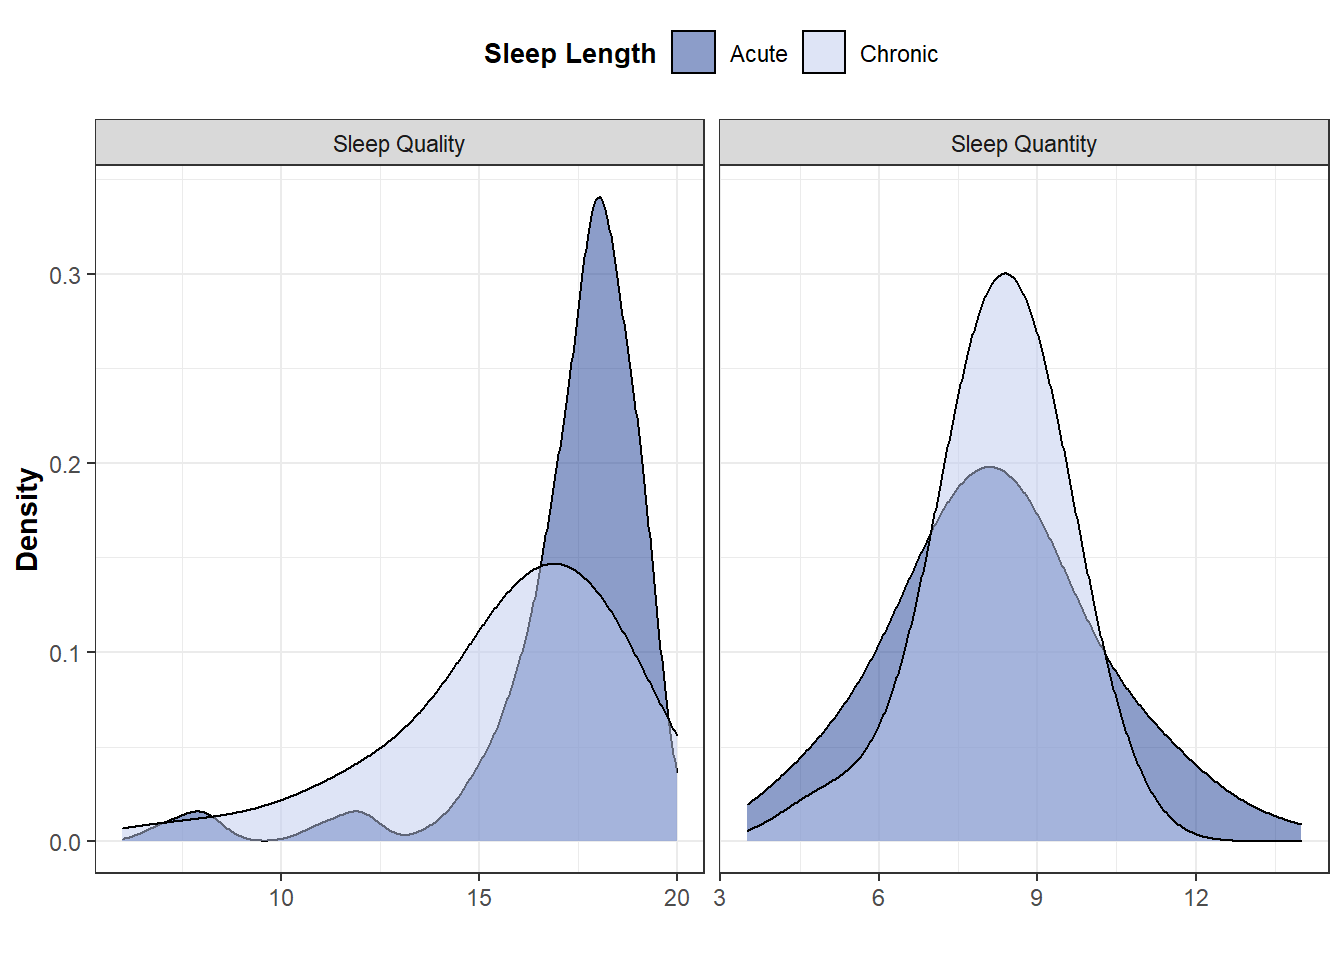
\includegraphics{SupplementaryCode_files/figure-latex/unnamed-chunk-50-1.pdf}

\hypertarget{study-5}{%
\chapter{Study 5}\label{study-5}}

\textbf{Load raw datasets}

\begin{Shaded}
\begin{Highlighting}[]
\NormalTok{Data_Study5_JEPG<-}\KeywordTok{read.delim}\NormalTok{(}\StringTok{"C:/Users/coren/Documents/JEPgeneral/SupplementaryCode/Data/Data-Study5-JEPG.txt"}\NormalTok{)}
\end{Highlighting}
\end{Shaded}

\hypertarget{filter-raw-data-based-upon-inclusion-criteria-missing-data-2}{%
\section{Filter raw data based upon inclusion criteria \& missing data}\label{filter-raw-data-based-upon-inclusion-criteria-missing-data-2}}

\begin{Shaded}
\begin{Highlighting}[]
\NormalTok{Data_Study5_Raw<-}\StringTok{ }\NormalTok{Data_Study5_JEPG }\OperatorTok\StringTok{ }
\StringTok{  }\KeywordTok{mutate}\NormalTok{(}
\CommentTok{#Check for missing Data}
   \DataTypeTok{CCA=}\KeywordTok{case_when}\NormalTok{(}
      \KeywordTok{is.na}\NormalTok{(Moral_DIL) }\OperatorTok{|}\KeywordTok{is.na}\NormalTok{(Moral_SCA) }\OperatorTok{|}\StringTok{ }\KeywordTok{is.na}\NormalTok{(SleepQualCro) }\OperatorTok{|}\StringTok{ }\KeywordTok{is.na}\NormalTok{(SleepQualAcu) }
        \OperatorTok{|}\StringTok{ }\KeywordTok{is.na}\NormalTok{(SleepQuantCro) }\OperatorTok{|}\StringTok{ }\KeywordTok{is.na}\NormalTok{(SleepQuantAcu) }\OperatorTok{~}\DecValTok{0}\NormalTok{, }
      \OperatorTok{!}\KeywordTok{is.na}\NormalTok{(Moral_DIL) }\OperatorTok{&}\StringTok{ }\OperatorTok{!}\KeywordTok{is.na}\NormalTok{(Moral_SCA) }\OperatorTok{&}\StringTok{ }\OperatorTok{!}\KeywordTok{is.na}\NormalTok{(SleepQualCro) }\OperatorTok{&}\StringTok{ }
\StringTok{        }\OperatorTok{!}\KeywordTok{is.na}\NormalTok{(SleepQualAcu) }\OperatorTok{&}\StringTok{ }\OperatorTok{!}\KeywordTok{is.na}\NormalTok{(SleepQuantCro) }\OperatorTok{&}\StringTok{ }\OperatorTok{!}\KeywordTok{is.na}\NormalTok{(SleepQuantAcu) }\OperatorTok{~}\DecValTok{1}\NormalTok{),}
\CommentTok{#Detect age outside targetted range   }
    \DataTypeTok{Age_correct=}\KeywordTok{case_when}\NormalTok{(}
\NormalTok{      Age}\OperatorTok{>=}\DecValTok{18} \OperatorTok{&}\StringTok{ }\NormalTok{Age}\OperatorTok{<=}\DecValTok{50} \OperatorTok{~}\StringTok{ }\DecValTok{1}\NormalTok{,}
\NormalTok{      Age}\OperatorTok{<}\DecValTok{18} \OperatorTok{|}\StringTok{ }\NormalTok{Age}\OperatorTok{>}\DecValTok{50} \OperatorTok{~}\StringTok{ }\DecValTok{0}\NormalTok{))}
\end{Highlighting}
\end{Shaded}

\textbf{Filtering participants not fullfiling these 3 criteria}

\begin{Shaded}
\begin{Highlighting}[]
\NormalTok{Data_Study5_Wide<-}\StringTok{ }\KeywordTok{subset}\NormalTok{(Data_Study5_Raw, Data_Study5_Raw}\OperatorTok{$}\NormalTok{CCA}\OperatorTok{==}\DecValTok{1} \OperatorTok{&}\StringTok{ }\NormalTok{Data_Study5_Raw}\OperatorTok{$}\NormalTok{Age_correct}\OperatorTok{==}\DecValTok{1}\NormalTok{)}
\end{Highlighting}
\end{Shaded}

\hypertarget{data-analysis-4}{%
\section{Data analysis}\label{data-analysis-4}}

\textbf{Run a multivariate regression for each sleep variable (IV) on endorsement of moral principles assessed using moral dilemmas or a moral scale (DVs)}
\#Primary Analysis

\begin{Shaded}
\begin{Highlighting}[]
\NormalTok{QualCroLMS5<-}\KeywordTok{lm}\NormalTok{(}\KeywordTok{cbind}\NormalTok{(Moral_DIL, Moral_SCA)}\OperatorTok{~}\NormalTok{SleepQualCro,Data_Study5_Wide)}
\NormalTok{QualAcuLMS5<-}\KeywordTok{lm}\NormalTok{(}\KeywordTok{cbind}\NormalTok{(Moral_DIL, Moral_SCA)}\OperatorTok{~}\NormalTok{SleepQualAcu,Data_Study5_Wide)}
\NormalTok{QuantCroLMS5<-}\KeywordTok{lm}\NormalTok{(}\KeywordTok{cbind}\NormalTok{(Moral_DIL, Moral_SCA)}\OperatorTok{~}\NormalTok{SleepQuantCro, Data_Study5_Wide)}
\NormalTok{QuantAcuLMS5<-}\KeywordTok{lm}\NormalTok{(}\KeywordTok{cbind}\NormalTok{(Moral_DIL, Moral_SCA)}\OperatorTok{~}\NormalTok{SleepQuantAcu, Data_Study5_Wide)}
\end{Highlighting}
\end{Shaded}

\begin{Shaded}
\begin{Highlighting}[]
\NormalTok{out <-}\StringTok{ }\NormalTok{car}\OperatorTok{:::}\NormalTok{print.Anova.mlm}
\KeywordTok{body}\NormalTok{(out)[[}\DecValTok{16}\NormalTok{]] <-}\StringTok{ }\KeywordTok{quote}\NormalTok{(}\KeywordTok{invisible}\NormalTok{(tests))}
\KeywordTok{body}\NormalTok{(out)[[}\DecValTok{15}\NormalTok{]] <-}\StringTok{ }\OtherTok{NULL}

\CommentTok{#Chronic Sleep Quality}
\NormalTok{FQualCroS5<-}\KeywordTok{round}\NormalTok{(}\KeywordTok{do.call}\NormalTok{(rbind, }\KeywordTok{out}\NormalTok{(}\KeywordTok{Anova}\NormalTok{(QualCroLMS5, }\DataTypeTok{test.statistic=}\StringTok{"Pillai"}\NormalTok{)))[}\DecValTok{3}\NormalTok{], }\DataTypeTok{digit=}\DecValTok{2}\NormalTok{)}
\NormalTok{pQualCroS5<-}\StringTok{  }\KeywordTok{round}\NormalTok{(}\KeywordTok{ifelse}\NormalTok{(}\KeywordTok{do.call}\NormalTok{(rbind, }\KeywordTok{out}\NormalTok{(}\KeywordTok{Anova}\NormalTok{(QualCroLMS5, }\DataTypeTok{test.statistic=}\StringTok{"Pillai"}\NormalTok{)))[}\DecValTok{6}\NormalTok{]}\OperatorTok{*}\DecValTok{4}\OperatorTok{<}\NormalTok{.}\DecValTok{99}\NormalTok{, }\KeywordTok{do.call}\NormalTok{(rbind, }\KeywordTok{out}\NormalTok{(}\KeywordTok{Anova}\NormalTok{(QualCroLMS5, }\DataTypeTok{test.statistic=}\StringTok{"Pillai"}\NormalTok{)))[}\DecValTok{6}\NormalTok{]}\OperatorTok{*}\DecValTok{4}\NormalTok{, }\FloatTok{.99}\NormalTok{), }\DataTypeTok{digit=}\DecValTok{2}\NormalTok{)}

\CommentTok{#Acute Sleep Quality}
\NormalTok{FQualAcuS5<-}\KeywordTok{round}\NormalTok{(}\KeywordTok{do.call}\NormalTok{(rbind, }\KeywordTok{out}\NormalTok{(}\KeywordTok{Anova}\NormalTok{(QualAcuLMS5, }\DataTypeTok{test.statistic=}\StringTok{"Pillai"}\NormalTok{)))[}\DecValTok{3}\NormalTok{], }\DataTypeTok{digit=}\DecValTok{2}\NormalTok{)}
\NormalTok{pQualAcuS5<-}\StringTok{  }\KeywordTok{round}\NormalTok{(}\KeywordTok{ifelse}\NormalTok{(}\KeywordTok{do.call}\NormalTok{(rbind, }\KeywordTok{out}\NormalTok{(}\KeywordTok{Anova}\NormalTok{(QualAcuLMS5, }\DataTypeTok{test.statistic=}\StringTok{"Pillai"}\NormalTok{)))[}\DecValTok{6}\NormalTok{]}\OperatorTok{*}\DecValTok{4}\OperatorTok{<}\NormalTok{.}\DecValTok{99}\NormalTok{, }\KeywordTok{do.call}\NormalTok{(rbind, }\KeywordTok{out}\NormalTok{(}\KeywordTok{Anova}\NormalTok{(QualAcuLMS5, }\DataTypeTok{test.statistic=}\StringTok{"Pillai"}\NormalTok{)))[}\DecValTok{6}\NormalTok{]}\OperatorTok{*}\DecValTok{4}\NormalTok{, }\FloatTok{.99}\NormalTok{), }\DataTypeTok{digit=}\DecValTok{2}\NormalTok{)}

\CommentTok{#Chronic Sleep Quantity}
\NormalTok{FQuantCroS5<-}\KeywordTok{round}\NormalTok{(}\KeywordTok{do.call}\NormalTok{(rbind, }\KeywordTok{out}\NormalTok{(}\KeywordTok{Anova}\NormalTok{(QuantCroLMS5, }\DataTypeTok{test.statistic=}\StringTok{"Pillai"}\NormalTok{)))[}\DecValTok{3}\NormalTok{], }\DataTypeTok{digit=}\DecValTok{2}\NormalTok{)}
\NormalTok{pQuantCroS5<-}\StringTok{  }\KeywordTok{round}\NormalTok{(}\KeywordTok{ifelse}\NormalTok{(}\KeywordTok{do.call}\NormalTok{(rbind, }\KeywordTok{out}\NormalTok{(}\KeywordTok{Anova}\NormalTok{(QuantCroLMS5, }\DataTypeTok{test.statistic=}\StringTok{"Pillai"}\NormalTok{)))[}\DecValTok{6}\NormalTok{]}\OperatorTok{*}\DecValTok{4}\OperatorTok{<}\NormalTok{.}\DecValTok{99}\NormalTok{, }\KeywordTok{do.call}\NormalTok{(rbind, }\KeywordTok{out}\NormalTok{(}\KeywordTok{Anova}\NormalTok{(QuantCroLMS5, }\DataTypeTok{test.statistic=}\StringTok{"Pillai"}\NormalTok{)))[}\DecValTok{6}\NormalTok{]}\OperatorTok{*}\DecValTok{4}\NormalTok{, }\FloatTok{.99}\NormalTok{), }\DataTypeTok{digit=}\DecValTok{2}\NormalTok{)}

\CommentTok{#Acute Sleep Quantity}
\NormalTok{FQuantAcuS5<-}\KeywordTok{round}\NormalTok{(}\KeywordTok{do.call}\NormalTok{(rbind, }\KeywordTok{out}\NormalTok{(}\KeywordTok{Anova}\NormalTok{(QuantCroLMS5, }\DataTypeTok{test.statistic=}\StringTok{"Pillai"}\NormalTok{)))[}\DecValTok{3}\NormalTok{], }\DataTypeTok{digit=}\DecValTok{2}\NormalTok{)}
\NormalTok{pQuantAcuS5<-}\StringTok{  }\KeywordTok{round}\NormalTok{(}\KeywordTok{ifelse}\NormalTok{(}\KeywordTok{do.call}\NormalTok{(rbind, }\KeywordTok{out}\NormalTok{(}\KeywordTok{Anova}\NormalTok{(QuantAcuLMS5, }\DataTypeTok{test.statistic=}\StringTok{"Pillai"}\NormalTok{)))[}\DecValTok{6}\NormalTok{]}\OperatorTok{*}\DecValTok{4}\OperatorTok{<}\NormalTok{.}\DecValTok{99}\NormalTok{, }\KeywordTok{do.call}\NormalTok{(rbind, }\KeywordTok{out}\NormalTok{(}\KeywordTok{Anova}\NormalTok{(QuantAcuLMS5, }\DataTypeTok{test.statistic=}\StringTok{"Pillai"}\NormalTok{)))[}\DecValTok{6}\NormalTok{]}\OperatorTok{*}\DecValTok{4}\NormalTok{, }\FloatTok{.99}\NormalTok{), }\DataTypeTok{digit=}\DecValTok{2}\NormalTok{)}
\end{Highlighting}
\end{Shaded}

\textbf{Put results in a table}

\begin{Shaded}
\begin{Highlighting}[]
\NormalTok{SleepMarker<-}\KeywordTok{c}\NormalTok{(}\StringTok{"Quality Chronic"}\NormalTok{,}\StringTok{"Quality Acute"}\NormalTok{,}\StringTok{"Quantity Chronic"}\NormalTok{,}\StringTok{"Quantity Acute"}\NormalTok{)}
\NormalTok{FS5<-}\KeywordTok{c}\NormalTok{(FQualCroS5,FQualAcuS5,FQuantCroS5,FQuantAcuS5)}
\NormalTok{pvalS5<-}\KeywordTok{c}\NormalTok{(pQualCroS5,pQualAcuS5,pQuantCroS5,pQuantAcuS5)}
\NormalTok{NS5<-}\KeywordTok{c}\NormalTok{(}\KeywordTok{length}\NormalTok{(QualCroLMS5}\OperatorTok{$}\NormalTok{fitted.values)}\OperatorTok{/}\DecValTok{2}\NormalTok{,}
     \KeywordTok{length}\NormalTok{(QualAcuLMS5}\OperatorTok{$}\NormalTok{fitted.values)}\OperatorTok{/}\DecValTok{2}\NormalTok{,}
     \KeywordTok{length}\NormalTok{(QuantCroLMS5}\OperatorTok{$}\NormalTok{fitted.values)}\OperatorTok{/}\DecValTok{2}\NormalTok{,}
     \KeywordTok{length}\NormalTok{(QuantAcuLMS5}\OperatorTok{$}\NormalTok{fitted.values)}\OperatorTok{/}\DecValTok{2}\NormalTok{)}
\NormalTok{ResultsStudy5<-}\KeywordTok{data.frame}\NormalTok{(}\StringTok{"Sleep Indicator"}\NormalTok{=SleepMarker, }\StringTok{"F-test"}\NormalTok{=FS5, }\StringTok{"p values"}\NormalTok{=pvalS5, }\StringTok{"N"}\NormalTok{=NS5)}
\KeywordTok{gt}\NormalTok{(ResultsStudy5)}
\end{Highlighting}
\end{Shaded}

\captionsetup[table]{labelformat=empty,skip=1pt}
\begin{longtable}{crrr}
\toprule
Sleep.Indicator & F.test & p.values & N \\ 
\midrule
Quality Chronic & 0.71 & 0.99 & 105 \\ 
Quality Acute & 0.30 & 0.99 & 105 \\ 
Quantity Chronic & 0.22 & 0.99 & 105 \\ 
Quantity Acute & 0.22 & 0.99 & 105 \\ 
\bottomrule
\end{longtable}

\textbf{Create datasets to display regression summary on the plots}

\begin{Shaded}
\begin{Highlighting}[]
\NormalTok{ResumQualCroS5<-}\StringTok{ }\KeywordTok{paste0}\NormalTok{(}\StringTok{"F="}\NormalTok{,FQualCroS5,}\StringTok{","}\NormalTok{,}\StringTok{"p="}\NormalTok{,pQualCroS5)}
\NormalTok{ResumQualAcuS5<-}\StringTok{ }\KeywordTok{paste0}\NormalTok{(}\StringTok{"F="}\NormalTok{,FQualAcuS5,}\StringTok{","}\NormalTok{, }\StringTok{"p="}\NormalTok{,pQualAcuS5)}
\NormalTok{ResumQuantCroS5<-}\StringTok{ }\KeywordTok{paste0}\NormalTok{(}\StringTok{"F="}\NormalTok{,FQuantCroS5,}\StringTok{","}\NormalTok{,}\StringTok{"p="}\NormalTok{,pQuantCroS5)}
\NormalTok{ResumQuantAcuS5<-}\StringTok{ }\KeywordTok{paste0}\NormalTok{(}\StringTok{"F="}\NormalTok{,FQuantAcuS5,}\StringTok{","}\NormalTok{,}\StringTok{"p="}\NormalTok{,pQuantAcuS5)}

\NormalTok{annotationQualCroS5 <-}\StringTok{ }\KeywordTok{data.frame}\NormalTok{(}\DataTypeTok{x =} \DecValTok{8}\NormalTok{, }\DataTypeTok{y =} \DecValTok{2}\NormalTok{,  }\DataTypeTok{label =}\NormalTok{ ResumQualCroS5)}
\NormalTok{annotationQualAcuS5 <-}\StringTok{ }\KeywordTok{data.frame}\NormalTok{(}\DataTypeTok{x =} \DecValTok{8}\NormalTok{, }\DataTypeTok{y =} \DecValTok{2}\NormalTok{,  }\DataTypeTok{label =}\NormalTok{ ResumQualAcuS5)}
\NormalTok{annotationQuantCroS5 <-}\StringTok{ }\KeywordTok{data.frame}\NormalTok{(}\DataTypeTok{x =}\DecValTok{8}\NormalTok{, }\DataTypeTok{y =} \DecValTok{2}\NormalTok{,  }\DataTypeTok{label =}\NormalTok{ ResumQuantCroS5)}
\NormalTok{annotationQuantAcuS5 <-}\StringTok{ }\KeywordTok{data.frame}\NormalTok{(}\DataTypeTok{x =} \DecValTok{8}\NormalTok{, }\DataTypeTok{y =} \DecValTok{2}\NormalTok{,  }\DataTypeTok{label =}\NormalTok{ ResumQuantAcuS5)}

\NormalTok{annotationS5<-}\KeywordTok{cbind}\NormalTok{(}
  \KeywordTok{rbind}\NormalTok{(annotationQualCroS5, }
\NormalTok{        annotationQualAcuS5, }
\NormalTok{        annotationQuantCroS5, }
\NormalTok{        annotationQuantAcuS5),}
  \DataTypeTok{SleepType=}\KeywordTok{c}\NormalTok{(}
        \StringTok{"Quality of Chronic Sleep"}\NormalTok{, }
        \StringTok{"Quality of Acute Sleep"}\NormalTok{, }
        \StringTok{"Quantity of Chronic Sleep"}\NormalTok{, }
        \StringTok{"Quantity of Acute Sleep"}\NormalTok{))}
\end{Highlighting}
\end{Shaded}

\textbf{Prepare data for plots}

\begin{Shaded}
\begin{Highlighting}[]
\NormalTok{Data_PlotS5<-}\StringTok{ }\NormalTok{Data_Study5_Wide }\OperatorTok
\StringTok{  }\KeywordTok{pivot_longer}\NormalTok{(}
    \DataTypeTok{cols=}\KeywordTok{c}\NormalTok{(SleepQualCro, SleepQualAcu, SleepQuantCro, SleepQuantAcu),}
    \DataTypeTok{names_to=}\StringTok{"SleepType"}\NormalTok{) }\OperatorTok
\StringTok{  }\KeywordTok{rename}\NormalTok{(}\StringTok{"SleepValue"}\NormalTok{=value) }\OperatorTok
\StringTok{  }\KeywordTok{mutate}\NormalTok{(}
    \DataTypeTok{SleepLength=}\KeywordTok{case_when}\NormalTok{(}
\NormalTok{      SleepType}\OperatorTok{==}\StringTok{"SleepQualCro"} \OperatorTok{|}\StringTok{ }\NormalTok{SleepType}\OperatorTok{==}\StringTok{"SleepQuantCro"}\OperatorTok{~}\StringTok{"Chronic"}\NormalTok{,}
\NormalTok{      SleepType}\OperatorTok{==}\StringTok{"SleepQualAcu"} \OperatorTok{|}\StringTok{ }\NormalTok{SleepType}\OperatorTok{==}\StringTok{"SleepQuantAcu"}\OperatorTok{~}\StringTok{"Acute"}\NormalTok{),}
    \DataTypeTok{SleepQuanthist=}\KeywordTok{case_when}\NormalTok{(}
\NormalTok{      SleepType}\OperatorTok{==}\StringTok{"SleepQualCro"} \OperatorTok{|}\StringTok{ }\NormalTok{SleepType}\OperatorTok{==}\StringTok{"SleepQualAcu"}\OperatorTok{~}\StringTok{"Sleep Quality"}\NormalTok{,}
\NormalTok{      SleepType}\OperatorTok{==}\StringTok{"SleepQuantCro"} \OperatorTok{|}\StringTok{ }\NormalTok{SleepType}\OperatorTok{==}\StringTok{"SleepQuantAcu"}\OperatorTok{~}\StringTok{"Sleep Quantity"}\NormalTok{),}
    \DataTypeTok{MoralZ_DIL=}\KeywordTok{scale}\NormalTok{(Moral_DIL, }\DataTypeTok{center =} \OtherTok{TRUE}\NormalTok{, }\DataTypeTok{scale =} \OtherTok{TRUE}\NormalTok{),}
    \DataTypeTok{MoralZ_SCA=}\KeywordTok{scale}\NormalTok{(Moral_SCA, }\DataTypeTok{center =} \OtherTok{TRUE}\NormalTok{, }\DataTypeTok{scale =} \OtherTok{TRUE}\NormalTok{))}

\NormalTok{Data_PlotS5}\OperatorTok{$}\NormalTok{SleepType<-dplyr}\OperatorTok{::}\KeywordTok{recode}\NormalTok{(Data_PlotS5}\OperatorTok{$}\NormalTok{SleepType, }
        \StringTok{"SleepQualCro"}\NormalTok{ =}\StringTok{ "Quality of Chronic Sleep"}\NormalTok{,}
        \StringTok{"SleepQualAcu"}\NormalTok{ =}\StringTok{ "Quality of Acute Sleep"}\NormalTok{,}
        \StringTok{"SleepQuantCro"}\NormalTok{ =}\StringTok{ "Quantity of Chronic Sleep"}\NormalTok{,}
        \StringTok{"SleepQuantAcu"}\NormalTok{ =}\StringTok{ "Quantity of Acute Sleep"}\NormalTok{)}


\NormalTok{Data_ScatterS5<-}\StringTok{ }\NormalTok{Data_PlotS5 }\OperatorTok
\StringTok{  }\KeywordTok{pivot_longer}\NormalTok{(}
    \DataTypeTok{cols=}\KeywordTok{c}\NormalTok{(MoralZ_DIL, MoralZ_SCA),}
    \DataTypeTok{names_to=}\StringTok{"Outcome"}\NormalTok{) }\OperatorTok
\StringTok{  }\KeywordTok{rename}\NormalTok{(}\StringTok{"MoralValue"}\NormalTok{=value)}
\NormalTok{Data_ScatterS5}\OperatorTok{$}\NormalTok{Outcome<-dplyr}\OperatorTok{::}\KeywordTok{recode}\NormalTok{(Data_ScatterS5}\OperatorTok{$}\NormalTok{Outcome, }
        \StringTok{"MoralZ_DIL"}\NormalTok{ =}\StringTok{ "Dilemmas"}\NormalTok{,}
        \StringTok{"MoralZ_SCA"}\NormalTok{ =}\StringTok{ "Scale"}\NormalTok{)}
\end{Highlighting}
\end{Shaded}

\textbf{Plot distribution of each sleep indicator}

\begin{Shaded}
\begin{Highlighting}[]
\NormalTok{DistQualityS5<-}\KeywordTok{ggplot}\NormalTok{(Data_PlotS5, }\KeywordTok{aes}\NormalTok{(}\DataTypeTok{x=}\NormalTok{SleepValue, }\DataTypeTok{fill=}\KeywordTok{factor}\NormalTok{(SleepLength))) }\OperatorTok{+}\StringTok{ }
\StringTok{  }\KeywordTok{geom_density}\NormalTok{(}\DataTypeTok{alpha=}\FloatTok{0.5}\NormalTok{, }\DataTypeTok{size=}\FloatTok{0.5}\NormalTok{,}\DataTypeTok{adjust =} \DecValTok{2}\NormalTok{) }\OperatorTok{+}\StringTok{ }
\StringTok{  }\KeywordTok{scale_fill_manual}\NormalTok{(}\DataTypeTok{values=}\KeywordTok{c}\NormalTok{(}\StringTok{"#193B94"}\NormalTok{, }\StringTok{"#BDCAEE"}\NormalTok{)) }\OperatorTok{+}
\StringTok{  }\KeywordTok{theme_bw}\NormalTok{() }\OperatorTok{+}\StringTok{ }
\StringTok{  }\KeywordTok{ylab}\NormalTok{(}\StringTok{"Density"}\NormalTok{) }\OperatorTok{+}\StringTok{ }\KeywordTok{xlab}\NormalTok{(}\StringTok{""}\NormalTok{) }\OperatorTok{+}
\StringTok{  }\KeywordTok{facet_wrap}\NormalTok{(}\OperatorTok{~}\KeywordTok{factor}\NormalTok{(SleepQuanthist), }\DataTypeTok{scale=}\StringTok{"free_x"}\NormalTok{) }\OperatorTok{+}\StringTok{ }
\StringTok{  }\KeywordTok{guides}\NormalTok{(}\DataTypeTok{fill=}\KeywordTok{guide_legend}\NormalTok{(}\StringTok{"Sleep Length"}\NormalTok{)) }\OperatorTok{+}
\StringTok{  }\KeywordTok{theme}\NormalTok{(}
    \DataTypeTok{axis.title.y =} \KeywordTok{element_text}\NormalTok{(}\DataTypeTok{size =} \DecValTok{11}\NormalTok{, }\DataTypeTok{hjust =} \FloatTok{0.5}\NormalTok{, }\DataTypeTok{face=}\StringTok{"bold"}\NormalTok{),}
    \DataTypeTok{axis.title.x =} \KeywordTok{element_text}\NormalTok{(}\DataTypeTok{face=}\StringTok{"bold"}\NormalTok{, }\DataTypeTok{size =} \DecValTok{11}\NormalTok{, }\DataTypeTok{hjust =} \FloatTok{0.5}\NormalTok{),}
    \DataTypeTok{legend.position=}\StringTok{"top"}\NormalTok{,}
    \DataTypeTok{legend.title =} \KeywordTok{element_text}\NormalTok{(}\DataTypeTok{colour=}\StringTok{"black"}\NormalTok{, }\DataTypeTok{size=}\DecValTok{10}\NormalTok{, }\DataTypeTok{face=}\StringTok{"bold"}\NormalTok{)) }
\NormalTok{DistQualityS5}
\end{Highlighting}
\end{Shaded}

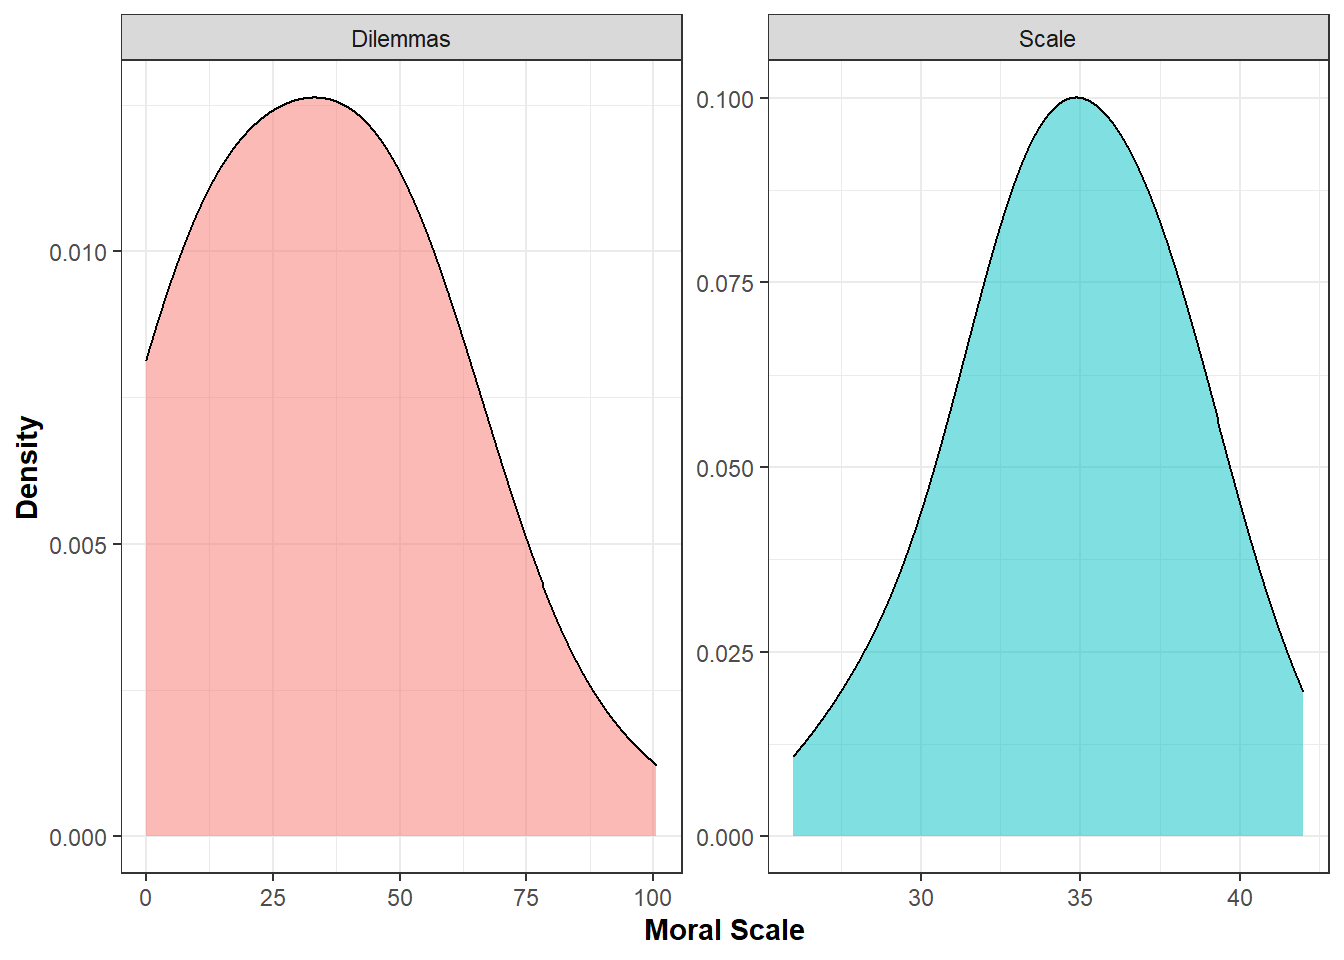
\includegraphics{SupplementaryCode_files/figure-latex/unnamed-chunk-59-1.pdf}

\textbf{N in each sleep quantity category}

\begin{Shaded}
\begin{Highlighting}[]
\NormalTok{Data_Study5_Wide}\OperatorTok{$}\NormalTok{SleepQuantCroR<-}\KeywordTok{round}\NormalTok{(Data_Study5_Wide}\OperatorTok{$}\NormalTok{SleepQuantCro)}
\NormalTok{Data_Study5_Wide}\OperatorTok{$}\NormalTok{SleepQuantAcuR<-}\KeywordTok{round}\NormalTok{(Data_Study5_Wide}\OperatorTok{$}\NormalTok{SleepQuantAcu)}

\NormalTok{Dist.Quantity.ChronicS5<-Data_Study5_Wide }\OperatorTok\StringTok{ }
\StringTok{    }\NormalTok{dplyr}\OperatorTok{::}\KeywordTok{group_by}\NormalTok{(SleepQuantCroR) }\OperatorTok\StringTok{ }
\StringTok{      }\KeywordTok{summarise}\NormalTok{(}
        \DataTypeTok{N=}\KeywordTok{n}\NormalTok{()) }\OperatorTok\StringTok{ }
\StringTok{          }\KeywordTok{spread}\NormalTok{(SleepQuantCroR, N) }\OperatorTok\StringTok{ }
\StringTok{  }\KeywordTok{as.data.frame}\NormalTok{()}
\KeywordTok{row.names}\NormalTok{(Dist.Quantity.ChronicS5)<-}\StringTok{"Quantity Chronic"}

\NormalTok{Dist.Quantity.AcuteS5<-Data_Study5_Wide }\OperatorTok\StringTok{ }
\StringTok{    }\NormalTok{dplyr}\OperatorTok{::}\KeywordTok{group_by}\NormalTok{(SleepQuantAcuR) }\OperatorTok\StringTok{ }
\StringTok{      }\KeywordTok{summarise}\NormalTok{(}
        \DataTypeTok{N=}\KeywordTok{n}\NormalTok{()) }\OperatorTok\StringTok{ }
\StringTok{          }\KeywordTok{spread}\NormalTok{(SleepQuantAcuR, N) }\OperatorTok\StringTok{ }
\StringTok{  }\KeywordTok{as.data.frame}\NormalTok{()}
\KeywordTok{row.names}\NormalTok{(Dist.Quantity.AcuteS5)<-}\StringTok{"Quantity Acute"}

\KeywordTok{bind_rows}\NormalTok{(Dist.Quantity.AcuteS5, Dist.Quantity.ChronicS5)}
\end{Highlighting}
\end{Shaded}

\begin{verbatim}
##                  4 5 6  7  8  9 10 11 12 13 14
## Quantity Acute   3 6 7 20 28 19  7  8  5  1  1
## Quantity Chronic 1 4 5 13 36 31 12  3 NA NA NA
\end{verbatim}

\textbf{Scatterplots}

\begin{Shaded}
\begin{Highlighting}[]
\KeywordTok{ggplot}\NormalTok{(Data_ScatterS5, }\KeywordTok{aes}\NormalTok{(}\DataTypeTok{x=}\NormalTok{SleepValue, }\DataTypeTok{y=}\NormalTok{MoralValue, }\DataTypeTok{color=}\NormalTok{Outcome, }\DataTypeTok{fill=}\NormalTok{Outcome)) }\OperatorTok{+}\StringTok{ }
\StringTok{       }\KeywordTok{geom_smooth}\NormalTok{(}\DataTypeTok{method=}\StringTok{"lm"}\NormalTok{ )}\OperatorTok{+}
\StringTok{      }\KeywordTok{geom_point}\NormalTok{(}\DataTypeTok{alpha=}\FloatTok{0.2}\NormalTok{)}\OperatorTok{+}
\StringTok{       }\KeywordTok{facet_wrap}\NormalTok{(}\OperatorTok{~}\KeywordTok{factor}\NormalTok{(SleepType), }\DataTypeTok{scales=}\StringTok{"free_x"}\NormalTok{) }\OperatorTok{+}
\StringTok{       }\KeywordTok{theme_bw}\NormalTok{() }\OperatorTok{+}\StringTok{ }\KeywordTok{ylab}\NormalTok{(}\StringTok{"Utilitirianism"}\NormalTok{) }\OperatorTok{+}\StringTok{ }\KeywordTok{xlab}\NormalTok{(}\StringTok{""}\NormalTok{) }\OperatorTok{+}\StringTok{ }
\StringTok{       }\KeywordTok{theme}\NormalTok{(}\DataTypeTok{axis.title.y =} \KeywordTok{element_text}\NormalTok{(}\DataTypeTok{size =} \DecValTok{11}\NormalTok{, }\DataTypeTok{hjust =} \FloatTok{0.5}\NormalTok{, }\DataTypeTok{face=}\StringTok{"bold"}\NormalTok{), }
             \DataTypeTok{axis.title.x =} \KeywordTok{element_text}\NormalTok{(}\DataTypeTok{face=}\StringTok{"bold"}\NormalTok{, }\DataTypeTok{size =} \DecValTok{11}\NormalTok{, }\DataTypeTok{hjust =} \FloatTok{0.5}\NormalTok{)) }\OperatorTok{+}
\StringTok{       }\KeywordTok{guides}\NormalTok{(}\DataTypeTok{size=}\OtherTok{FALSE}\NormalTok{, }\DataTypeTok{colour=}\OtherTok{FALSE}\NormalTok{) }\OperatorTok{+}\StringTok{ }
\StringTok{       }\KeywordTok{scale_fill_manual}\NormalTok{(}\DataTypeTok{values=}\KeywordTok{c}\NormalTok{(}\StringTok{"red"}\NormalTok{,}\StringTok{"#193B94"}\NormalTok{))}\OperatorTok{+}
\StringTok{       }\KeywordTok{scale_color_manual}\NormalTok{(}\DataTypeTok{values=}\KeywordTok{c}\NormalTok{(}\StringTok{"red"}\NormalTok{,}\StringTok{"#193B94"}\NormalTok{))}\OperatorTok{+}

\StringTok{       }\KeywordTok{geom_label}\NormalTok{(}\DataTypeTok{data=}\NormalTok{annotationS5, }\KeywordTok{aes}\NormalTok{( }\DataTypeTok{x=}\NormalTok{x, }\DataTypeTok{y=}\NormalTok{y, }\DataTypeTok{label=}\NormalTok{label), }
                  \DataTypeTok{color=}\StringTok{"black"}\NormalTok{,  }\DataTypeTok{size=}\FloatTok{3.5}\NormalTok{ , }\DataTypeTok{angle=}\DecValTok{45}\NormalTok{, }\DataTypeTok{alpha=}\DecValTok{7}\OperatorTok{/}\DecValTok{10}\NormalTok{, }\DataTypeTok{inherit.aes =} \OtherTok{FALSE}\NormalTok{)}
\end{Highlighting}
\end{Shaded}

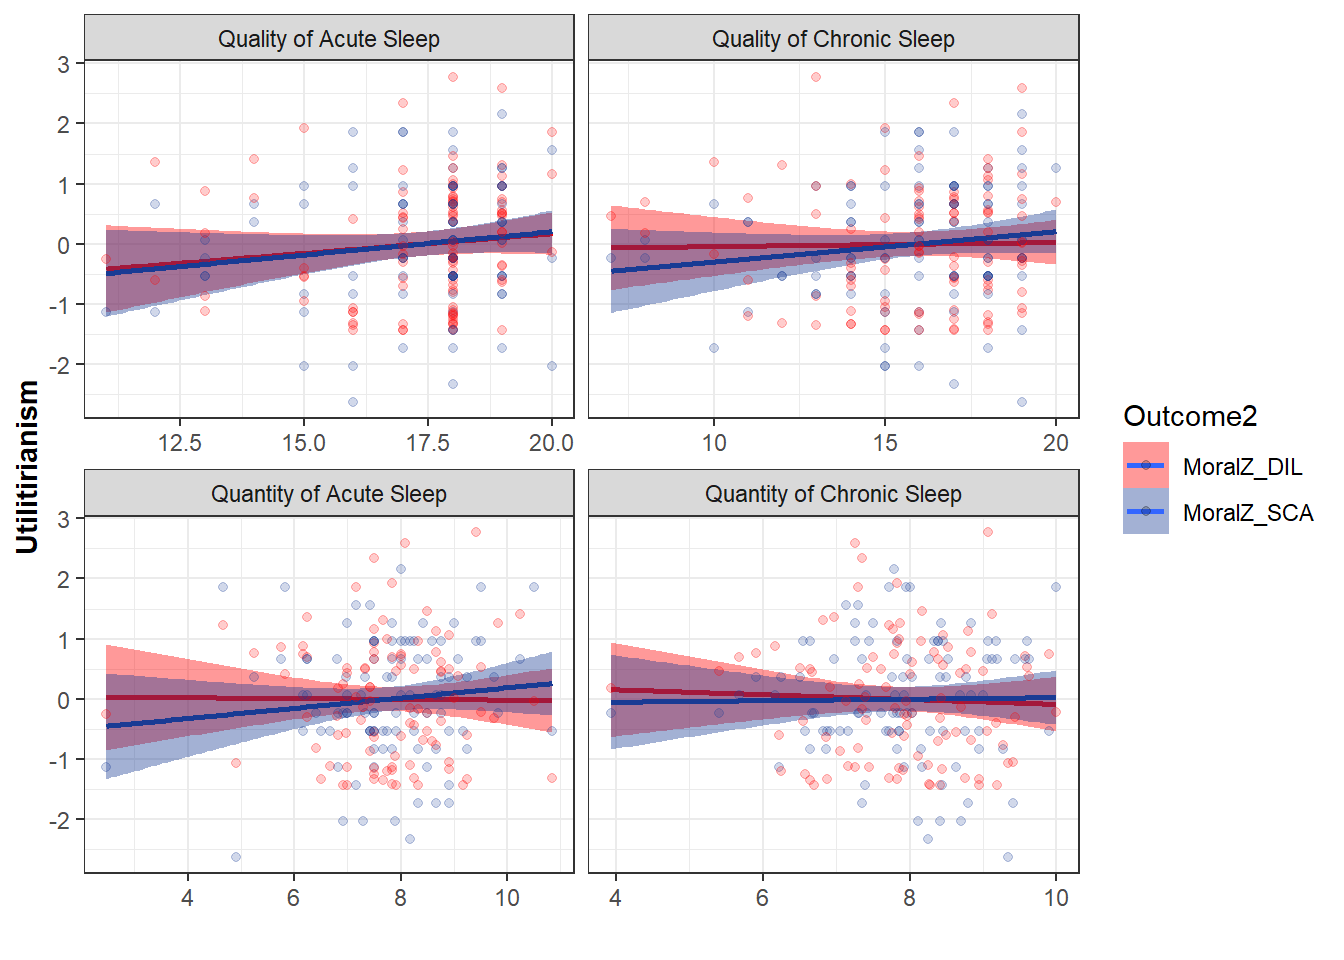
\includegraphics{SupplementaryCode_files/figure-latex/unnamed-chunk-61-1.pdf}

\hypertarget{study-6}{%
\chapter{Study 6}\label{study-6}}

\textbf{Load raw datasets}

\begin{Shaded}
\begin{Highlighting}[]
\NormalTok{Data_Study6_JEPG<-}\KeywordTok{read.delim}\NormalTok{(}\StringTok{"C:/Users/coren/Documents/JEPgeneral/SupplementaryCode/Data/Data-Study6-JEPG.txt"}\NormalTok{)}
\end{Highlighting}
\end{Shaded}

\hypertarget{filter-raw-data-based-upon-inclusion-criteria-missing-data-3}{%
\section{Filter raw data based upon inclusion criteria \& missing data}\label{filter-raw-data-based-upon-inclusion-criteria-missing-data-3}}

\begin{Shaded}
\begin{Highlighting}[]
\NormalTok{Data_Study6_Raw<-}\StringTok{ }\NormalTok{Data_Study6_JEPG }\OperatorTok\StringTok{ }
\StringTok{  }\KeywordTok{mutate}\NormalTok{(}
\CommentTok{#Check for missing Data}
   \DataTypeTok{CCA=}\KeywordTok{case_when}\NormalTok{(}
      \KeywordTok{is.na}\NormalTok{(Moral_DIL) }\OperatorTok{|}\KeywordTok{is.na}\NormalTok{(Moral_SCA) }\OperatorTok{|}\StringTok{ }\KeywordTok{is.na}\NormalTok{(SleepQualCro) }\OperatorTok{|}\StringTok{ }\KeywordTok{is.na}\NormalTok{(SleepQualAcu) }
        \OperatorTok{|}\StringTok{ }\KeywordTok{is.na}\NormalTok{(SleepQuantCro) }\OperatorTok{|}\StringTok{ }\KeywordTok{is.na}\NormalTok{(SleepQuantAcu) }\OperatorTok{~}\DecValTok{0}\NormalTok{, }
      \OperatorTok{!}\KeywordTok{is.na}\NormalTok{(Moral_DIL) }\OperatorTok{&}\StringTok{ }\OperatorTok{!}\KeywordTok{is.na}\NormalTok{(Moral_SCA) }\OperatorTok{&}\StringTok{ }\OperatorTok{!}\KeywordTok{is.na}\NormalTok{(SleepQualCro) }\OperatorTok{&}\StringTok{ }
\StringTok{        }\OperatorTok{!}\KeywordTok{is.na}\NormalTok{(SleepQualAcu) }\OperatorTok{&}\StringTok{ }\OperatorTok{!}\KeywordTok{is.na}\NormalTok{(SleepQuantCro) }\OperatorTok{&}\StringTok{ }\OperatorTok{!}\KeywordTok{is.na}\NormalTok{(SleepQuantAcu) }\OperatorTok{~}\DecValTok{1}\NormalTok{),}
\CommentTok{#Detect age outside targetted range   }
    \DataTypeTok{Age_correct=}\KeywordTok{case_when}\NormalTok{(}
\NormalTok{      Age}\OperatorTok{>=}\DecValTok{18} \OperatorTok{&}\StringTok{ }\NormalTok{Age}\OperatorTok{<=}\DecValTok{50} \OperatorTok{~}\StringTok{ }\DecValTok{1}\NormalTok{,}
\NormalTok{      Age}\OperatorTok{<}\DecValTok{18} \OperatorTok{|}\StringTok{ }\NormalTok{Age}\OperatorTok{>}\DecValTok{50} \OperatorTok{~}\StringTok{ }\DecValTok{0}\NormalTok{),}
    \DataTypeTok{Attention_check=}\KeywordTok{case_when}\NormalTok{(}
\NormalTok{      Tromp}\OperatorTok{==}\DecValTok{1}\OperatorTok{~}\DecValTok{1}\NormalTok{,}
\NormalTok{      Tromp}\OperatorTok{!=}\DecValTok{1}\OperatorTok{~}\DecValTok{0}
\NormalTok{    ))}
\end{Highlighting}
\end{Shaded}

\textbf{Filtering participants not fullfiling these 3 criteria}

\begin{Shaded}
\begin{Highlighting}[]
\NormalTok{Data_Study6_Wide<-}\StringTok{ }\KeywordTok{subset}\NormalTok{(Data_Study6_Raw, Data_Study6_Raw}\OperatorTok{$}\NormalTok{CCA}\OperatorTok{==}\DecValTok{1} \OperatorTok{&}\StringTok{ }\NormalTok{Data_Study6_Raw}\OperatorTok{$}\NormalTok{Age_correct}\OperatorTok{==}\DecValTok{1} \OperatorTok{&}\StringTok{ }\NormalTok{Data_Study6_Raw}\OperatorTok{$}\NormalTok{Attention_check}\OperatorTok{==}\DecValTok{1}\NormalTok{)}
\end{Highlighting}
\end{Shaded}

\hypertarget{data-analysis-5}{%
\section{Data analysis}\label{data-analysis-5}}

\textbf{Run a multivariate regression for each sleep variable (IV) on endorsement of moral principles assessed using moral dilemmas or a moral scale (DVs)}
\#Primary Analysis

\begin{Shaded}
\begin{Highlighting}[]
\NormalTok{QualCroLMS6<-}\KeywordTok{lm}\NormalTok{(}\KeywordTok{cbind}\NormalTok{(Moral_DIL, Moral_SCA)}\OperatorTok{~}\NormalTok{SleepQualCro,Data_Study6_Wide)}
\NormalTok{QualAcuLMS6<-}\KeywordTok{lm}\NormalTok{(}\KeywordTok{cbind}\NormalTok{(Moral_DIL, Moral_SCA)}\OperatorTok{~}\NormalTok{SleepQualAcu,Data_Study6_Wide)}
\NormalTok{QuantCroLMS6<-}\KeywordTok{lm}\NormalTok{(}\KeywordTok{cbind}\NormalTok{(Moral_DIL, Moral_SCA)}\OperatorTok{~}\NormalTok{SleepQuantCro, Data_Study6_Wide)}
\NormalTok{QuantAcuLMS6<-}\KeywordTok{lm}\NormalTok{(}\KeywordTok{cbind}\NormalTok{(Moral_DIL, Moral_SCA)}\OperatorTok{~}\NormalTok{SleepQuantAcu, Data_Study6_Wide)}
\end{Highlighting}
\end{Shaded}

\begin{Shaded}
\begin{Highlighting}[]
\NormalTok{out <-}\StringTok{ }\NormalTok{car}\OperatorTok{:::}\NormalTok{print.Anova.mlm}
\KeywordTok{body}\NormalTok{(out)[[}\DecValTok{16}\NormalTok{]] <-}\StringTok{ }\KeywordTok{quote}\NormalTok{(}\KeywordTok{invisible}\NormalTok{(tests))}
\KeywordTok{body}\NormalTok{(out)[[}\DecValTok{15}\NormalTok{]] <-}\StringTok{ }\OtherTok{NULL}

\CommentTok{#Chronic Sleep Quality}
\NormalTok{FQualCroS6<-}\KeywordTok{round}\NormalTok{(}\KeywordTok{do.call}\NormalTok{(rbind, }\KeywordTok{out}\NormalTok{(}\KeywordTok{Anova}\NormalTok{(QualCroLMS6, }\DataTypeTok{test.statistic=}\StringTok{"Pillai"}\NormalTok{)))[}\DecValTok{3}\NormalTok{], }\DataTypeTok{digit=}\DecValTok{2}\NormalTok{)}
\NormalTok{pQualCroS6<-}\StringTok{  }\KeywordTok{round}\NormalTok{(}\KeywordTok{ifelse}\NormalTok{(}\KeywordTok{do.call}\NormalTok{(rbind, }\KeywordTok{out}\NormalTok{(}\KeywordTok{Anova}\NormalTok{(QualCroLMS6, }\DataTypeTok{test.statistic=}\StringTok{"Pillai"}\NormalTok{)))[}\DecValTok{6}\NormalTok{]}\OperatorTok{*}\DecValTok{4}\OperatorTok{<}\NormalTok{.}\DecValTok{99}\NormalTok{, }\KeywordTok{do.call}\NormalTok{(rbind, }\KeywordTok{out}\NormalTok{(}\KeywordTok{Anova}\NormalTok{(QualCroLMS6, }\DataTypeTok{test.statistic=}\StringTok{"Pillai"}\NormalTok{)))[}\DecValTok{6}\NormalTok{]}\OperatorTok{*}\DecValTok{4}\NormalTok{, }\FloatTok{.99}\NormalTok{), }\DataTypeTok{digit=}\DecValTok{2}\NormalTok{)}

\CommentTok{#Acute Sleep Quality}
\NormalTok{FQualAcuS6<-}\KeywordTok{round}\NormalTok{(}\KeywordTok{do.call}\NormalTok{(rbind, }\KeywordTok{out}\NormalTok{(}\KeywordTok{Anova}\NormalTok{(QualAcuLMS6, }\DataTypeTok{test.statistic=}\StringTok{"Pillai"}\NormalTok{)))[}\DecValTok{3}\NormalTok{], }\DataTypeTok{digit=}\DecValTok{2}\NormalTok{)}
\NormalTok{pQualAcuS6<-}\StringTok{  }\KeywordTok{round}\NormalTok{(}\KeywordTok{ifelse}\NormalTok{(}\KeywordTok{do.call}\NormalTok{(rbind, }\KeywordTok{out}\NormalTok{(}\KeywordTok{Anova}\NormalTok{(QualAcuLMS6, }\DataTypeTok{test.statistic=}\StringTok{"Pillai"}\NormalTok{)))[}\DecValTok{6}\NormalTok{]}\OperatorTok{*}\DecValTok{4}\OperatorTok{<}\NormalTok{.}\DecValTok{99}\NormalTok{, }\KeywordTok{do.call}\NormalTok{(rbind, }\KeywordTok{out}\NormalTok{(}\KeywordTok{Anova}\NormalTok{(QualAcuLMS6, }\DataTypeTok{test.statistic=}\StringTok{"Pillai"}\NormalTok{)))[}\DecValTok{6}\NormalTok{]}\OperatorTok{*}\DecValTok{4}\NormalTok{, }\FloatTok{.99}\NormalTok{), }\DataTypeTok{digit=}\DecValTok{2}\NormalTok{)}

\CommentTok{#Chronic Sleep Quantity}
\NormalTok{FQuantCroS6<-}\KeywordTok{round}\NormalTok{(}\KeywordTok{do.call}\NormalTok{(rbind, }\KeywordTok{out}\NormalTok{(}\KeywordTok{Anova}\NormalTok{(QuantCroLMS6, }\DataTypeTok{test.statistic=}\StringTok{"Pillai"}\NormalTok{)))[}\DecValTok{3}\NormalTok{], }\DataTypeTok{digit=}\DecValTok{2}\NormalTok{)}
\NormalTok{pQuantCroS6<-}\StringTok{  }\KeywordTok{round}\NormalTok{(}\KeywordTok{ifelse}\NormalTok{(}\KeywordTok{do.call}\NormalTok{(rbind, }\KeywordTok{out}\NormalTok{(}\KeywordTok{Anova}\NormalTok{(QuantCroLMS6, }\DataTypeTok{test.statistic=}\StringTok{"Pillai"}\NormalTok{)))[}\DecValTok{6}\NormalTok{]}\OperatorTok{*}\DecValTok{4}\OperatorTok{<}\NormalTok{.}\DecValTok{99}\NormalTok{, }\KeywordTok{do.call}\NormalTok{(rbind, }\KeywordTok{out}\NormalTok{(}\KeywordTok{Anova}\NormalTok{(QuantCroLMS6, }\DataTypeTok{test.statistic=}\StringTok{"Pillai"}\NormalTok{)))[}\DecValTok{6}\NormalTok{]}\OperatorTok{*}\DecValTok{4}\NormalTok{, }\FloatTok{.99}\NormalTok{), }\DataTypeTok{digit=}\DecValTok{2}\NormalTok{)}

\CommentTok{#Acute Sleep Quantity}
\NormalTok{FQuantAcuS6<-}\KeywordTok{round}\NormalTok{(}\KeywordTok{do.call}\NormalTok{(rbind, }\KeywordTok{out}\NormalTok{(}\KeywordTok{Anova}\NormalTok{(QuantCroLMS6, }\DataTypeTok{test.statistic=}\StringTok{"Pillai"}\NormalTok{)))[}\DecValTok{3}\NormalTok{], }\DataTypeTok{digit=}\DecValTok{2}\NormalTok{)}
\NormalTok{pQuantAcuS6<-}\StringTok{  }\KeywordTok{round}\NormalTok{(}\KeywordTok{ifelse}\NormalTok{(}\KeywordTok{do.call}\NormalTok{(rbind, }\KeywordTok{out}\NormalTok{(}\KeywordTok{Anova}\NormalTok{(QuantAcuLMS6, }\DataTypeTok{test.statistic=}\StringTok{"Pillai"}\NormalTok{)))[}\DecValTok{6}\NormalTok{]}\OperatorTok{*}\DecValTok{4}\OperatorTok{<}\NormalTok{.}\DecValTok{99}\NormalTok{, }\KeywordTok{do.call}\NormalTok{(rbind, }\KeywordTok{out}\NormalTok{(}\KeywordTok{Anova}\NormalTok{(QuantAcuLMS6, }\DataTypeTok{test.statistic=}\StringTok{"Pillai"}\NormalTok{)))[}\DecValTok{6}\NormalTok{]}\OperatorTok{*}\DecValTok{4}\NormalTok{, }\FloatTok{.99}\NormalTok{), }\DataTypeTok{digit=}\DecValTok{2}\NormalTok{)}
\end{Highlighting}
\end{Shaded}

\textbf{Put results in a table}

\begin{Shaded}
\begin{Highlighting}[]
\NormalTok{SleepMarker<-}\KeywordTok{c}\NormalTok{(}\StringTok{"Quality Chronic"}\NormalTok{,}\StringTok{"Quality Acute"}\NormalTok{,}\StringTok{"Quantity Chronic"}\NormalTok{,}\StringTok{"Quantity Acute"}\NormalTok{)}
\NormalTok{FS6<-}\KeywordTok{c}\NormalTok{(FQualCroS6,FQualAcuS6,FQuantCroS6,FQuantAcuS6)}
\NormalTok{pvalS6<-}\KeywordTok{c}\NormalTok{(pQualCroS6,pQualAcuS6,pQuantCroS6,pQuantAcuS6)}
\NormalTok{NS6<-}\KeywordTok{c}\NormalTok{(}\KeywordTok{length}\NormalTok{(QualCroLMS6}\OperatorTok{$}\NormalTok{fitted.values)}\OperatorTok{/}\DecValTok{2}\NormalTok{,}
     \KeywordTok{length}\NormalTok{(QualAcuLMS6}\OperatorTok{$}\NormalTok{fitted.values)}\OperatorTok{/}\DecValTok{2}\NormalTok{,}
     \KeywordTok{length}\NormalTok{(QuantCroLMS6}\OperatorTok{$}\NormalTok{fitted.values)}\OperatorTok{/}\DecValTok{2}\NormalTok{,}
     \KeywordTok{length}\NormalTok{(QuantAcuLMS6}\OperatorTok{$}\NormalTok{fitted.values)}\OperatorTok{/}\DecValTok{2}\NormalTok{)}
\NormalTok{ResultsStudy6<-}\KeywordTok{data.frame}\NormalTok{(}\StringTok{"Sleep Indicator"}\NormalTok{=SleepMarker, }\StringTok{"F-test"}\NormalTok{=FS6, }\StringTok{"p values"}\NormalTok{=pvalS6, }\StringTok{"N"}\NormalTok{=NS6)}
\KeywordTok{gt}\NormalTok{(ResultsStudy6)}
\end{Highlighting}
\end{Shaded}

\captionsetup[table]{labelformat=empty,skip=1pt}
\begin{longtable}{crrr}
\toprule
Sleep.Indicator & F.test & p.values & N \\ 
\midrule
Quality Chronic & 0.91 & 0.99 & 99 \\ 
Quality Acute & 1.19 & 0.99 & 99 \\ 
Quantity Chronic & 0.12 & 0.99 & 99 \\ 
Quantity Acute & 0.12 & 0.99 & 99 \\ 
\bottomrule
\end{longtable}

\textbf{Create datasets to display regression summary on the plots}

\begin{Shaded}
\begin{Highlighting}[]
\NormalTok{ResumQualCroS6<-}\StringTok{ }\KeywordTok{paste0}\NormalTok{(}\StringTok{"F="}\NormalTok{,FQualCroS6,}\StringTok{","}\NormalTok{,}\StringTok{"p="}\NormalTok{,pQualCroS6)}
\NormalTok{ResumQualAcuS6<-}\StringTok{ }\KeywordTok{paste0}\NormalTok{(}\StringTok{"F="}\NormalTok{,FQualAcuS6,}\StringTok{","}\NormalTok{, }\StringTok{"p="}\NormalTok{,pQualAcuS6)}
\NormalTok{ResumQuantCroS6<-}\StringTok{ }\KeywordTok{paste0}\NormalTok{(}\StringTok{"F="}\NormalTok{,FQuantCroS6,}\StringTok{","}\NormalTok{,}\StringTok{"p="}\NormalTok{,pQuantCroS6)}
\NormalTok{ResumQuantAcuS6<-}\StringTok{ }\KeywordTok{paste0}\NormalTok{(}\StringTok{"F="}\NormalTok{,FQuantAcuS6,}\StringTok{","}\NormalTok{,}\StringTok{"p="}\NormalTok{,pQuantAcuS6)}

\NormalTok{annotationQualCroS6 <-}\StringTok{ }\KeywordTok{data.frame}\NormalTok{(}\DataTypeTok{x =} \FloatTok{6.5}\NormalTok{, }\DataTypeTok{y =} \FloatTok{2.5}\NormalTok{,  }\DataTypeTok{label =}\NormalTok{ ResumQualCroS6)}
\NormalTok{annotationQualAcuS6 <-}\StringTok{ }\KeywordTok{data.frame}\NormalTok{(}\DataTypeTok{x =} \FloatTok{6.5}\NormalTok{, }\DataTypeTok{y =} \FloatTok{2.5}\NormalTok{,  }\DataTypeTok{label =}\NormalTok{ ResumQualAcuS6)}
\NormalTok{annotationQuantCroS6 <-}\StringTok{ }\KeywordTok{data.frame}\NormalTok{(}\DataTypeTok{x =}\DecValTok{7}\NormalTok{, }\DataTypeTok{y =} \FloatTok{2.5}\NormalTok{,  }\DataTypeTok{label =}\NormalTok{ ResumQuantCroS6)}
\NormalTok{annotationQuantAcuS6 <-}\StringTok{ }\KeywordTok{data.frame}\NormalTok{(}\DataTypeTok{x =} \DecValTok{7}\NormalTok{, }\DataTypeTok{y =} \FloatTok{2.5}\NormalTok{,  }\DataTypeTok{label =}\NormalTok{ ResumQuantAcuS6)}

\NormalTok{annotationS6<-}\KeywordTok{cbind}\NormalTok{(}
  \KeywordTok{rbind}\NormalTok{(annotationQualCroS6, }
\NormalTok{        annotationQualAcuS6, }
\NormalTok{        annotationQuantCroS6, }
\NormalTok{        annotationQuantAcuS6),}
  \DataTypeTok{SleepType=}\KeywordTok{c}\NormalTok{(}
        \StringTok{"Quality of Chronic Sleep"}\NormalTok{, }
        \StringTok{"Quality of Acute Sleep"}\NormalTok{, }
        \StringTok{"Quantity of Chronic Sleep"}\NormalTok{, }
        \StringTok{"Quantity of Acute Sleep"}\NormalTok{))}
\end{Highlighting}
\end{Shaded}

\textbf{Prepare data for plots}

\begin{Shaded}
\begin{Highlighting}[]
\NormalTok{Data_PlotS6<-}\StringTok{ }\NormalTok{Data_Study6_Wide }\OperatorTok
\StringTok{  }\KeywordTok{pivot_longer}\NormalTok{(}
    \DataTypeTok{cols=}\KeywordTok{c}\NormalTok{(SleepQualCro, SleepQualAcu, SleepQuantCro, SleepQuantAcu),}
    \DataTypeTok{names_to=}\StringTok{"SleepType"}\NormalTok{) }\OperatorTok
\StringTok{  }\KeywordTok{rename}\NormalTok{(}\StringTok{"SleepValue"}\NormalTok{=value) }\OperatorTok
\StringTok{  }\KeywordTok{mutate}\NormalTok{(}
    \DataTypeTok{SleepLength=}\KeywordTok{case_when}\NormalTok{(}
\NormalTok{      SleepType}\OperatorTok{==}\StringTok{"SleepQualCro"} \OperatorTok{|}\StringTok{ }\NormalTok{SleepType}\OperatorTok{==}\StringTok{"SleepQuantCro"}\OperatorTok{~}\StringTok{"Chronic"}\NormalTok{,}
\NormalTok{      SleepType}\OperatorTok{==}\StringTok{"SleepQualAcu"} \OperatorTok{|}\StringTok{ }\NormalTok{SleepType}\OperatorTok{==}\StringTok{"SleepQuantAcu"}\OperatorTok{~}\StringTok{"Acute"}\NormalTok{),}
    \DataTypeTok{SleepQuanthist=}\KeywordTok{case_when}\NormalTok{(}
\NormalTok{      SleepType}\OperatorTok{==}\StringTok{"SleepQualCro"} \OperatorTok{|}\StringTok{ }\NormalTok{SleepType}\OperatorTok{==}\StringTok{"SleepQualAcu"}\OperatorTok{~}\StringTok{"Sleep Quality"}\NormalTok{,}
\NormalTok{      SleepType}\OperatorTok{==}\StringTok{"SleepQuantCro"} \OperatorTok{|}\StringTok{ }\NormalTok{SleepType}\OperatorTok{==}\StringTok{"SleepQuantAcu"}\OperatorTok{~}\StringTok{"Sleep Quantity"}\NormalTok{),}
    \DataTypeTok{MoralZ_DIL=}\KeywordTok{scale}\NormalTok{(Moral_DIL, }\DataTypeTok{center =} \OtherTok{TRUE}\NormalTok{, }\DataTypeTok{scale =} \OtherTok{TRUE}\NormalTok{),}
    \DataTypeTok{MoralZ_SCA=}\KeywordTok{scale}\NormalTok{(Moral_SCA, }\DataTypeTok{center =} \OtherTok{TRUE}\NormalTok{, }\DataTypeTok{scale =} \OtherTok{TRUE}\NormalTok{))}

\NormalTok{Data_PlotS6}\OperatorTok{$}\NormalTok{SleepType<-dplyr}\OperatorTok{::}\KeywordTok{recode}\NormalTok{(Data_PlotS6}\OperatorTok{$}\NormalTok{SleepType, }
        \StringTok{"SleepQualCro"}\NormalTok{ =}\StringTok{ "Quality of Chronic Sleep"}\NormalTok{,}
        \StringTok{"SleepQualAcu"}\NormalTok{ =}\StringTok{ "Quality of Acute Sleep"}\NormalTok{,}
        \StringTok{"SleepQuantCro"}\NormalTok{ =}\StringTok{ "Quantity of Chronic Sleep"}\NormalTok{,}
        \StringTok{"SleepQuantAcu"}\NormalTok{ =}\StringTok{ "Quantity of Acute Sleep"}\NormalTok{)}


\NormalTok{Data_ScatterS6<-}\StringTok{ }\NormalTok{Data_PlotS6 }\OperatorTok
\StringTok{  }\KeywordTok{pivot_longer}\NormalTok{(}
    \DataTypeTok{cols=}\KeywordTok{c}\NormalTok{(MoralZ_DIL, MoralZ_SCA),}
    \DataTypeTok{names_to=}\StringTok{"Outcome"}\NormalTok{) }\OperatorTok
\StringTok{  }\KeywordTok{rename}\NormalTok{(}\StringTok{"MoralValue"}\NormalTok{=value)}
\NormalTok{Data_ScatterS6}\OperatorTok{$}\NormalTok{Outcome<-dplyr}\OperatorTok{::}\KeywordTok{recode}\NormalTok{(Data_ScatterS6}\OperatorTok{$}\NormalTok{Outcome, }
        \StringTok{"MoralZ_DIL"}\NormalTok{ =}\StringTok{ "Dilemmas"}\NormalTok{,}
        \StringTok{"MoralZ_SCA"}\NormalTok{ =}\StringTok{ "Scale"}\NormalTok{)}
\end{Highlighting}
\end{Shaded}

\textbf{Plot distribution of each sleep indicator}

\begin{Shaded}
\begin{Highlighting}[]
\NormalTok{DistQualityS6<-}\KeywordTok{ggplot}\NormalTok{(Data_PlotS6, }\KeywordTok{aes}\NormalTok{(}\DataTypeTok{x=}\NormalTok{SleepValue, }\DataTypeTok{fill=}\KeywordTok{factor}\NormalTok{(SleepLength))) }\OperatorTok{+}\StringTok{ }
\StringTok{  }\KeywordTok{geom_density}\NormalTok{(}\DataTypeTok{alpha=}\FloatTok{0.5}\NormalTok{, }\DataTypeTok{size=}\FloatTok{0.5}\NormalTok{,}\DataTypeTok{adjust =} \DecValTok{2}\NormalTok{) }\OperatorTok{+}\StringTok{ }
\StringTok{  }\KeywordTok{scale_fill_manual}\NormalTok{(}\DataTypeTok{values=}\KeywordTok{c}\NormalTok{(}\StringTok{"#193B94"}\NormalTok{, }\StringTok{"#BDCAEE"}\NormalTok{)) }\OperatorTok{+}
\StringTok{  }\KeywordTok{theme_bw}\NormalTok{() }\OperatorTok{+}\StringTok{ }
\StringTok{  }\KeywordTok{ylab}\NormalTok{(}\StringTok{"Density"}\NormalTok{) }\OperatorTok{+}\StringTok{ }\KeywordTok{xlab}\NormalTok{(}\StringTok{""}\NormalTok{) }\OperatorTok{+}
\StringTok{  }\KeywordTok{facet_wrap}\NormalTok{(}\OperatorTok{~}\KeywordTok{factor}\NormalTok{(SleepQuanthist), }\DataTypeTok{scale=}\StringTok{"free_x"}\NormalTok{) }\OperatorTok{+}\StringTok{ }
\StringTok{  }\KeywordTok{guides}\NormalTok{(}\DataTypeTok{fill=}\KeywordTok{guide_legend}\NormalTok{(}\StringTok{"Sleep Length"}\NormalTok{)) }\OperatorTok{+}
\StringTok{  }\KeywordTok{theme}\NormalTok{(}
    \DataTypeTok{axis.title.y =} \KeywordTok{element_text}\NormalTok{(}\DataTypeTok{size =} \DecValTok{11}\NormalTok{, }\DataTypeTok{hjust =} \FloatTok{0.5}\NormalTok{, }\DataTypeTok{face=}\StringTok{"bold"}\NormalTok{),}
    \DataTypeTok{axis.title.x =} \KeywordTok{element_text}\NormalTok{(}\DataTypeTok{face=}\StringTok{"bold"}\NormalTok{, }\DataTypeTok{size =} \DecValTok{11}\NormalTok{, }\DataTypeTok{hjust =} \FloatTok{0.5}\NormalTok{),}
    \DataTypeTok{legend.position=}\StringTok{"top"}\NormalTok{,}
    \DataTypeTok{legend.title =} \KeywordTok{element_text}\NormalTok{(}\DataTypeTok{colour=}\StringTok{"black"}\NormalTok{, }\DataTypeTok{size=}\DecValTok{10}\NormalTok{, }\DataTypeTok{face=}\StringTok{"bold"}\NormalTok{)) }
\NormalTok{DistQualityS6}
\end{Highlighting}
\end{Shaded}

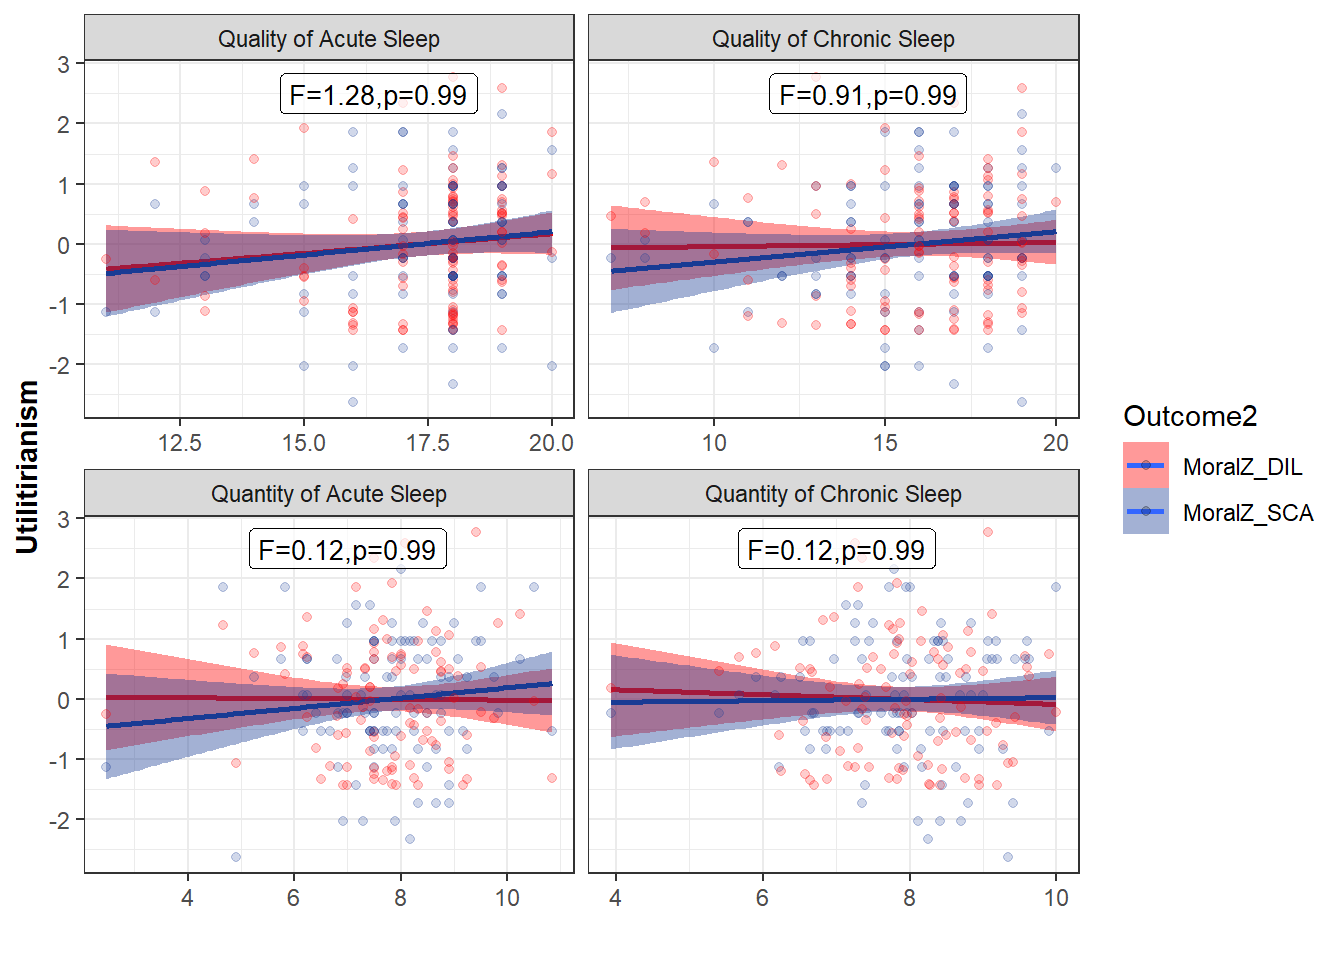
\includegraphics{SupplementaryCode_files/figure-latex/unnamed-chunk-70-1.pdf}
\textbf{N in each sleep quantity category}

\begin{Shaded}
\begin{Highlighting}[]
\NormalTok{Data_Study6_Wide}\OperatorTok{$}\NormalTok{SleepQuantCroR<-}\KeywordTok{round}\NormalTok{(Data_Study6_Wide}\OperatorTok{$}\NormalTok{SleepQuantCro)}
\NormalTok{Data_Study6_Wide}\OperatorTok{$}\NormalTok{SleepQuantAcuR<-}\KeywordTok{round}\NormalTok{(Data_Study6_Wide}\OperatorTok{$}\NormalTok{SleepQuantAcu)}

\NormalTok{Dist.Quantity.ChronicS6<-Data_Study6_Wide }\OperatorTok\StringTok{ }
\StringTok{    }\NormalTok{dplyr}\OperatorTok{::}\KeywordTok{group_by}\NormalTok{(SleepQuantCroR) }\OperatorTok\StringTok{ }
\StringTok{      }\KeywordTok{summarise}\NormalTok{(}
        \DataTypeTok{N=}\KeywordTok{n}\NormalTok{()) }\OperatorTok\StringTok{ }
\StringTok{          }\KeywordTok{spread}\NormalTok{(SleepQuantCroR, N) }\OperatorTok\StringTok{ }
\StringTok{  }\KeywordTok{as.data.frame}\NormalTok{()}
\KeywordTok{row.names}\NormalTok{(Dist.Quantity.ChronicS6)<-}\StringTok{"Quantity Chronic"}

\NormalTok{Dist.Quantity.AcuteS6<-Data_Study6_Wide }\OperatorTok\StringTok{ }
\StringTok{    }\NormalTok{dplyr}\OperatorTok{::}\KeywordTok{group_by}\NormalTok{(SleepQuantAcuR) }\OperatorTok\StringTok{ }
\StringTok{      }\KeywordTok{summarise}\NormalTok{(}
        \DataTypeTok{N=}\KeywordTok{n}\NormalTok{()) }\OperatorTok\StringTok{ }
\StringTok{          }\KeywordTok{spread}\NormalTok{(SleepQuantAcuR, N) }\OperatorTok\StringTok{ }
\StringTok{  }\KeywordTok{as.data.frame}\NormalTok{()}
\KeywordTok{row.names}\NormalTok{(Dist.Quantity.AcuteS6)<-}\StringTok{"Quantity Acute"}

\KeywordTok{bind_rows}\NormalTok{(Dist.Quantity.AcuteS6, Dist.Quantity.ChronicS6)}
\end{Highlighting}
\end{Shaded}

\begin{verbatim}
##                   2 5 6  7  8  9 10 11  4
## Quantity Acute    1 3 9 21 40 18  6  1 NA
## Quantity Chronic NA 1 6 25 40 21  5 NA  1
\end{verbatim}

\textbf{Scatterplots}

\begin{Shaded}
\begin{Highlighting}[]
\KeywordTok{ggplot}\NormalTok{(Data_ScatterS6, }\KeywordTok{aes}\NormalTok{(}\DataTypeTok{x=}\NormalTok{SleepValue, }\DataTypeTok{y=}\NormalTok{MoralValue, }\DataTypeTok{color=}\NormalTok{Outcome, }\DataTypeTok{fill=}\NormalTok{Outcome)) }\OperatorTok{+}\StringTok{ }
\StringTok{       }\KeywordTok{geom_smooth}\NormalTok{(}\DataTypeTok{method=}\StringTok{"lm"}\NormalTok{ )}\OperatorTok{+}
\StringTok{      }\KeywordTok{geom_point}\NormalTok{(}\DataTypeTok{alpha=}\FloatTok{0.2}\NormalTok{)}\OperatorTok{+}
\StringTok{       }\KeywordTok{facet_wrap}\NormalTok{(}\OperatorTok{~}\KeywordTok{factor}\NormalTok{(SleepType), }\DataTypeTok{scales=}\StringTok{"free_x"}\NormalTok{) }\OperatorTok{+}
\StringTok{       }\KeywordTok{theme_bw}\NormalTok{() }\OperatorTok{+}\StringTok{ }\KeywordTok{ylab}\NormalTok{(}\StringTok{"Utilitirianism"}\NormalTok{) }\OperatorTok{+}\StringTok{ }\KeywordTok{xlab}\NormalTok{(}\StringTok{""}\NormalTok{) }\OperatorTok{+}\StringTok{ }
\StringTok{       }\KeywordTok{theme}\NormalTok{(}\DataTypeTok{axis.title.y =} \KeywordTok{element_text}\NormalTok{(}\DataTypeTok{size =} \DecValTok{11}\NormalTok{, }\DataTypeTok{hjust =} \FloatTok{0.5}\NormalTok{, }\DataTypeTok{face=}\StringTok{"bold"}\NormalTok{), }
             \DataTypeTok{axis.title.x =} \KeywordTok{element_text}\NormalTok{(}\DataTypeTok{face=}\StringTok{"bold"}\NormalTok{, }\DataTypeTok{size =} \DecValTok{11}\NormalTok{, }\DataTypeTok{hjust =} \FloatTok{0.5}\NormalTok{)) }\OperatorTok{+}
\StringTok{       }\KeywordTok{guides}\NormalTok{(}\DataTypeTok{size=}\OtherTok{FALSE}\NormalTok{, }\DataTypeTok{colour=}\OtherTok{FALSE}\NormalTok{) }\OperatorTok{+}\StringTok{ }
\StringTok{       }\KeywordTok{scale_fill_manual}\NormalTok{(}\DataTypeTok{values=}\KeywordTok{c}\NormalTok{(}\StringTok{"red"}\NormalTok{,}\StringTok{"#193B94"}\NormalTok{))}\OperatorTok{+}
\StringTok{       }\KeywordTok{scale_color_manual}\NormalTok{(}\DataTypeTok{values=}\KeywordTok{c}\NormalTok{(}\StringTok{"red"}\NormalTok{,}\StringTok{"#193B94"}\NormalTok{))}\OperatorTok{+}

\StringTok{       }\KeywordTok{geom_label}\NormalTok{(}\DataTypeTok{data=}\NormalTok{annotationS6, }\KeywordTok{aes}\NormalTok{( }\DataTypeTok{x=}\NormalTok{x, }\DataTypeTok{y=}\NormalTok{y, }\DataTypeTok{label=}\NormalTok{label), }
                  \DataTypeTok{color=}\StringTok{"black"}\NormalTok{,  }\DataTypeTok{size=}\FloatTok{3.5}\NormalTok{ , }\DataTypeTok{angle=}\DecValTok{45}\NormalTok{, }\DataTypeTok{alpha=}\DecValTok{7}\OperatorTok{/}\DecValTok{10}\NormalTok{, }\DataTypeTok{inherit.aes =} \OtherTok{FALSE}\NormalTok{)}
\end{Highlighting}
\end{Shaded}

\includegraphics{SupplementaryCode_files/figure-latex/unnamed-chunk-72-1.pdf}

\begin{Shaded}
\begin{Highlighting}[]
\KeywordTok{library}\NormalTok{(markdown); }\KeywordTok{library}\NormalTok{(knitr); }\KeywordTok{library}\NormalTok{(gt); }\KeywordTok{library}\NormalTok{(tidyverse); }\KeywordTok{library}\NormalTok{(ggExtra); }\KeywordTok{library}\NormalTok{(effects); }\KeywordTok{library}\NormalTok{(readxl); }\KeywordTok{library}\NormalTok{(ggpubr); }\KeywordTok{library}\NormalTok{(lme4); }\KeywordTok{library}\NormalTok{(effectsize); }\KeywordTok{library}\NormalTok{(esc);}\KeywordTok{library}\NormalTok{(DescTools); }\KeywordTok{library}\NormalTok{(survey); }\KeywordTok{library}\NormalTok{(rmdformats); }\KeywordTok{library}\NormalTok{(metafor); }\KeywordTok{library}\NormalTok{(dmetar);}\KeywordTok{library}\NormalTok{(robumeta)}
\end{Highlighting}
\end{Shaded}

Combine the datasets

\begin{Shaded}
\begin{Highlighting}[]
\NormalTok{Data_MetaS1<-Data_Study1_Raw }\OperatorTok\StringTok{ }
\StringTok{  }\KeywordTok{select}\NormalTok{(ResponseId, Moral_TOT, SleepQualCro, SleepQualAcu, SleepQuantCro, SleepQuantAcu,}
\NormalTok{          Age_correct, Attention_check, CCA, Duration) }\OperatorTok\StringTok{ }
\StringTok{  }\KeywordTok{mutate}\NormalTok{(}\DataTypeTok{Outcome=}\StringTok{"Dilemmas"}\NormalTok{, }\DataTypeTok{Study=}\StringTok{"1"}\NormalTok{,}
         \DataTypeTok{ResponseId=}\KeywordTok{paste0}\NormalTok{(ResponseId, }\StringTok{"_S1"}\NormalTok{))}

\NormalTok{Data_MetaS2<-Data_Study2_Raw }\OperatorTok\StringTok{ }
\StringTok{  }\KeywordTok{select}\NormalTok{(ResponseId,Moral_TOT, SleepQualCro, SleepQualAcu, SleepQuantCro, SleepQuantAcu,}
\NormalTok{         Age_correct, Attention_check, CCA, Duration)}\OperatorTok\StringTok{ }
\StringTok{  }\KeywordTok{mutate}\NormalTok{(}\DataTypeTok{Outcome=}\StringTok{"Scale"}\NormalTok{, }\DataTypeTok{Study=}\StringTok{"2"}\NormalTok{,}
         \DataTypeTok{ResponseId=}\KeywordTok{paste0}\NormalTok{(ResponseId, }\StringTok{"_S2"}\NormalTok{))}

\NormalTok{Data_MetaS3<-Data_Study3_Raw }\OperatorTok\StringTok{ }
\StringTok{  }\KeywordTok{select}\NormalTok{(ResponseId,Moral_TOT, SleepQualCro, SleepQualAcu, SleepQuantCro, SleepQuantAcu,}
\NormalTok{         Age_correct, CCA, Duration)}\OperatorTok\StringTok{ }
\StringTok{  }\KeywordTok{mutate}\NormalTok{(}\DataTypeTok{Attention_check=}\DecValTok{1}\NormalTok{, }\DataTypeTok{Outcome=}\StringTok{"Scale"}\NormalTok{, }\DataTypeTok{Study=}\StringTok{"3"}\NormalTok{,}
         \DataTypeTok{ResponseId=}\KeywordTok{paste0}\NormalTok{(ResponseId, }\StringTok{"_S3"}\NormalTok{))}

\NormalTok{Data_MetaS4<-Data_Study4_Raw }\OperatorTok\StringTok{ }
\StringTok{  }\KeywordTok{select}\NormalTok{(ResponseId,Moral_DIL, Moral_SCA, Moral_CAR, SleepQualCro, SleepQualAcu, SleepQuantCro, SleepQuantAcu, Age_correct, Attention_check, CCA, Duration)}\OperatorTok\StringTok{ }
\StringTok{  }\KeywordTok{mutate}\NormalTok{(}\DataTypeTok{Study=}\StringTok{"4"}\NormalTok{) }\OperatorTok
\StringTok{  }\KeywordTok{pivot_longer}\NormalTok{(}\DataTypeTok{cols=}\KeywordTok{c}\NormalTok{(}\StringTok{"Moral_DIL"}\NormalTok{, }\StringTok{"Moral_SCA"}\NormalTok{, }\StringTok{"Moral_CAR"}\NormalTok{), }\DataTypeTok{names_to=}\StringTok{"Outcome_transit"}\NormalTok{) }\OperatorTok
\StringTok{  }\KeywordTok{mutate}\NormalTok{(}\DataTypeTok{Moral_TOT=}\NormalTok{value,}
         \DataTypeTok{Outcome=}\KeywordTok{case_when}\NormalTok{(}
\NormalTok{           Outcome_transit}\OperatorTok{==}\StringTok{"Moral_DIL"}\OperatorTok{~}\StringTok{"Dilemmas"}\NormalTok{,}
\NormalTok{           Outcome_transit}\OperatorTok{==}\StringTok{"Moral_SCA"}\OperatorTok{~}\StringTok{"Scale"}\NormalTok{,}
\NormalTok{           Outcome_transit}\OperatorTok{==}\StringTok{"Moral_CAR"}\OperatorTok{~}\StringTok{"Autonomouscars"}\NormalTok{),}
         \DataTypeTok{ResponseId=}\KeywordTok{paste0}\NormalTok{(ResponseId, }\StringTok{"_S4"}\NormalTok{))}

\NormalTok{Data_MetaS5<-Data_Study5_Raw }\OperatorTok\StringTok{ }
\StringTok{   }\KeywordTok{select}\NormalTok{(ResponseId,Moral_DIL, Moral_SCA, SleepQualCro, SleepQualAcu, SleepQuantCro, SleepQuantAcu,Age_correct, CCA, Duration) }\OperatorTok\StringTok{ }
\StringTok{   }\KeywordTok{pivot_longer}\NormalTok{(}\DataTypeTok{cols=}\KeywordTok{c}\NormalTok{(}\StringTok{"Moral_DIL"}\NormalTok{, }\StringTok{"Moral_SCA"}\NormalTok{), }\DataTypeTok{names_to=}\StringTok{"Outcome_transit"}\NormalTok{) }\OperatorTok
\StringTok{   }\KeywordTok{mutate}\NormalTok{(}\DataTypeTok{Moral_TOT=}\NormalTok{value, }\DataTypeTok{Attention_check=}\DecValTok{1}\NormalTok{, }\DataTypeTok{Study=}\StringTok{"5"}\NormalTok{) }\OperatorTok\StringTok{ }
\StringTok{   }\KeywordTok{mutate}\NormalTok{(}\DataTypeTok{Outcome=}\KeywordTok{case_when}\NormalTok{(}
\NormalTok{           Outcome_transit}\OperatorTok{==}\StringTok{"Moral_DIL"}\OperatorTok{~}\StringTok{"Dilemmas"}\NormalTok{,}
\NormalTok{           Outcome_transit}\OperatorTok{==}\StringTok{"Moral_SCA"}\OperatorTok{~}\StringTok{"Scale"}\NormalTok{),}
         \DataTypeTok{ResponseId=}\KeywordTok{paste0}\NormalTok{(ResponseId, }\StringTok{"_S5"}\NormalTok{))}

\NormalTok{Data_MetaS6<-Data_Study6_Raw }\OperatorTok\StringTok{ }
\StringTok{   }\KeywordTok{select}\NormalTok{(ResponseId,Moral_DIL, Moral_SCA, SleepQualCro, SleepQualAcu, SleepQuantCro, SleepQuantAcu, Age_correct, CCA,Attention_check, Duration) }\OperatorTok\StringTok{ }
\StringTok{   }\KeywordTok{pivot_longer}\NormalTok{(}\DataTypeTok{cols=}\KeywordTok{c}\NormalTok{(}\StringTok{"Moral_DIL"}\NormalTok{, }\StringTok{"Moral_SCA"}\NormalTok{), }\DataTypeTok{names_to=}\StringTok{"Outcome_transit"}\NormalTok{) }\OperatorTok
\StringTok{   }\KeywordTok{mutate}\NormalTok{(}\DataTypeTok{Moral_TOT=}\NormalTok{value, }\DataTypeTok{Study=}\StringTok{"6"}\NormalTok{) }\OperatorTok\StringTok{ }
\StringTok{   }\KeywordTok{mutate}\NormalTok{(}\DataTypeTok{Outcome=}\KeywordTok{case_when}\NormalTok{(}
\NormalTok{           Outcome_transit}\OperatorTok{==}\StringTok{"Moral_DIL"}\OperatorTok{~}\StringTok{"Dilemmas"}\NormalTok{,}
\NormalTok{           Outcome_transit}\OperatorTok{==}\StringTok{"Moral_SCA"}\OperatorTok{~}\StringTok{"Scale"}\NormalTok{),}
           \DataTypeTok{ResponseId=}\KeywordTok{paste0}\NormalTok{(ResponseId, }\StringTok{"_S6"}\NormalTok{))}

\NormalTok{Data_Meta_Raw_transit<-}\StringTok{ }\KeywordTok{bind_rows}\NormalTok{(}
\NormalTok{  Data_MetaS1, Data_MetaS2, Data_MetaS3, Data_MetaS4, Data_MetaS5, Data_MetaS6)}

\CommentTok{#Insert Participant identifier}
\NormalTok{Data_Meta_Raw <-Data_Meta_Raw_transit }\OperatorTok
\StringTok{  }\KeywordTok{mutate}\NormalTok{(}
    \DataTypeTok{Study.out.delim=}\KeywordTok{paste0}\NormalTok{(Study,}\StringTok{"_"}\NormalTok{, Outcome),}
    \DataTypeTok{VDmiss=}\KeywordTok{case_when}\NormalTok{(}
      \KeywordTok{is.na}\NormalTok{(Moral_TOT)}\OperatorTok{~}\DecValTok{1}\NormalTok{,}
      \OperatorTok{!}\KeywordTok{is.na}\NormalTok{(Moral_TOT)}\OperatorTok{~}\DecValTok{0}\NormalTok{))}
\end{Highlighting}
\end{Shaded}

Create datasets

\begin{Shaded}
\begin{Highlighting}[]
\NormalTok{Data_Meta_PRIM<-}\KeywordTok{filter}\NormalTok{(Data_Meta_Raw, Age_correct}\OperatorTok{==}\DecValTok{1} \OperatorTok{&}\StringTok{ }\NormalTok{Attention_check}\OperatorTok{==}\DecValTok{1} \OperatorTok{&}\StringTok{ }\NormalTok{CCA}\OperatorTok{==}\DecValTok{1}\NormalTok{)}
\NormalTok{Data_Meta_SENSIT1<-}\KeywordTok{filter}\NormalTok{(Data_Meta_Raw, Age_correct}\OperatorTok{==}\DecValTok{1} \OperatorTok{&}\StringTok{ }\NormalTok{Attention_check}\OperatorTok{==}\DecValTok{1} \OperatorTok{&}\StringTok{ }\NormalTok{CCA}\OperatorTok{==}\DecValTok{1} \OperatorTok{&}\StringTok{ }\NormalTok{Duration}\OperatorTok{==}\DecValTok{1}\NormalTok{)}
\NormalTok{Data_Meta_SENSIT2<-}\KeywordTok{filter}\NormalTok{(Data_Meta_Raw, Age_correct}\OperatorTok{==}\DecValTok{1} \OperatorTok{&}\StringTok{ }\NormalTok{CCA}\OperatorTok{==}\DecValTok{1}\NormalTok{)}
\NormalTok{Data_Meta_SENSIT3<-Data_Meta_Raw }\OperatorTok
\StringTok{  }\KeywordTok{group_by}\NormalTok{(ResponseId) }\OperatorTok\StringTok{ }
\StringTok{  }\KeywordTok{mutate}\NormalTok{(}\DataTypeTok{VDmissTOT =} \KeywordTok{sum}\NormalTok{(VDmiss)}\OperatorTok{/}\KeywordTok{n}\NormalTok{()) }\OperatorTok\StringTok{ }
\StringTok{  }\KeywordTok{filter}\NormalTok{(Age_correct}\OperatorTok{==}\DecValTok{1} \OperatorTok{&}\StringTok{ }\NormalTok{Attention_check}\OperatorTok{==}\DecValTok{1} \OperatorTok{&}\StringTok{ }\NormalTok{VDmissTOT}\OperatorTok{!=}\DecValTok{1}\NormalTok{)}
\NormalTok{Data_Meta_PRIM_Split<-}\KeywordTok{split}\NormalTok{(Data_Meta_PRIM, Data_Meta_PRIM}\OperatorTok{$}\NormalTok{Study.out.delim)}
\NormalTok{Data_Meta_SENSIT1_Split<-}\KeywordTok{split}\NormalTok{(Data_Meta_SENSIT1, Data_Meta_SENSIT1}\OperatorTok{$}\NormalTok{Study.out.delim)}
\NormalTok{Data_Meta_SENSIT2_Split<-}\KeywordTok{split}\NormalTok{(Data_Meta_SENSIT2, Data_Meta_SENSIT2}\OperatorTok{$}\NormalTok{Study.out.delim)}
\NormalTok{Data_Meta_SENSIT3_Split<-}\KeywordTok{split}\NormalTok{(Data_Meta_SENSIT3, Data_Meta_SENSIT3}\OperatorTok{$}\NormalTok{Study.out.delim)}
\end{Highlighting}
\end{Shaded}

Function performing correlations in each primary study and for each outcome

\begin{Shaded}
\begin{Highlighting}[]
\NormalTok{LM_perf<-}\ControlFlowTok{function}\NormalTok{(x)\{}
  \KeywordTok{list}\NormalTok{(}\KeywordTok{cor.test}\NormalTok{(}\OperatorTok{~}\NormalTok{Moral_TOT}\OperatorTok{+}\NormalTok{SleepQualCro, }\DataTypeTok{data=}\NormalTok{x,  }\DataTypeTok{conf.level =}\NormalTok{ (}\DecValTok{1}\FloatTok{-0.05}\OperatorTok{/}\DecValTok{4}\NormalTok{)),}
       \KeywordTok{cor.test}\NormalTok{(}\OperatorTok{~}\NormalTok{Moral_TOT}\OperatorTok{+}\NormalTok{SleepQualAcu, }\DataTypeTok{data=}\NormalTok{x,  }\DataTypeTok{conf.level =}\NormalTok{ (}\DecValTok{1}\FloatTok{-0.05}\OperatorTok{/}\DecValTok{4}\NormalTok{)),}
       \KeywordTok{cor.test}\NormalTok{(}\OperatorTok{~}\NormalTok{Moral_TOT}\OperatorTok{+}\NormalTok{SleepQuantCro, }\DataTypeTok{data=}\NormalTok{x,  }\DataTypeTok{conf.level =}\NormalTok{ (}\DecValTok{1}\FloatTok{-0.05}\OperatorTok{/}\DecValTok{4}\NormalTok{)),}
       \KeywordTok{cor.test}\NormalTok{(}\OperatorTok{~}\NormalTok{Moral_TOT}\OperatorTok{+}\NormalTok{SleepQuantAcu, }\DataTypeTok{data=}\NormalTok{x,  }\DataTypeTok{conf.level =}\NormalTok{ (}\DecValTok{1}\FloatTok{-0.05}\OperatorTok{/}\DecValTok{4}\NormalTok{)))}
\NormalTok{\}}
\end{Highlighting}
\end{Shaded}

Function extracting critical information from correlations

\begin{Shaded}
\begin{Highlighting}[]
\NormalTok{ExtractLM<-}\ControlFlowTok{function}\NormalTok{(x)\{}
  \KeywordTok{cbind}\NormalTok{(}
  \KeywordTok{as.numeric}\NormalTok{(x}\OperatorTok{$}\NormalTok{estimate),}
  \KeywordTok{as.numeric}\NormalTok{(x}\OperatorTok{$}\NormalTok{conf.int[}\DecValTok{1}\NormalTok{]),}
  \KeywordTok{as.numeric}\NormalTok{(x}\OperatorTok{$}\NormalTok{conf.int[}\DecValTok{2}\NormalTok{]),}
  \KeywordTok{as.numeric}\NormalTok{(x}\OperatorTok{$}\NormalTok{parameter}\OperatorTok{+}\DecValTok{2}\NormalTok{),}
  \KeywordTok{as.numeric}\NormalTok{(}\KeywordTok{escalc}\NormalTok{(}\DataTypeTok{measure=}\StringTok{"ZCOR"}\NormalTok{, }
                      \DataTypeTok{ri=}\KeywordTok{as.numeric}\NormalTok{(x}\OperatorTok{$}\NormalTok{estimate),}
                      \DataTypeTok{ni=}\KeywordTok{as.numeric}\NormalTok{(x}\OperatorTok{$}\NormalTok{parameter}\OperatorTok{+}\DecValTok{2}\NormalTok{))[}\DecValTok{1}\NormalTok{]),}
  \KeywordTok{as.numeric}\NormalTok{(}\KeywordTok{escalc}\NormalTok{(}\DataTypeTok{measure=}\StringTok{"ZCOR"}\NormalTok{, }
                      \DataTypeTok{ri=}\KeywordTok{as.numeric}\NormalTok{(x}\OperatorTok{$}\NormalTok{estimate),}
                      \DataTypeTok{ni=}\KeywordTok{as.numeric}\NormalTok{(x}\OperatorTok{$}\NormalTok{parameter}\OperatorTok{+}\DecValTok{2}\NormalTok{))[}\DecValTok{2}\NormalTok{]))}
\NormalTok{\}}
\end{Highlighting}
\end{Shaded}

Function performing meta analyses

\begin{Shaded}
\begin{Highlighting}[]
\NormalTok{Meta_perf<-}\ControlFlowTok{function}\NormalTok{(x)\{}
  \KeywordTok{robu}\NormalTok{(}
  \DataTypeTok{formula =}\NormalTok{ Fisher.Z }\OperatorTok{~}\StringTok{ }\DecValTok{1}\NormalTok{, }
  \DataTypeTok{v=}\NormalTok{Var.Fisher.Z,}
  \DataTypeTok{studynum =}\NormalTok{ Study, }
  \DataTypeTok{small =} \OtherTok{TRUE}\NormalTok{,}
  \DataTypeTok{rho=}\FloatTok{0.3}\NormalTok{,}
  \DataTypeTok{data =}\NormalTok{ x) \}}
\end{Highlighting}
\end{Shaded}

Function extracting critical information from meta analyses

\begin{Shaded}
\begin{Highlighting}[]
\NormalTok{ExtractMeta<-}\ControlFlowTok{function}\NormalTok{(x)\{}
   \KeywordTok{cbind}\NormalTok{(}
     \KeywordTok{FisherZInv}\NormalTok{(}\KeywordTok{as.numeric}\NormalTok{(x}\OperatorTok{$}\NormalTok{reg_table}\OperatorTok{$}\NormalTok{b.r)),}
     \KeywordTok{as.numeric}\NormalTok{(x}\OperatorTok{$}\NormalTok{reg_table}\OperatorTok{$}\NormalTok{prob)}\OperatorTok{*}\DecValTok{4}\NormalTok{,}
     \KeywordTok{as.numeric}\NormalTok{(x}\OperatorTok{$}\NormalTok{reg_table}\OperatorTok{$}\NormalTok{prob),}
     \KeywordTok{FisherZInv}\NormalTok{(x}\OperatorTok{$}\NormalTok{reg_table}\OperatorTok{$}\NormalTok{b.r}\OperatorTok{-}
\StringTok{               }\NormalTok{x}\OperatorTok{$}\NormalTok{reg_table}\OperatorTok{$}\NormalTok{SE}\OperatorTok{*}\NormalTok{stats}\OperatorTok{::}\KeywordTok{qt}\NormalTok{((}\DecValTok{1}\OperatorTok{-}\NormalTok{(}\FloatTok{0.05}\OperatorTok{/}\NormalTok{(}\DecValTok{2}\OperatorTok{*}\DecValTok{4}\NormalTok{))), x}\OperatorTok{$}\NormalTok{reg_table}\OperatorTok{$}\NormalTok{dfs)),}
     \KeywordTok{FisherZInv}\NormalTok{(x}\OperatorTok{$}\NormalTok{reg_table}\OperatorTok{$}\NormalTok{b.r}\OperatorTok{+}
\StringTok{               }\NormalTok{x}\OperatorTok{$}\NormalTok{reg_table}\OperatorTok{$}\NormalTok{SE}\OperatorTok{*}\NormalTok{stats}\OperatorTok{::}\KeywordTok{qt}\NormalTok{((}\DecValTok{1}\OperatorTok{-}\NormalTok{(}\FloatTok{0.05}\OperatorTok{/}\NormalTok{(}\DecValTok{2}\OperatorTok{*}\DecValTok{4}\NormalTok{))), x}\OperatorTok{$}\NormalTok{reg_table}\OperatorTok{$}\NormalTok{dfs)),}
\NormalTok{     x}\OperatorTok{$}\NormalTok{mod_info}\OperatorTok{$}\NormalTok{tau.sq,}
\NormalTok{     x}\OperatorTok{$}\NormalTok{mod_info}\OperatorTok{$}\NormalTok{I}\FloatTok{.2}\NormalTok{,}
     \KeywordTok{FisherZInv}\NormalTok{(x}\OperatorTok{$}\NormalTok{reg_table}\OperatorTok{$}\NormalTok{b.r}\OperatorTok{-}
\StringTok{               }\NormalTok{x}\OperatorTok{$}\NormalTok{reg_table}\OperatorTok{$}\NormalTok{SE}\OperatorTok{*}\NormalTok{stats}\OperatorTok{::}\KeywordTok{qt}\NormalTok{((}\DecValTok{1-2}\OperatorTok{*}\NormalTok{(}\FloatTok{0.05}\OperatorTok{/}\NormalTok{(}\DecValTok{2}\OperatorTok{*}\DecValTok{4}\NormalTok{))), x}\OperatorTok{$}\NormalTok{reg_table}\OperatorTok{$}\NormalTok{dfs)),}
     \KeywordTok{FisherZInv}\NormalTok{(x}\OperatorTok{$}\NormalTok{reg_table}\OperatorTok{$}\NormalTok{b.r}\OperatorTok{+}
\StringTok{               }\NormalTok{x}\OperatorTok{$}\NormalTok{reg_table}\OperatorTok{$}\NormalTok{SE}\OperatorTok{*}\NormalTok{stats}\OperatorTok{::}\KeywordTok{qt}\NormalTok{((}\DecValTok{1-2}\OperatorTok{*}\NormalTok{(}\FloatTok{0.05}\OperatorTok{/}\NormalTok{(}\DecValTok{2}\OperatorTok{*}\DecValTok{4}\NormalTok{))), x}\OperatorTok{$}\NormalTok{reg_table}\OperatorTok{$}\NormalTok{dfs)))}
\NormalTok{\}}
\end{Highlighting}
\end{Shaded}

\hypertarget{primary-analysis}{%
\chapter{Primary Analysis}\label{primary-analysis}}

Extracting ES for each outcome and for each primary study (Primary: 1/3)

\begin{Shaded}
\begin{Highlighting}[]
\NormalTok{List.cor.Prim<-}\KeywordTok{unlist}\NormalTok{(}\KeywordTok{lapply}\NormalTok{(Data_Meta_PRIM_Split, LM_perf), }\DataTypeTok{recursive=}\OtherTok{FALSE}\NormalTok{)}

\NormalTok{df.cor.Prim<-}\KeywordTok{data.frame}\NormalTok{(}
  \DataTypeTok{Study.out.sleep=}\KeywordTok{names}\NormalTok{(List.cor.Prim),}
  \KeywordTok{do.call}\NormalTok{(rbind,}\KeywordTok{t}\NormalTok{(}\KeywordTok{lapply}\NormalTok{(List.cor.Prim, ExtractLM))))}

\NormalTok{df.ES.Prim<-df.cor.Prim }\OperatorTok
\StringTok{  }\KeywordTok{mutate}\NormalTok{(}\DataTypeTok{Study.out.sleep=}\KeywordTok{sub}\NormalTok{(}\StringTok{"(.\{1\})$"}\NormalTok{, }\StringTok{"_}\CharTok{\textbackslash{}\textbackslash{}}\StringTok{1"}\NormalTok{, df.cor.Prim}\OperatorTok{$}\NormalTok{Study.out.sleep)) }\OperatorTok
\StringTok{  }\KeywordTok{separate}\NormalTok{(Study.out.sleep, }\DataTypeTok{into=}\KeywordTok{c}\NormalTok{(}\StringTok{"Study"}\NormalTok{, }\StringTok{"Outcome"}\NormalTok{, }\StringTok{"SleepIndicator"}\NormalTok{)) }\OperatorTok
\StringTok{  }\KeywordTok{rename}\NormalTok{(}\DataTypeTok{Raw.r=}\NormalTok{X1, }\DataTypeTok{Adj.CIlow=}\NormalTok{X2, }\DataTypeTok{Adj.CIup=}\NormalTok{X3, }\DataTypeTok{N=}\NormalTok{X4, }\DataTypeTok{Fisher.Z=}\NormalTok{X5, }\DataTypeTok{Var.Fisher.Z=}\NormalTok{X6) }\OperatorTok\StringTok{   }\KeywordTok{mutate}\NormalTok{(}
    \DataTypeTok{SleepIndicator=}\KeywordTok{case_when}\NormalTok{(}
\NormalTok{      SleepIndicator}\OperatorTok{==}\DecValTok{1}\OperatorTok{~}\StringTok{"Quality of Chronic Sleep"}\NormalTok{,}
\NormalTok{      SleepIndicator}\OperatorTok{==}\DecValTok{2}\OperatorTok{~}\StringTok{"Quality of Acute Sleep"}\NormalTok{,}
\NormalTok{      SleepIndicator}\OperatorTok{==}\DecValTok{3}\OperatorTok{~}\StringTok{"Quantity of Chronic Sleep"}\NormalTok{,}
\NormalTok{      SleepIndicator}\OperatorTok{==}\DecValTok{4}\OperatorTok{~}\StringTok{"Quantity of Acute Sleep"}\NormalTok{))}

\KeywordTok{kable}\NormalTok{(df.ES.Prim)}
\end{Highlighting}
\end{Shaded}

\begin{tabular}{l|l|l|r|r|r|r|r|r}
\hline
Study & Outcome & SleepIndicator & Raw.r & Adj.CIlow & Adj.CIup & N & Fisher.Z & Var.Fisher.Z\\
\hline
1 & Dilemmas & Quality of Chronic Sleep & 0.0211869 & -0.2048351 & 0.2450638 & 122 & 0.0211901 & 0.0084034\\
\hline
1 & Dilemmas & Quality of Acute Sleep & 0.1011547 & -0.1267766 & 0.3189396 & 122 & 0.1015018 & 0.0084034\\
\hline
1 & Dilemmas & Quantity of Chronic Sleep & -0.0003595 & -0.2253866 & 0.2247040 & 122 & -0.0003595 & 0.0084034\\
\hline
1 & Dilemmas & Quantity of Acute Sleep & 0.0741813 & -0.1534254 & 0.2943133 & 122 & 0.0743178 & 0.0084034\\
\hline
2 & Scale & Quality of Chronic Sleep & 0.0545494 & -0.1891954 & 0.2919621 & 106 & 0.0546036 & 0.0097087\\
\hline
2 & Scale & Quality of Acute Sleep & 0.0828953 & -0.1615913 & 0.3177947 & 106 & 0.0830860 & 0.0097087\\
\hline
2 & Scale & Quantity of Chronic Sleep & 0.0557577 & -0.1880266 & 0.2930704 & 106 & 0.0558156 & 0.0097087\\
\hline
2 & Scale & Quantity of Acute Sleep & 0.0363802 & -0.2066888 & 0.2752197 & 106 & 0.0363963 & 0.0097087\\
\hline
3 & Scale & Quality of Chronic Sleep & 0.1304800 & -0.2118823 & 0.4443175 & 55 & 0.1312281 & 0.0192308\\
\hline
3 & Scale & Quality of Acute Sleep & 0.0504079 & -0.2875733 & 0.3772248 & 55 & 0.0504506 & 0.0192308\\
\hline
3 & Scale & Quantity of Chronic Sleep & 0.0349274 & -0.3017354 & 0.3638455 & 55 & 0.0349417 & 0.0192308\\
\hline
3 & Scale & Quantity of Acute Sleep & -0.0383362 & -0.3668033 & 0.2986296 & 55 & -0.0383550 & 0.0192308\\
\hline
4 & Autonomouscars & Quality of Chronic Sleep & 0.0565630 & -0.1957387 & 0.3018415 & 99 & 0.0566234 & 0.0104167\\
\hline
4 & Autonomouscars & Quality of Acute Sleep & 0.0034277 & -0.2463219 & 0.2527503 & 99 & 0.0034277 & 0.0104167\\
\hline
4 & Autonomouscars & Quantity of Chronic Sleep & -0.0000723 & -0.2496067 & 0.2494710 & 99 & -0.0000723 & 0.0104167\\
\hline
4 & Autonomouscars & Quantity of Acute Sleep & -0.0384477 & -0.2852498 & 0.2131360 & 99 & -0.0384667 & 0.0104167\\
\hline
4 & Dilemmas & Quality of Chronic Sleep & -0.1858093 & -0.4160570 & 0.0668281 & 99 & -0.1879931 & 0.0104167\\
\hline
4 & Dilemmas & Quality of Acute Sleep & -0.0296262 & -0.2771164 & 0.2215505 & 99 & -0.0296349 & 0.0104167\\
\hline
4 & Dilemmas & Quantity of Chronic Sleep & -0.0038109 & -0.2531090 & 0.2459619 & 99 & -0.0038109 & 0.0104167\\
\hline
4 & Dilemmas & Quantity of Acute Sleep & 0.0674893 & -0.1851680 & 0.3117775 & 99 & 0.0675921 & 0.0104167\\
\hline
4 & Scale & Quality of Chronic Sleep & 0.0533598 & -0.1988265 & 0.2989185 & 99 & 0.0534105 & 0.0104167\\
\hline
4 & Scale & Quality of Acute Sleep & -0.0401589 & -0.2868235 & 0.2114994 & 99 & -0.0401806 & 0.0104167\\
\hline
4 & Scale & Quantity of Chronic Sleep & -0.1030109 & -0.3437145 & 0.1503939 & 99 & -0.1033776 & 0.0104167\\
\hline
4 & Scale & Quantity of Acute Sleep & -0.0281352 & -0.2757382 & 0.2229691 & 99 & -0.0281426 & 0.0104167\\
\hline
5 & Dilemmas & Quality of Chronic Sleep & -0.0775263 & -0.3140136 & 0.1680191 & 105 & -0.0776822 & 0.0098039\\
\hline
5 & Dilemmas & Quality of Acute Sleep & 0.0697277 & -0.1756287 & 0.3069283 & 105 & 0.0698410 & 0.0098039\\
\hline
5 & Dilemmas & Quantity of Chronic Sleep & -0.0660172 & -0.3035479 & 0.1792391 & 105 & -0.0661133 & 0.0098039\\
\hline
5 & Dilemmas & Quantity of Acute Sleep & 0.0496814 & -0.1950556 & 0.2885942 & 105 & 0.0497223 & 0.0098039\\
\hline
5 & Scale & Quality of Chronic Sleep & 0.0590484 & -0.1860018 & 0.2971830 & 105 & 0.0591172 & 0.0098039\\
\hline
5 & Scale & Quality of Acute Sleep & 0.0520815 & -0.1927397 & 0.2907986 & 105 & 0.0521287 & 0.0098039\\
\hline
5 & Scale & Quantity of Chronic Sleep & -0.0205720 & -0.2616553 & 0.2229277 & 105 & -0.0205749 & 0.0098039\\
\hline
5 & Scale & Quantity of Acute Sleep & -0.0245128 & -0.2653244 & 0.2191776 & 105 & -0.0245177 & 0.0098039\\
\hline
6 & Dilemmas & Quality of Chronic Sleep & 0.0181003 & -0.2324887 & 0.2664357 & 99 & 0.0181023 & 0.0104167\\
\hline
6 & Dilemmas & Quality of Acute Sleep & 0.1068219 & -0.1466255 & 0.3471082 & 99 & 0.1072310 & 0.0104167\\
\hline
6 & Dilemmas & Quantity of Chronic Sleep & -0.0422104 & -0.2887083 & 0.2095355 & 99 & -0.0422355 & 0.0104167\\
\hline
6 & Dilemmas & Quantity of Acute Sleep & -0.0082190 & -0.2572303 & 0.2418158 & 99 & -0.0082192 & 0.0104167\\
\hline
6 & Scale & Quality of Chronic Sleep & 0.1340424 & -0.1194934 & 0.3711662 & 99 & 0.1348540 & 0.0104167\\
\hline
6 & Scale & Quality of Acute Sleep & 0.1399702 & -0.1135342 & 0.3763635 & 99 & 0.1408952 & 0.0104167\\
\hline
6 & Scale & Quantity of Chronic Sleep & 0.0132858 & -0.2370389 & 0.2619562 & 99 & 0.0132866 & 0.0104167\\
\hline
6 & Scale & Quantity of Acute Sleep & 0.1059963 & -0.1474424 & 0.3463736 & 99 & 0.1063960 & 0.0104167\\
\hline
\end{tabular}

robu(
formula = Fisher.Z \textasciitilde{} 1,
v=Var.Fisher.Z,
studynum = Study,
small = TRUE,
rho=0.3,
data = x)

summary(lmer(Moral\_TOT\textasciitilde SleepQualAcu+(1+SleepQualAcu\textbar Study/Outcome), data=Data\_Meta\_PRIM))
summary(lmer(Moral\_TOT\textasciitilde SleepQuantCro+(1\textbar Study/Outcome) + (SleepQuantCro-1\textbar Study/Outcome), data=Data\_Meta\_PRIM))

Z\textless- rma.mv(Fisher.Z, Var.Fisher.Z, random = \textasciitilde{} 1 \textbar Study/Outcome, data=Data\_Meta\_ES\_prim{[}Data\_Meta\_ES\_prim\$SleepIndicator==``Quality of Acute Sleep'',{]})

robust(Z, cluster = subset(Data\_Meta\_ES\_prim\(Study, Data_Meta_ES_prim\)SleepIndicator==``Quality of Acute Sleep''))

library(clubSandwich)

conf\_int(res, vcov = ``CR2'')

Perform Primary Meta Analysis (Primary: 2/3)

\begin{Shaded}
\begin{Highlighting}[]
\NormalTok{df.ES.Prim.Split<-}\KeywordTok{split}\NormalTok{(df.ES.Prim, df.ES.Prim}\OperatorTok{$}\NormalTok{SleepIndicator)}

\NormalTok{df.Meta.Res1.Prim<-}\KeywordTok{lapply}\NormalTok{(df.ES.Prim.Split, Meta_perf)}

\NormalTok{df.Meta.Res2.Prim<-}\KeywordTok{as.data.frame}\NormalTok{(}\KeywordTok{t}\NormalTok{(}\KeywordTok{sapply}\NormalTok{(df.Meta.Res1.Prim, ExtractMeta)))}

\NormalTok{df.Meta.Res3.Prim<-}\KeywordTok{as.data.frame}\NormalTok{(}\KeywordTok{cbind}\NormalTok{(}\DataTypeTok{SleepIndicator=}\KeywordTok{row.names}\NormalTok{(df.Meta.Res2.Prim),}
\NormalTok{                                         df.Meta.Res2.Prim))}
\NormalTok{df.Meta.Prim<-}\StringTok{ }\NormalTok{df.Meta.Res3.Prim }\OperatorTok\StringTok{ }
\StringTok{  }\KeywordTok{rename}\NormalTok{(}\DataTypeTok{Raw.r=}\NormalTok{V1, }\DataTypeTok{Adj.pval=}\NormalTok{V2, }\DataTypeTok{Raw.pval=}\NormalTok{V3, }\DataTypeTok{Adj.CIlow=}\NormalTok{V4, }\DataTypeTok{Adj.CIup=}\NormalTok{V5,}
         \DataTypeTok{Tau=}\NormalTok{V6, }\DataTypeTok{I.squared=}\NormalTok{V7, }\DataTypeTok{TOST1=}\NormalTok{V8, }\DataTypeTok{TOST2=}\NormalTok{V9) }\OperatorTok
\StringTok{  }\KeywordTok{rowwise}\NormalTok{() }\OperatorTok
\StringTok{  }\KeywordTok{mutate}\NormalTok{(}\DataTypeTok{Study=}\StringTok{"Pooled Effect Size"}\NormalTok{,}
         \DataTypeTok{Outcome=}\StringTok{"All outcomes"}\NormalTok{,}
         \DataTypeTok{Adj.pval=}\KeywordTok{case_when}\NormalTok{(}
\NormalTok{           Adj.pval}\OperatorTok{>}\NormalTok{.}\DecValTok{99}\OperatorTok{~}\NormalTok{.}\DecValTok{99}\NormalTok{,}
\NormalTok{           Adj.pval}\OperatorTok{<=}\NormalTok{.}\DecValTok{99}\OperatorTok{~}\NormalTok{Adj.pval),}
         \DataTypeTok{TOST=}\KeywordTok{max}\NormalTok{(}\KeywordTok{abs}\NormalTok{(TOST1), }\KeywordTok{abs}\NormalTok{(TOST2)))}

\NormalTok{df.Meta.Prim}
\end{Highlighting}
\end{Shaded}

\begin{verbatim}
## # A tibble: 4 x 13
## # Rowwise: 
##   SleepIndicator    Raw.r Adj.pval Raw.pval Adj.CIlow Adj.CIup   Tau I.squared
##   <fct>             <dbl>    <dbl>    <dbl>     <dbl>    <dbl> <dbl>     <dbl>
## 1 Quality of Ac~  0.0690     0.102   0.0255   -0.0150   0.152      0         0
## 2 Quality of Ch~  0.0332     0.594   0.148    -0.0422   0.108      0         0
## 3 Quantity of A~  0.0293     0.410   0.103    -0.0275   0.0858     0         0
## 4 Quantity of C~ -0.00303    0.99    0.858    -0.0658   0.0598     0         0
## # ... with 5 more variables: TOST1 <dbl>, TOST2 <dbl>, Study <chr>,
## #   Outcome <chr>, TOST <dbl>
\end{verbatim}

Dataset with summary results (Primary: 3/3)

\begin{Shaded}
\begin{Highlighting}[]
\NormalTok{df.Summary.Prim.transit <-}\StringTok{ }\KeywordTok{bind_rows}\NormalTok{(df.Meta.Prim, df.ES.Prim)}
  
\NormalTok{df.Summary.Prim<-}\StringTok{ }\NormalTok{df.Summary.Prim.transit }\OperatorTok\StringTok{ }
\StringTok{  }\KeywordTok{select}\NormalTok{(SleepIndicator, Study, Outcome, Raw.r,Raw.pval, Adj.pval, Adj.CIlow, Adj.CIup, N, Tau, I.squared, TOST) }\OperatorTok
\StringTok{  }\KeywordTok{group_by}\NormalTok{(SleepIndicator) }\OperatorTok\StringTok{ }
\StringTok{  }\KeywordTok{mutate}\NormalTok{(}\DataTypeTok{Nobs=}\KeywordTok{sum}\NormalTok{(N,}\DataTypeTok{na.rm=}\NormalTok{T)) }
         
\NormalTok{df.Summary.Prim}\OperatorTok{$}\NormalTok{SleepIndicator <-}\StringTok{ }\KeywordTok{factor}\NormalTok{(df.Summary.Prim}\OperatorTok{$}\NormalTok{SleepIndicator)  }
\NormalTok{df.Summary.Prim}\OperatorTok{$}\NormalTok{SleepIndicator <-}\StringTok{ }\KeywordTok{factor}\NormalTok{(df.Summary.Prim}\OperatorTok{$}\NormalTok{SleepIndicator,}
  \DataTypeTok{levels=}\KeywordTok{rev}\NormalTok{(}\KeywordTok{levels}\NormalTok{(df.Summary.Prim}\OperatorTok{$}\NormalTok{SleepIndicator)))}

\NormalTok{df.Summary.Prim}\OperatorTok{$}\NormalTok{Study <-}\StringTok{ }\KeywordTok{factor}\NormalTok{(df.Summary.Prim}\OperatorTok{$}\NormalTok{Study)  }
\NormalTok{df.Summary.Prim}\OperatorTok{$}\NormalTok{Study <-}\StringTok{ }\KeywordTok{factor}\NormalTok{(df.Summary.Prim}\OperatorTok{$}\NormalTok{Study, }
  \DataTypeTok{levels=}\KeywordTok{rev}\NormalTok{(}\KeywordTok{levels}\NormalTok{(df.Summary.Prim}\OperatorTok{$}\NormalTok{Study)))}

\NormalTok{df.Summary.Prim}\OperatorTok{$}\NormalTok{Outcome<-}\StringTok{ }\KeywordTok{factor}\NormalTok{(df.Summary.Prim}\OperatorTok{$}\NormalTok{Outcome)  }
\KeywordTok{levels}\NormalTok{(df.Summary.Prim}\OperatorTok{$}\NormalTok{Outcome)}
\end{Highlighting}
\end{Shaded}

\begin{verbatim}
## [1] "All outcomes"   "Autonomouscars" "Dilemmas"       "Scale"
\end{verbatim}

\begin{Shaded}
\begin{Highlighting}[]
\KeywordTok{levels}\NormalTok{(df.Summary.Prim}\OperatorTok{$}\NormalTok{Study)}
\end{Highlighting}
\end{Shaded}

\begin{verbatim}
## [1] "Pooled Effect Size" "6"                  "5"                 
## [4] "4"                  "3"                  "2"                 
## [7] "1"
\end{verbatim}

\begin{Shaded}
\begin{Highlighting}[]
\NormalTok{df.Summary.Prim}
\end{Highlighting}
\end{Shaded}

\begin{verbatim}
## # A tibble: 44 x 13
## # Groups:   SleepIndicator [4]
##    SleepIndicator Study Outcome    Raw.r Raw.pval Adj.pval Adj.CIlow Adj.CIup
##    <fct>          <fct> <fct>      <dbl>    <dbl>    <dbl>     <dbl>    <dbl>
##  1 Quality of Ac~ Pool~ All ou~  6.90e-2   0.0255    0.102   -0.0150   0.152 
##  2 Quality of Ch~ Pool~ All ou~  3.32e-2   0.148     0.594   -0.0422   0.108 
##  3 Quantity of A~ Pool~ All ou~  2.93e-2   0.103     0.410   -0.0275   0.0858
##  4 Quantity of C~ Pool~ All ou~ -3.03e-3   0.858     0.99    -0.0658   0.0598
##  5 Quality of Ch~ 1     Dilemm~  2.12e-2  NA        NA       -0.205    0.245 
##  6 Quality of Ac~ 1     Dilemm~  1.01e-1  NA        NA       -0.127    0.319 
##  7 Quantity of C~ 1     Dilemm~ -3.59e-4  NA        NA       -0.225    0.225 
##  8 Quantity of A~ 1     Dilemm~  7.42e-2  NA        NA       -0.153    0.294 
##  9 Quality of Ch~ 2     Scale    5.45e-2  NA        NA       -0.189    0.292 
## 10 Quality of Ac~ 2     Scale    8.29e-2  NA        NA       -0.162    0.318 
## # ... with 34 more rows, and 5 more variables: N <dbl>, Tau <dbl>,
## #   I.squared <dbl>, TOST <dbl>, Nobs <dbl>
\end{verbatim}

Plot primary Analysis

\begin{Shaded}
\begin{Highlighting}[]
\NormalTok{p<-}\KeywordTok{ggplot}\NormalTok{(}\DataTypeTok{data=}\NormalTok{df.Summary.Prim)}\OperatorTok{+}
\StringTok{  }\KeywordTok{geom_point}\NormalTok{(}\KeywordTok{aes}\NormalTok{(}\DataTypeTok{x =}\NormalTok{ Study, }\DataTypeTok{y =}\NormalTok{ Raw.r, }\DataTypeTok{shape=}\NormalTok{Outcome, }
                 \DataTypeTok{colour=}\NormalTok{Study, }\DataTypeTok{fill=}\NormalTok{Study, }\DataTypeTok{size=}\KeywordTok{ordered}\NormalTok{(Study)),}
             \DataTypeTok{position=}\KeywordTok{position_dodge2}\NormalTok{(}\DataTypeTok{width=}\DecValTok{8}\NormalTok{))}\OperatorTok{+}\StringTok{ }
\StringTok{  }
\StringTok{  }\KeywordTok{geom_pointrange}\NormalTok{(}\DataTypeTok{position=}\KeywordTok{position_dodge2}\NormalTok{(}\DataTypeTok{width=}\DecValTok{8}\NormalTok{), }
                  \KeywordTok{aes}\NormalTok{(}\DataTypeTok{x =}\NormalTok{ Study, }\DataTypeTok{y =}\NormalTok{ Raw.r, }
                      \DataTypeTok{ymin =}\NormalTok{ Adj.CIlow, }\DataTypeTok{ymax =}\NormalTok{ Adj.CIup,  }\DataTypeTok{shape=}\NormalTok{Outcome,}
                      \DataTypeTok{linetype=}\NormalTok{Study, }\DataTypeTok{colour=}\NormalTok{Study, }\DataTypeTok{fill=}\NormalTok{Study))}\OperatorTok{+}

\StringTok{  }\KeywordTok{geom_hline}\NormalTok{(}\DataTypeTok{yintercept =}\DecValTok{0}\NormalTok{, }\DataTypeTok{linetype=}\DecValTok{2}\NormalTok{)}\OperatorTok{+}
\StringTok{  }\KeywordTok{xlab}\NormalTok{(}\StringTok{''}\NormalTok{)}\OperatorTok{+}\StringTok{ }\KeywordTok{ylab}\NormalTok{(}\StringTok{"Correlation coefficient (95% Confidence Interval)"}\NormalTok{)}\OperatorTok{+}
\StringTok{  }\KeywordTok{facet_wrap}\NormalTok{(}\OperatorTok{~}\NormalTok{SleepIndicator,}
               \DataTypeTok{strip.position=}\StringTok{"top"}\NormalTok{,}
               \DataTypeTok{ncol=}\DecValTok{2}\NormalTok{, }\DataTypeTok{nrow=}\DecValTok{2}\NormalTok{,}\DataTypeTok{scales =} \StringTok{"free_y"}\NormalTok{) }\OperatorTok{+}
\StringTok{  }\KeywordTok{coord_flip}\NormalTok{()}\OperatorTok{+}
\StringTok{  }\KeywordTok{theme_bw}\NormalTok{() }\OperatorTok{+}
\StringTok{  }\KeywordTok{theme}\NormalTok{(}\DataTypeTok{legend.position=}\StringTok{"right"}\NormalTok{,}
        \CommentTok{# plot.margin = unit(c(0.1, 0.1, 0.1, 0.1), "cm"),}
          \DataTypeTok{axis.text.y=}\KeywordTok{element_blank}\NormalTok{(),}
          \DataTypeTok{axis.ticks.y=}\KeywordTok{element_blank}\NormalTok{(),}
          \DataTypeTok{axis.text.x=}\KeywordTok{element_text}\NormalTok{(}\DataTypeTok{size=}\DecValTok{10}\NormalTok{, }\DataTypeTok{face=}\StringTok{"bold"}\NormalTok{),}
          \DataTypeTok{axis.title.y=}\KeywordTok{element_text}\NormalTok{(}\DataTypeTok{size=}\DecValTok{12}\NormalTok{,}\DataTypeTok{face=}\StringTok{"bold"}\NormalTok{),}
          \DataTypeTok{axis.title.x=}\KeywordTok{element_text}\NormalTok{(}\DataTypeTok{size=}\DecValTok{12}\NormalTok{,}\DataTypeTok{face=}\StringTok{"bold"}\NormalTok{),}
          \DataTypeTok{strip.text.x =} \KeywordTok{element_text}\NormalTok{(}\DataTypeTok{hjust=}\FloatTok{0.5}\NormalTok{,}\DataTypeTok{vjust =}\FloatTok{0.5}\NormalTok{,}\DataTypeTok{angle=}\DecValTok{0}\NormalTok{,}
                                      \DataTypeTok{size=}\DecValTok{11}\NormalTok{),}
          \DataTypeTok{legend.background =} \KeywordTok{element_rect}\NormalTok{(}\DataTypeTok{size=}\FloatTok{0.5}\NormalTok{, }\DataTypeTok{linetype=}\StringTok{"solid"}\NormalTok{, }
                                  \DataTypeTok{colour =}\StringTok{"black"}\NormalTok{),}
        \DataTypeTok{legend.box =} \StringTok{"vertical"}\NormalTok{)}\OperatorTok{+}
\StringTok{        }\CommentTok{#legend.title = element_text(size=10, face="bold"),}
\StringTok{        }\CommentTok{# legend.position = "none")+}
\StringTok{        }\CommentTok{#panel.spacing.x = unit(2.5, "cm"),}
\StringTok{  }\KeywordTok{scale_linetype_manual}\NormalTok{(}\DataTypeTok{values=}\KeywordTok{c}\NormalTok{(}\StringTok{"solid"}\NormalTok{, }\KeywordTok{rep}\NormalTok{(}\StringTok{"solid"}\NormalTok{,}\DataTypeTok{each=}\DecValTok{10}\NormalTok{)))}\OperatorTok{+}\CommentTok{#longdash}
\StringTok{  }\KeywordTok{scale_shape_manual}\NormalTok{(}\DataTypeTok{name=}\StringTok{""}\NormalTok{, }
                     \DataTypeTok{values=}\KeywordTok{c}\NormalTok{(}\DecValTok{22}\NormalTok{, }\DecValTok{23}\NormalTok{, }\DecValTok{16}\NormalTok{,}\DecValTok{17}\NormalTok{),}
                     \DataTypeTok{guide=}\KeywordTok{guide_legend}\NormalTok{(}\DataTypeTok{reverse=}\NormalTok{T))  }\OperatorTok{+}\StringTok{ }
\StringTok{  }\KeywordTok{scale_color_manual}\NormalTok{(}\DataTypeTok{values =} \KeywordTok{c}\NormalTok{(}\StringTok{"red"}\NormalTok{, }
                                    \StringTok{"#CC00E8"}\NormalTok{,}
                                    \StringTok{"#7B00CB"}\NormalTok{,}
                                    \StringTok{"#1C0082"}\NormalTok{,}
                                    \StringTok{"#016EB0"}\NormalTok{, }
                                    \StringTok{"#0390FE"}\NormalTok{,}
                                    \StringTok{"#60C3FF"}\NormalTok{), }
                       \DataTypeTok{name=}\StringTok{""}\NormalTok{,}
                       \DataTypeTok{labels=}\KeywordTok{c}\NormalTok{(}\StringTok{"Pooled"}\NormalTok{,  }
                                \StringTok{"Study 6"}\NormalTok{,}
                                \StringTok{"Study 5"}\NormalTok{,}
                                \StringTok{"Study 4"}\NormalTok{, }
                                \StringTok{"Study 3"}\NormalTok{,}
                                \StringTok{"Study 2"}\NormalTok{,}
                                \StringTok{"Study 1"}\NormalTok{),}
                       \DataTypeTok{guide=}\KeywordTok{guide_legend}\NormalTok{(}\DataTypeTok{reverse=}\NormalTok{T))   }\OperatorTok{+}
\StringTok{      }\KeywordTok{scale_fill_manual}\NormalTok{(}\DataTypeTok{values =} \KeywordTok{c}\NormalTok{(}\StringTok{"red"}\NormalTok{, }
                                   \StringTok{"#CC00E8"}\NormalTok{,}
                                   \StringTok{"#7B00CB"}\NormalTok{,}
                                   \StringTok{"#1C0082"}\NormalTok{, }
                                   \StringTok{"#016EB0"}\NormalTok{, }
                                   \StringTok{"#0390FE"}\NormalTok{,}
                                   \StringTok{"#60C3FF"}\NormalTok{), }
                       \DataTypeTok{name=}\StringTok{""}\NormalTok{,}
                       \DataTypeTok{guide=}\KeywordTok{guide_legend}\NormalTok{(}\DataTypeTok{reverse=}\NormalTok{T)) }\OperatorTok{+}\StringTok{ }\CommentTok{#+}
\KeywordTok{scale_size_manual}\NormalTok{(}\DataTypeTok{values=}\KeywordTok{c}\NormalTok{(}\DecValTok{6}\NormalTok{, }\KeywordTok{rep}\NormalTok{(}\DecValTok{4}\NormalTok{, }\DecValTok{6}\NormalTok{))) }

\NormalTok{p}\OperatorTok{+}\KeywordTok{guides}\NormalTok{( }\DataTypeTok{shape=}\OtherTok{FALSE}\NormalTok{,}\DataTypeTok{fill =} \OtherTok{FALSE}\NormalTok{,  }\DataTypeTok{size=}\OtherTok{FALSE}\NormalTok{,}\DataTypeTok{linetype=}\OtherTok{FALSE}\NormalTok{)}\CommentTok{#}
\end{Highlighting}
\end{Shaded}

\includegraphics{SupplementaryCode_files/figure-latex/unnamed-chunk-83-1.pdf}

  \bibliography{book.bib,packages.bib}

\end{document}
